\PassOptionsToPackage{unicode=true}{hyperref} % options for packages loaded elsewhere
\PassOptionsToPackage{hyphens}{url}
%
\documentclass[]{book}
\usepackage{lmodern}
\usepackage{amssymb,amsmath}
\usepackage{ifxetex,ifluatex}
\usepackage{fixltx2e} % provides \textsubscript
\ifnum 0\ifxetex 1\fi\ifluatex 1\fi=0 % if pdftex
  \usepackage[T1]{fontenc}
  \usepackage[utf8]{inputenc}
  \usepackage{textcomp} % provides euro and other symbols
\else % if luatex or xelatex
  \usepackage{unicode-math}
  \defaultfontfeatures{Ligatures=TeX,Scale=MatchLowercase}
\fi
% use upquote if available, for straight quotes in verbatim environments
\IfFileExists{upquote.sty}{\usepackage{upquote}}{}
% use microtype if available
\IfFileExists{microtype.sty}{%
\usepackage[]{microtype}
\UseMicrotypeSet[protrusion]{basicmath} % disable protrusion for tt fonts
}{}
\IfFileExists{parskip.sty}{%
\usepackage{parskip}
}{% else
\setlength{\parindent}{0pt}
\setlength{\parskip}{6pt plus 2pt minus 1pt}
}
\usepackage{hyperref}
\hypersetup{
            pdftitle={Mind, Brain, Body},
            pdfauthor={By: Bridget Callaghan, Emily Towner, Kristen Chu},
            pdfborder={0 0 0},
            breaklinks=true}
\urlstyle{same}  % don't use monospace font for urls
\usepackage{longtable,booktabs}
% Fix footnotes in tables (requires footnote package)
\IfFileExists{footnote.sty}{\usepackage{footnote}\makesavenoteenv{longtable}}{}
\usepackage{graphicx,grffile}
\makeatletter
\def\maxwidth{\ifdim\Gin@nat@width>\linewidth\linewidth\else\Gin@nat@width\fi}
\def\maxheight{\ifdim\Gin@nat@height>\textheight\textheight\else\Gin@nat@height\fi}
\makeatother
% Scale images if necessary, so that they will not overflow the page
% margins by default, and it is still possible to overwrite the defaults
% using explicit options in \includegraphics[width, height, ...]{}
\setkeys{Gin}{width=\maxwidth,height=\maxheight,keepaspectratio}
\setlength{\emergencystretch}{3em}  % prevent overfull lines
\providecommand{\tightlist}{%
  \setlength{\itemsep}{0pt}\setlength{\parskip}{0pt}}
\setcounter{secnumdepth}{5}
% Redefines (sub)paragraphs to behave more like sections
\ifx\paragraph\undefined\else
\let\oldparagraph\paragraph
\renewcommand{\paragraph}[1]{\oldparagraph{#1}\mbox{}}
\fi
\ifx\subparagraph\undefined\else
\let\oldsubparagraph\subparagraph
\renewcommand{\subparagraph}[1]{\oldsubparagraph{#1}\mbox{}}
\fi

% set default figure placement to htbp
\makeatletter
\def\fps@figure{htbp}
\makeatother

\usepackage{booktabs}
\usepackage{amsthm}
\makeatletter
\def\thm@space@setup{%
  \thm@preskip=8pt plus 2pt minus 4pt
  \thm@postskip=\thm@preskip
}
\makeatother
\usepackage[]{natbib}
\bibliographystyle{apalike}

\title{Mind, Brain, Body}
\author{By: Bridget Callaghan, Emily Towner, Kristen Chu}
\date{Updated on: 2020-08-24}

\begin{document}
\maketitle

{
\setcounter{tocdepth}{1}
\tableofcontents
}
\hypertarget{section}{%
\chapter{}\label{section}}

\begin{figure}
\centering

\includegraphics{images/index/banner.png}
\caption{}
\end{figure}

The Mind, Brain, Body study looks at how early caregiving experiences influence emotional, cognitive, and brain development, as well as physical health and wellness.

The study also explores how the bacteria that live inside us (the microbiome) are connected to the development of our brains and bodies.

\hypertarget{information}{%
\chapter{Information}\label{information}}

\hypertarget{summary}{%
\section{Summary}\label{summary}}

\hypertarget{abstract}{%
\subsection{Abstract}\label{abstract}}

The Mind, Brain, Body (MBB) study examines links between early life adversity (ELA), the gastrointestinal microbiome, memory and affective neurodevelopment, across three years in middle childhood through adolescence. The specific aims of this study are to (1) determine how adversity affects developmental change in the microbiome in middle childhood and adolescence, (2) establish associations between the microbiome, memory development, and the hippocampus, and (3) identify independent and joint influences of adversity exposure, the microbiome, brain and memory performance on the emergence of anxiety symptoms across development. We are recruiting N = 75 ELA exposed, and N = 75 not adversity exposed (Comparison) children and adolescents to take part in 3 waves of data collection. Children in the ELA group must be 6-16 years of age, while children in the comparison group must be 6-9 or 13-16 years of age. Participants complete a laboratory session (in-person or online) in Wave 1-3, and also complete a neuroimaging session in Wave 2. Study procedures for the laboratory session in Wave 1-3 remain similar. For the ELA group, we are recruiting youth who were adopted from institutional or foster care: previously institutionalized and who are now adopted internationally (PI), adopted domestically from foster care (DA). Comparison youth have not experienced these forms of early life caregiving adversities (i.e., they have always been with their biological parents). In addition to the primary aims of the MBB study, described above, we are also collecting a range of supplemental biological, questionnaire, and MRI measures aimed at assessing cognitive and emotional functioning, family functioning, as well as immune, biomarkers, and physical health assessments to aid in understanding the mechanisms behind the specific aims under investigation. The MBB study will test for links between the microbiome, memory, hippocampal function, and anxiety across a three-year time frame in middle childhood -- adolescence (6-16 years of age). Participants may opt out of the study at any point in time but will be asked to participate in testing every year until funding ceases (current grant funding this research -- R00 NIMH -- ends in 2022).

\begin{center}\rule{0.5\linewidth}{0.5pt}\end{center}

\hypertarget{aims}{%
\subsection{Aims}\label{aims}}

The study will test four primary and two supplemental hypotheses. The primary hypotheses are: (H1) that there will be greater stability in microbiome composition across 3 years in the ELA than Comparison group, (H2) ELA will be associated with higher expression of anxiety symptoms across time, (H3) the microbiome in Wave 1 will predict developmental change in memory performance between Wave 1-3, and that hippocampal activity during learning will mediate that association, (H4) that the microbiome, hippocampal encoding patterns, and memory behavior longitudinally mediate the adversity and anxiety association across development. The supplemental hypotheses are: (SH1) that ELA will be associated with a higher incidence of physical health (particularly gastrointestinal) problems, as well as dysregulation in stress response and immune systems, (SH2) that physical symptoms, stress response and immune system will mediate the link between adversity exposure, microbiome changes, hippocampal neurodevelopment, and memory.

\begin{center}\rule{0.5\linewidth}{0.5pt}\end{center}

\hypertarget{background}{%
\subsection{Background}\label{background}}

An individuals early rearing history has a significant effect on their emotional functioning across the lifespan. In particular, access to consistent/stable caregivers is strongly associated with mental health \citep{repetti_2002}, and parent-related early adversities (e.g., abuse and neglect) contribute to more than a third of mental illnesses \citep[anxiety being the most common diagnosis;][]{kessler_2005}. Clinical, epidemiological and basic science suggests that two systems affected by early adversity -- the gastrointestinal microbiome, and the hippocampal memory system, are also consistently associated with the emergence and maintenance of anxiety symptoms. Rodent and monkey models have established that adversity alters microbial communities in the gut \citep{bailey_1999, bailey_2010, omahony_2009} and that microbial populations are causally related to the expression of anxious behaviors \citep{collins_2013}. In humans too, microbiome-related gastrointestinal disturbances (e.g., irritable bowel syndrome) and anxiety are highly comorbid \citep{kennedy_2014, callaghan_2019}. In terms of the memory system, rodent studies show that typically weak memories in childhood get stronger following adversity \citetext{\citealp{callaghan_2012a}; \citealp[callaghan\_2012b;][]{cowan_2013}}, and exposure to early stress promotes hippocampal synaptic development \citep{huang_2005}, which aids long-term memory persistence. Memory dysfunction is key to maintaining anxiety disorders, which are characterized by persistent and intrusive memories of threat\citep{acheson_2012, zlomuzica_2014}, and hippocampal dysfunction is common in anxiety disorders \citep{godsil_2013}. Importantly, hippocampal development is causally tied to the microbiome in early life \citep{callaghan_2016, clarke_2013, cowan_2016, gareau_2011}, suggesting that interactions between these two systems could contribute to anxiety emergence. Although microbial and hippocampal memory systems exert their effects on anxiety in the context of one another, until now, they have always been studied independently.

Using a completely novel longitudinal design, we will test the hypothesis that changes in the gastrointestinal microbiome are associated with early adverse caregiving and underlie altered hippocampal development and memory functioning in middle childhood -- adolescence. Moreover, we will examine whether those microbial, and neurodevelopmental changes mediate the progression towards anxiety symptoms in early adversity exposed individuals. To answer these questions, we will compare longitudinal data from a group of adolescents who have experienced early caregiving adversity, to a group of comparison youth who have not experienced those same events. The study will involve examining the gastrointestinal microbiome (measured through stool samples), and functional magnetic resonance imaging (fMRI) to understand hippocampal functional development. In addition, the study will collect saliva and blood spot samples to assess saliva biomarkers (e.g., cortisol, testosterone) and blood immune markers (e.g., CRP, interleukins), as well as hair samples to assess chronic cortisol exposure, which can be used to understand the mechanisms behind microbiome-brain associations in youth.

\begin{center}\rule{0.5\linewidth}{0.5pt}\end{center}

\hypertarget{procedure}{%
\section{Procedure}\label{procedure}}

All youth will be recruited through community settings, clinics (e.g., pediatricians office), specialized services (e.g., adoption services), and through the internet (community boards, targeted advertisements).

Three assessments (spaced 12 months apart -- Wave 1-3) will occur with youth who fall within the period of development in the hippocampal and microbiome: `children', and `adolescents' aged 6-16 years. Biological (stool, saliva, blood spots, hair), questionnaire, and behavioral data will be collected in each wave of the study, and an fMRI scan will be collected in Wave 2. Participants will be recruited who have either experienced early life adversity (ELA) through adverse caregiving (previously institutionalized, domestically adopted), or who have not been exposed to those caregiving experiences (Comparison). A sample size of N = 75 youth will be recruited into each of those groups, resulting in a final target of N = 150 youth in the study (N = 37-38 in each of the age groups = children versus adolescents, for the ELA and Comparison groups at Wave 1). That target sample size takes attrition into account across the longitudinal study (expected at 20\%, to arrive at a final sample size of N = 120). Study procedures for each wave of data collection will be similar, except for Wave 2 where an fMRI scan will occur in a second session. In addition, Wave 1 of data collection was transitioned online due to the outbreak of the global COVID-19 pandemic.

Participants will therefore range in age from 6-16 years at Wave 1, 7-17 years at Wave 2, and 8-20 years at Wave 3. Participants will be recruited through targeted mailout (birth records), online advertising (e.g., Craigslist), school and community organization partnerships, street-fairs and community gathering events, and flyers. After contacting the lab to express interest in study participation, parents of child and adolescent participants are contacted by telephone or email to be screened for study eligibility. An experienced research associate will conduct a scripted telephone interview to assess whether the participant/s meet criteria for inclusion/exclusion. If participants prefer to communicate via email, they will be sent a detailed infographic which contains the same key information communicated in the telephone script. In addition to this informational infographic, in the body of the email, participants will be sent a few brief questions to determine eligibility and basic demographics.

During this initial contact, if eligible and interested, participants will be scheduled for their Wave 1 session and sent the consent and assent forms. They will also be told about Wave 2-3 and that scheduling for those visits will take place approximately 12 and 24 months after Wave 1. Participants involved in any wave will be told that they will be invited to participate in future waves, but are not required to do so. When the study transitions to Wave 2, parents of children and adolescents who participated in Wave 1 will be re-contacted and screened for eligibility in Wave 2 using the same procedure. When the study transitions to Wave 3, parents of children and adolescents who participated in Wave 1 and/or Wave 2 will be re-contacted and screened for eligibility for Wave 3.

\begin{center}\rule{0.5\linewidth}{0.5pt}\end{center}

\hypertarget{measures}{%
\section{Measures}\label{measures}}

\hypertarget{observations}{%
\subsection{Observations}\label{observations}}

\hypertarget{parent-child-interaction}{%
\subsubsection{Parent-Child Interaction}\label{parent-child-interaction}}

\hypertarget{description}{%
\paragraph{Description}\label{description}}

Parents and children participated in a discussion where they were filmed having a conversation. They were presented with a laminated sheet which contained a list of pleasant events on one side and a list of issues on the other side. These lists contained topics and events that children and parents might experience (for example, pleasant events included talking about sports, going to a concert, camping, etc., while issues included cleaning, homework, cleanliness, etc.). Participants were instructed to take 1-minute to choose something on the list and then were given 5-minutes to discuss what they had chosen. They were instructed to try to resolve the conflict and to try to plan the pleasant event. Participants were permitted to expand beyond topics on the list. Participants were filmed during the interaction. The conflict interaction was completed first, and the pleasant event was discussed second to ensure that parents were not thinking about the negative interaction upon completing the clinical interview and questionnaires about their child immediately after the observation. Videos were coded using the Family Interaction Macrocoding System (FIMS)\citep{holmbeck_1995}.

\hypertarget{details}{%
\paragraph{Details}\label{details}}

\hypertarget{pleasant-events-issues}{%
\paragraph{Pleasant Events \& Issues}\label{pleasant-events-issues}}

Participants choose events from these two lists \citep{macphillamy_1982}:

\begin{longtable}[]{@{}ll@{}}
\toprule
\begin{minipage}[b]{0.50\columnwidth}\raggedright
Pleasant Events Checklist\strut
\end{minipage} & \begin{minipage}[b]{0.44\columnwidth}\raggedright
Issues Checklist\strut
\end{minipage}\tabularnewline
\midrule
\endhead
\begin{minipage}[t]{0.50\columnwidth}\raggedright
Being in the country\strut
\end{minipage} & \begin{minipage}[t]{0.44\columnwidth}\raggedright
Telephone calls\strut
\end{minipage}\tabularnewline
\begin{minipage}[t]{0.50\columnwidth}\raggedright
Talking about sports\strut
\end{minipage} & \begin{minipage}[t]{0.44\columnwidth}\raggedright
Bedtime\strut
\end{minipage}\tabularnewline
\begin{minipage}[t]{0.50\columnwidth}\raggedright
Going to a concert\strut
\end{minipage} & \begin{minipage}[t]{0.44\columnwidth}\raggedright
Cleaning bedroom\strut
\end{minipage}\tabularnewline
\begin{minipage}[t]{0.50\columnwidth}\raggedright
Planning trips or vacations\strut
\end{minipage} & \begin{minipage}[t]{0.44\columnwidth}\raggedright
Doing homework\strut
\end{minipage}\tabularnewline
\begin{minipage}[t]{0.50\columnwidth}\raggedright
Being at the beach\strut
\end{minipage} & \begin{minipage}[t]{0.44\columnwidth}\raggedright
Putting away clothes\strut
\end{minipage}\tabularnewline
\begin{minipage}[t]{0.50\columnwidth}\raggedright
Doing art work (painting, sculpture, drawing, movie-making)\strut
\end{minipage} & \begin{minipage}[t]{0.44\columnwidth}\raggedright
Using the television\strut
\end{minipage}\tabularnewline
\begin{minipage}[t]{0.50\columnwidth}\raggedright
Rock climbing or mountaineering\strut
\end{minipage} & \begin{minipage}[t]{0.44\columnwidth}\raggedright
Cleanliness (washing, showers, brushing teeth)\strut
\end{minipage}\tabularnewline
\begin{minipage}[t]{0.50\columnwidth}\raggedright
Playing golf\strut
\end{minipage} & \begin{minipage}[t]{0.44\columnwidth}\raggedright
Which clothes to wear\strut
\end{minipage}\tabularnewline
\begin{minipage}[t]{0.50\columnwidth}\raggedright
Re-arranging or redecorating my room or house\strut
\end{minipage} & \begin{minipage}[t]{0.44\columnwidth}\raggedright
How neat clothes look\strut
\end{minipage}\tabularnewline
\begin{minipage}[t]{0.50\columnwidth}\raggedright
Going to a sports event\strut
\end{minipage} & \begin{minipage}[t]{0.44\columnwidth}\raggedright
Making too much noise at home\strut
\end{minipage}\tabularnewline
\begin{minipage}[t]{0.50\columnwidth}\raggedright
Reading stories, novels, poems, or plays\strut
\end{minipage} & \begin{minipage}[t]{0.44\columnwidth}\raggedright
Table manners\strut
\end{minipage}\tabularnewline
\begin{minipage}[t]{0.50\columnwidth}\raggedright
Making music together\strut
\end{minipage} & \begin{minipage}[t]{0.44\columnwidth}\raggedright
Fighting with siblings (brothers and sisters)\strut
\end{minipage}\tabularnewline
\begin{minipage}[t]{0.50\columnwidth}\raggedright
Boating (canoeing, kyaking, motorboating, sailing, etc\strut
\end{minipage} & \begin{minipage}[t]{0.44\columnwidth}\raggedright
Cursing\strut
\end{minipage}\tabularnewline
\begin{minipage}[t]{0.50\columnwidth}\raggedright
Watching TV\strut
\end{minipage} & \begin{minipage}[t]{0.44\columnwidth}\raggedright
How money is spent\strut
\end{minipage}\tabularnewline
\begin{minipage}[t]{0.50\columnwidth}\raggedright
Camping\strut
\end{minipage} & \begin{minipage}[t]{0.44\columnwidth}\raggedright
Picking books or movies\strut
\end{minipage}\tabularnewline
\begin{minipage}[t]{0.50\columnwidth}\raggedright
Playing cards\strut
\end{minipage} & \begin{minipage}[t]{0.44\columnwidth}\raggedright
Allowance\strut
\end{minipage}\tabularnewline
\begin{minipage}[t]{0.50\columnwidth}\raggedright
Completing a difficult task\strut
\end{minipage} & \begin{minipage}[t]{0.44\columnwidth}\raggedright
Going places without parents (shopping, movies, etc)\strut
\end{minipage}\tabularnewline
\begin{minipage}[t]{0.50\columnwidth}\raggedright
Laughing\strut
\end{minipage} & \begin{minipage}[t]{0.44\columnwidth}\raggedright
Playing stereo or radio too loudly\strut
\end{minipage}\tabularnewline
\begin{minipage}[t]{0.50\columnwidth}\raggedright
Solving a problem, puzzle, crossword\strut
\end{minipage} & \begin{minipage}[t]{0.44\columnwidth}\raggedright
Turning off lights in house\strut
\end{minipage}\tabularnewline
\begin{minipage}[t]{0.50\columnwidth}\raggedright
Playing tennis\strut
\end{minipage} & \begin{minipage}[t]{0.44\columnwidth}\raggedright
Taking care of records, games\strut
\end{minipage}\tabularnewline
\begin{minipage}[t]{0.50\columnwidth}\raggedright
Driving long distances\strut
\end{minipage} & \begin{minipage}[t]{0.44\columnwidth}\raggedright
Buying records, games, toys, and other things\strut
\end{minipage}\tabularnewline
\begin{minipage}[t]{0.50\columnwidth}\raggedright
Woodworking, carpentry\strut
\end{minipage} & \begin{minipage}[t]{0.44\columnwidth}\raggedright
Going on dates\strut
\end{minipage}\tabularnewline
\begin{minipage}[t]{0.50\columnwidth}\raggedright
Writing stones, novels, plays or poetry\strut
\end{minipage} & \begin{minipage}[t]{0.44\columnwidth}\raggedright
Who friends should be\strut
\end{minipage}\tabularnewline
\begin{minipage}[t]{0.50\columnwidth}\raggedright
Being with animals\strut
\end{minipage} & \begin{minipage}[t]{0.44\columnwidth}\raggedright
Selecting new clothes\strut
\end{minipage}\tabularnewline
\begin{minipage}[t]{0.50\columnwidth}\raggedright
Riding in an airplane\strut
\end{minipage} & \begin{minipage}[t]{0.44\columnwidth}\raggedright
Coming home on time\strut
\end{minipage}\tabularnewline
\begin{minipage}[t]{0.50\columnwidth}\raggedright
Exploring (hiking away from known routes)\strut
\end{minipage} & \begin{minipage}[t]{0.44\columnwidth}\raggedright
Getting to school on time\strut
\end{minipage}\tabularnewline
\begin{minipage}[t]{0.50\columnwidth}\raggedright
Going to a party\strut
\end{minipage} & \begin{minipage}[t]{0.44\columnwidth}\raggedright
Getting low grades in school\strut
\end{minipage}\tabularnewline
\begin{minipage}[t]{0.50\columnwidth}\raggedright
Playing a musical instrument\strut
\end{minipage} & \begin{minipage}[t]{0.44\columnwidth}\raggedright
Getting in trouble at school\strut
\end{minipage}\tabularnewline
\begin{minipage}[t]{0.50\columnwidth}\raggedright
Making snacks\strut
\end{minipage} & \begin{minipage}[t]{0.44\columnwidth}\raggedright
Lying\strut
\end{minipage}\tabularnewline
\begin{minipage}[t]{0.50\columnwidth}\raggedright
Snow skiing\strut
\end{minipage} & \begin{minipage}[t]{0.44\columnwidth}\raggedright
Helping out around the house\strut
\end{minipage}\tabularnewline
\begin{minipage}[t]{0.50\columnwidth}\raggedright
Doing craft work (pottery, jewelry, leather, beads, weaving, etc)\strut
\end{minipage} & \begin{minipage}[t]{0.44\columnwidth}\raggedright
Talking back to parents\strut
\end{minipage}\tabularnewline
\begin{minipage}[t]{0.50\columnwidth}\raggedright
\strut
\end{minipage} & \begin{minipage}[t]{0.44\columnwidth}\raggedright
Getting up in the morning\strut
\end{minipage}\tabularnewline
\begin{minipage}[t]{0.50\columnwidth}\raggedright
\strut
\end{minipage} & \begin{minipage}[t]{0.44\columnwidth}\raggedright
Bothering parents when they want to be left alone\strut
\end{minipage}\tabularnewline
\begin{minipage}[t]{0.50\columnwidth}\raggedright
\strut
\end{minipage} & \begin{minipage}[t]{0.44\columnwidth}\raggedright
Bothering child/adolescent when they want to be left alone\strut
\end{minipage}\tabularnewline
\begin{minipage}[t]{0.50\columnwidth}\raggedright
\strut
\end{minipage} & \begin{minipage}[t]{0.44\columnwidth}\raggedright
Putting feet on furniture\strut
\end{minipage}\tabularnewline
\begin{minipage}[t]{0.50\columnwidth}\raggedright
\strut
\end{minipage} & \begin{minipage}[t]{0.44\columnwidth}\raggedright
Messing up the house\strut
\end{minipage}\tabularnewline
\begin{minipage}[t]{0.50\columnwidth}\raggedright
\strut
\end{minipage} & \begin{minipage}[t]{0.44\columnwidth}\raggedright
What time to have meals\strut
\end{minipage}\tabularnewline
\begin{minipage}[t]{0.50\columnwidth}\raggedright
\strut
\end{minipage} & \begin{minipage}[t]{0.44\columnwidth}\raggedright
How to spend free time\strut
\end{minipage}\tabularnewline
\begin{minipage}[t]{0.50\columnwidth}\raggedright
\strut
\end{minipage} & \begin{minipage}[t]{0.44\columnwidth}\raggedright
Earning money away from the house\strut
\end{minipage}\tabularnewline
\begin{minipage}[t]{0.50\columnwidth}\raggedright
\strut
\end{minipage} & \begin{minipage}[t]{0.44\columnwidth}\raggedright
What child/adolescent eats\strut
\end{minipage}\tabularnewline
\bottomrule
\end{longtable}

\hypertarget{coding-the-interaction}{%
\paragraph{Coding the Interaction}\label{coding-the-interaction}}

\begin{itemize}
\item
  After the observation are collected, videos will be coded by two observers blind to the caregiving group of the child (adversity or comparison).
\item
  Videos will be coded using the Family Interaction Macrocoding Schedule (FIMS)\citep{holmbeck_1995}.
\item
  We ultimately decided to go with FIMS for several reasons:

  \begin{itemize}
  \tightlist
  \item
    Expense - Approximately \$1000 USD for a 10 hour skype training session with one of Holmbeck's team
  \item
    Validation in age range - FIMS was designed for older children and adolescents, and Sarah Whittle has validated it in a community sample of 8 year olds and their mothers.
  \item
    FIMS is a less intensive coding schedule, producing global codes, rather than micro coded (i.e., minute to minute) scales - which makes more intuitive sense in the age range for MBB.
  \item
    FIMS has a peer version that we might branch out to in the future (but likely not needing further training)\citep{holbein_2014}.
  \item
    Sarah Whittle's group looked at the component structure for the FIMS and found components that seemed close to what they were finding with the Hops LIFE system - namely: negative maternal affect during pleasant event, negative maternal during conflict discussion, and pleasant maternal affect across both tasks (warmth). The negative maternal during pleasant event was the most predictive of child behavior problems. Overall, the correlations they report in their paper are all very sensical and convinced me that we should use the FIMS \citep{richmond_2018}
  \end{itemize}
\end{itemize}

\begin{center}\rule{0.5\linewidth}{0.5pt}\end{center}

\hypertarget{interviews}{%
\subsection{Interviews}\label{interviews}}

\hypertarget{ksads}{%
\subsubsection{KSADS}\label{ksads}}

\begin{center}\rule{0.5\linewidth}{0.5pt}\end{center}

\hypertarget{physiology}{%
\subsection{Physiology}\label{physiology}}

\hypertarget{ecg---electrocardiogram}{%
\paragraph{ECG - Electrocardiogram}\label{ecg---electrocardiogram}}

Child and adolescent participants will have their heart rate recorded using a Biopac recording device. Two small stickers containing a recording electrode are placed on the front of participant's bodies (underneath their collarbone on the left and right side). A third sticker, also containing a recording electrode, will be placed on participant's left lower rib. The electrodes are attached to recording wires, which lead to the Biopac machine, which is itself hooked up to a computer. Participants will have their heart rate measured during all of the computer tasks (which include playing computer games and watching movie clips).

\hypertarget{gsr---galvanic-skin-response}{%
\paragraph{GSR - Galvanic Skin Response}\label{gsr---galvanic-skin-response}}

Child and adolescent participants will have their GSR (sweat) response measured while they are undergoing the computer tasks. GSR is measured by small stickers with electrodes that are placed on the participants hand to measure very small variations in sweating (which are a marker of attention). Two stickers are placed on the participants non-dominant hand, with wires leading to the Biopac machine and computer.

\hypertarget{egg---electrogastrogram}{%
\paragraph{EGG - Electrogastrogram}\label{egg---electrogastrogram}}

Child and adolescent participants will have their gastric activity monitored through an EGG. Similar to measures of heart rate, the EGG is collected through small stickers containing recording electrodes that are stuck on the abdomen, and are connected through recording wires to the Biopac machine and then computer. EGG will be measured at the same time as participants heart rate and sweat response (during the computer tasks).

\begin{center}\rule{0.5\linewidth}{0.5pt}\end{center}

\hypertarget{tasks}{%
\subsection{Tasks}\label{tasks}}

\hypertarget{memory-intrusion}{%
\subsubsection{Memory Intrusion}\label{memory-intrusion}}

\hypertarget{description-1}{%
\paragraph{Description}\label{description-1}}

Child and adolescent participants will listen to a list of words that surround a theme (e.g., for the theme sleep, they might hear -- `pillow', `bed', `night', `tired', `cosy'). There will be a series of words that are conceptually related to the theme that they do not hear (e.g., they will not hear `sleeping'). Then participants are asked to recall the words they heard from the list, and the number of memory intrusions from related but not presented words (i.e., `sleeping') is recorded. Participants will do two versions of this task, one preceded by a relaxing task (neutral movie clips described above), and another preceded by a mild stressor (sad/scary movie clips).

Note that the movie clips are age appropriate and follow film classification guidelines for the child's/adolescent's age (i.e., G-rated movies for the child age group). Such movies might involve scenes like the stampede scene from `The Lion King'.

\hypertarget{details-1}{%
\paragraph{Details}\label{details-1}}

Physiology Marks - We have inserted start and stop times for the physiology for the movie component of the task, which will be used for one of the analyses. We have also inserted physiology marks for the start and stop times for each of the word lists, and finally for the recall phases.

\emph{Note: Be careful using physiology during the recall phase, as the participant is talking during that phase.}

\begin{center}\rule{0.5\linewidth}{0.5pt}\end{center}

\hypertarget{halloween}{%
\subsubsection{Halloween}\label{halloween}}

\hypertarget{description-2}{%
\paragraph{Description}\label{description-2}}

The Halloween task is a memory task comprised of both recognition and associative memory components. Children are told that they are going to play a Halloween game. In one block, they see bright and cheery indoor and outdoor scenes, and in the next block the scenes are dark and haunted looking. In addition to these scenes, an item (toy or candy) is overlaid somewhere in the scene. They are told that their job is to collect the toys and sweets and remember what house the toys/candy came from. Each block has 20 trials (10 are the house + toy, 10 are the house + candy). The toys/candy that are paired with the houses are not counterbalanced, but the order of the blocks will be counterbalanced between participants (some will have day then night, and some will have night then day). The context is presented for 500ms before the item is overlaid on the context image for an additional 2500ms (3000ms total). There is a 500ms interstimulus interval between trials. There is a self-advancing break between the blocks.

\hypertarget{background-1}{%
\paragraph{Background}\label{background-1}}

In prior work, across typical development, the research team found that during an associative learning task (contexts paired with objects or faces) there were different levels of granularity in the anterior third versus posterior third of the hippocampus - where representations were more granular in the posterior than anterior and that this granularity increased across age. Although brain data from previously institutionalized youth have not yet been analyzed, we have seen interesting behavior associations with adversity. Specifically, we see an age by adversity interaction on memory retention, where previously institutionalized children have better long-term memory retention, which becomes normalized by adolescence.

To further this line of research, we will continue looking at the association between granularity in the anterior versus posterior hippocampus and long-term memory retention. In this task, we also include a component looking at the role of emotion in processing. To incorporate this, we have one block of the task being emotional or threatening in some way -- the contexts (scenes) will be either scary or not scary. The idea for this task comes from several papers \citep{brunec_2018, lambert_2019, tambini_2010}.

\hypertarget{details-2}{%
\paragraph{Details}\label{details-2}}

The idea from this task comes from four papers:

\begin{enumerate}
\def\labelenumi{\arabic{enumi}.}
\tightlist
\item
  \citet{tambini_2010} - enhanced brain correlations at rest are associated with long term memory. Based on the results of this paper, Callaghan, Tottenham and Davachi developed the task that Bridget subsequently used for the K99 grant. See details below.
\item
  \citet{brunec_2018} - Multiple scales of representation along the hippocampal anteroposterior axis in humans. The analysis used in this paper - representational granularity - we adopted for my K99 project.
\item
  Results of the K99 project - in the K99, across typical development, we found that during an associative learning task (contexts paired with objects or faces) there were different levels of granularity in the anterior third vs.~posterior third of the hippocampus - where representations were more granular in the posterior than anterior and that this granularity increased across age. Although we have not yet analyzed the brain in PI youth, we have seen interesting behavior associations with adversity. Specifically, we see an age x adversity interaction on memory retention, where PI children have better long term memory retention, which becomes normalized by adolescence.
\item
  \citet{lambert_2019} - altered development of hippocampus dependent associative learning following early life adversity. In this paper they found that adversity (violence exposed youth) were impaired in hippocampus associative memory only when the item (faces) were angry. That is, when threat cues were present, they suggested that is hijacked encoding and made more elemental and less context integrated.
\end{enumerate}

In the R00, I wanted to continue looking at the association between granularity in the anterior vs.~posterior hippocampus and long term memory retention. However, rather than do the exact same task as the in the K99, I wanted to include a component that looked at the role of emotion in processing. One way to do this is doing the same item + context task as I did during the K99, but having one of the runs of the task being emotional or threatening in some way.

Idea for the halloween game:

Items will be toys and sweets, and the contexts will either be scary or not scary. This is different than the Lambert study in that her contexts were neutral and the items (i.e., faces) were angry or not. So therefore the scary item prevented the processing of the context. In this version, the context will be scary and the item will be neutral - so will the context hijack the processing and make the scary run harder for adversity exposed kids to learn the association? Or will it be the opposite, heightening attention and improving learning?

Structure of the game:
Children will be told that they are going to play a halloween game. In one run, they will see bright and cheery indoor and outdoor scenes, and in the next run the scenes will be dark and haunted looking. They will be told that their job is to collect the toys and sweets and remember what house the toys/sweets came from.

\begin{figure}
\centering
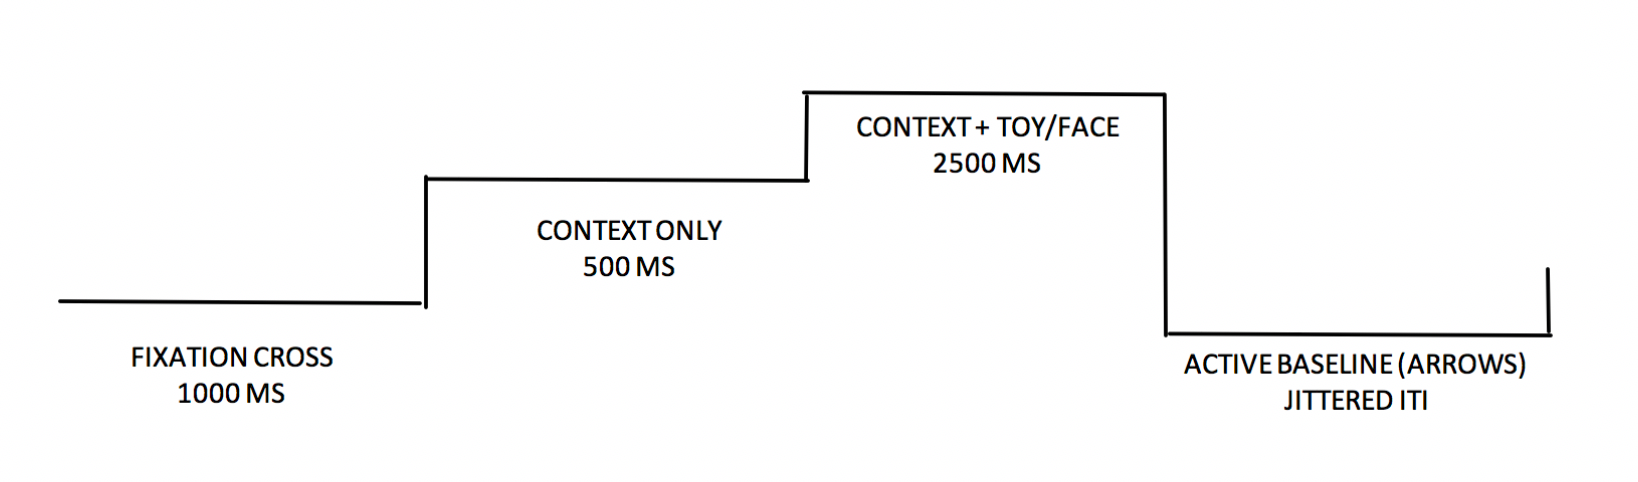
\includegraphics{images/information/measures/tasks/halloween/1.png}
\caption{}
\end{figure}

This is the basic structure of each block. First there is a fixation cross for 1 second, then a house will appear on the screen for 500ms, then the house+toy/sweets will appear on the screen for an addition 2.5 seconds (total of 3 seconds for the house and the house+toy/sweet, then there will be a baseline period that is jittered in length. The baseline is jittered in the MRI but it will be a fixed length of 1 seconds in the lab-based version of the task. In the MRI the active baseline will involve pressing buttons to indicate the direction of arrows on the screen, in the lab-based version of the task, it involves simply looking at a fixation dot.

There will be two blocks (day, and night). The day block is the emotionally neutral block, whereas the night block is the scary block. Each block has 20 trials (10 are the house + toy, 10 are the house + sweets). The toys/sweets that are paired with the houses are not counterbalanced, but the order of the blocks will be counterbalanced between participants (some will have day then night, and the rest will have night then day).

As an added layer to this task, we will not only pair an item with a house, but we will place it on top of the house in one quadrant. To encode a detailed associative memory, the individual will need to remember what item was paired with the house and then what quadrant it was in. For this test, a picture of a house will be shown along with 3 choices for which item matches with the house, one being correct and 2 serving as filler ``foils.'' The two ``foil'' options are items from other houses, so the child will have seen them before. Each item will both be a correct answer for the house it was initially paired with and a foil answer for two other houses throughout the trial. Additionally, the child will have to recall which quadrant the selected item was in on the house. The quadrants appear

For the recognition test there should be an equal number of foils as target items.

\begin{center}\rule{0.5\linewidth}{0.5pt}\end{center}

\hypertarget{characters-monstersaliens}{%
\subsubsection{Characters (monsters/aliens)}\label{characters-monstersaliens}}

\hypertarget{description-3}{%
\paragraph{Description}\label{description-3}}

Participants are instructed that their job in this game is to learn which ``character'' is right and which is wrong through trial-and-error. Participants are presented two stimuli side-by-side for 3500 milliseconds and indicate which character they choose by using the left and right arrow keys on the keyboard. Stimuli are presented in pairs AB, CD, EF (and their counterbalanced version BA, DC, FE). Stimuli A is correct in the AB/BA trials 80\% of the time. Stimuli C is correct in the CD/DC trials 70\% of the time. Stimuli E is correct in the EF/FE trials 60\% of the time. Stimuli are randomly shuffled and assigned a letter at the beginning of the task. For Mind, Brain, Body, the stimuli consisted of colorful monsters/aliens.

If participants choose ``correctly'' they will see a green check mark and hear ``ding'' sound. If they choose ``incorrectly'' they will see a red x mark and hear a ``horn'' sound. If they take longer than 3500 milliseconds to respond, they are shown a screen that says ``Too Slow''. All feedback is presented for 2000 milliseconds before moving on to the next trial. Stimuli pairs are presented 10 times each in random order in each block (total of 60 trials). PsychoPy tallies the correct and incorrect responses on a block-by-block basis. Participants move onto the test phase once they have reached a performance criterion (65\% accuracy for AB/BA trials, 60\% accuracy for CD/DC trials, 50\% accuracy for EF/FE trials). If participants do not reach criterion, they are automatically directed to the test after reaching a certain number of blocks (3 for children, 5 for adolescents).

During the test, participants are presented with all training pairs (AB/BA, CD/DC, EF/FE), and novel pairs including A and B (AC/CA, AD/DA, AE/EA, AF/FA, BC/CB, BD/DB, BE/EB, BF/FB). Test pairs are each presented 6 times. This section is untimed, and no feedback is provided.

\hypertarget{background-2}{%
\paragraph{Background}\label{background-2}}

The characters task assesses learning. It is a cognitive reinforcement learning task in which participants must learn to choose one stimulus over another through reinforcement. Participants can employ two strategies to learn the correct response---either they can learn to choose stimulus `A' or to avoid stimulus `B'. At test, these stimuli are paired with novel stimuli. If participants choose stimulus `A' over the novel stimulus, that is evidence of positive feedback learning. If participants choose the novel stimulus over stimulus `B', that is evidence of negative feedback learning. As a result, this task allows for direct comparison of sensitivity to these two types of learning \citep{frank_2004}.

\hypertarget{details-3}{%
\paragraph{Details}\label{details-3}}

PsychoPy parameters should be set to:

\begin{itemize}
\tightlist
\item
  10 trial\_loop nreps
\item
  3 test\_loop nreps
\item
  Maximum 5 block\_loops nreps (advances after criterion is met)
\end{itemize}

Physiology markers are set to:

\begin{itemize}
\tightlist
\item
  Channel 1 (28) - Train stimulus onset
\item
  Channel 2 (29) - Check
\item
  Channel 3 (30) - X
\item
  Channel 4 (31) - Miss
\item
  Channel 5 (32) - Test stimulus onset
\end{itemize}

Task based on original task by \citet{frank_2004}, re-programmed and adapted by Emily Towner and Ryan Burnell.

\begin{center}\rule{0.5\linewidth}{0.5pt}\end{center}

\hypertarget{discrimination-conditioning-extinction}{%
\subsubsection{Discrimination / Conditioning / Extinction}\label{discrimination-conditioning-extinction}}

\hypertarget{description-4}{%
\paragraph{Description}\label{description-4}}

Children and adolescent participants will take part in a visual perceptual threshold task. Participants will be shown visual stimuli (e.g., two black stripes at different orientations, or two Gabors with different levels of contrast) and asked to discriminate between them: ``which stripe is rotated more clockwise 1 or 2?'' for the stripes, or
``which picture is darker/clearer 1 or 2?'' for the Gabors. The magnitude of the difference between the two choices will be decreased after two correct choices, and increased after one correct choice, and will be continued until 6 wrong choices are made. The smallest magnitude where participants were able to correctly identify the stripe or Gabor in question is their Just Noticeable Difference (JND) threshold. The JND will be calculated before and after the threat learning task, and after the extinction task.

\hypertarget{details-4}{%
\paragraph{Details}\label{details-4}}

This task has two purposes.

\begin{enumerate}
\def\labelenumi{\arabic{enumi}.}
\tightlist
\item
  The first is to simply look at threat learning and extinction in children and adolescents across typical development and after adversity exposure. This has been done many times before, but we will also have children attached to an electrogastrogram (EGG - which is completely novel), GSR (sweat - which is the common measure), and heart rate (which is somewhat common but less so in the conditioning literature) while they and learning and extinguishing.
\item
  The second purpose of the task is to look at how conditioning and extinction affect perceptual thresholds. This is built from a large literature in adults showing that threat learning can lead to a broadening or narrowing of tuning curves following threat conditioning, depending on the specific parameters in place (more narrowing - i.e., better, occurs when a discriminatory conditioning procedure is employed and where the CS- and the CS+ and really different; more broadening occurs when the CS- and the CS+ are similar and when there is not explicit discriminative conditioning. We are going to employ a form of conditioning that has been shown to lead to perceptual broadening in adults.
\end{enumerate}

Past literature:
This paper by \citet{shalev_2018} demonstrates the effect we are trying to test in children/adolescents. They use an across sensory modality procedure (CSs = auditory, USs = visual) and between subjects design (control group = CS+ are positive/neutral, and experiments group where CS+ are negative) with pre/post perceptual tuning curves to determine the effect of threat learning on sensory discrimination.

The basic task structure:

\begin{figure}
\centering
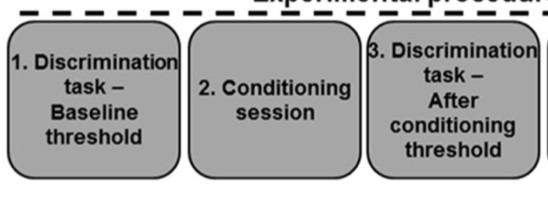
\includegraphics{images/information/measures/tasks/disc_cond_ext/1.png}
\caption{}
\end{figure}

The task and results:

They find that when the CS+ is paired with the aversive picture, people show a deterioration in their ability to discriminate the CS+ from tones that are similar to it, whereas they show very little change in their ability to discriminate the CS- from tones that are similar to it. They saw the same thing with gabors that differed in contrast (right) and lines that differed in orientation (left).

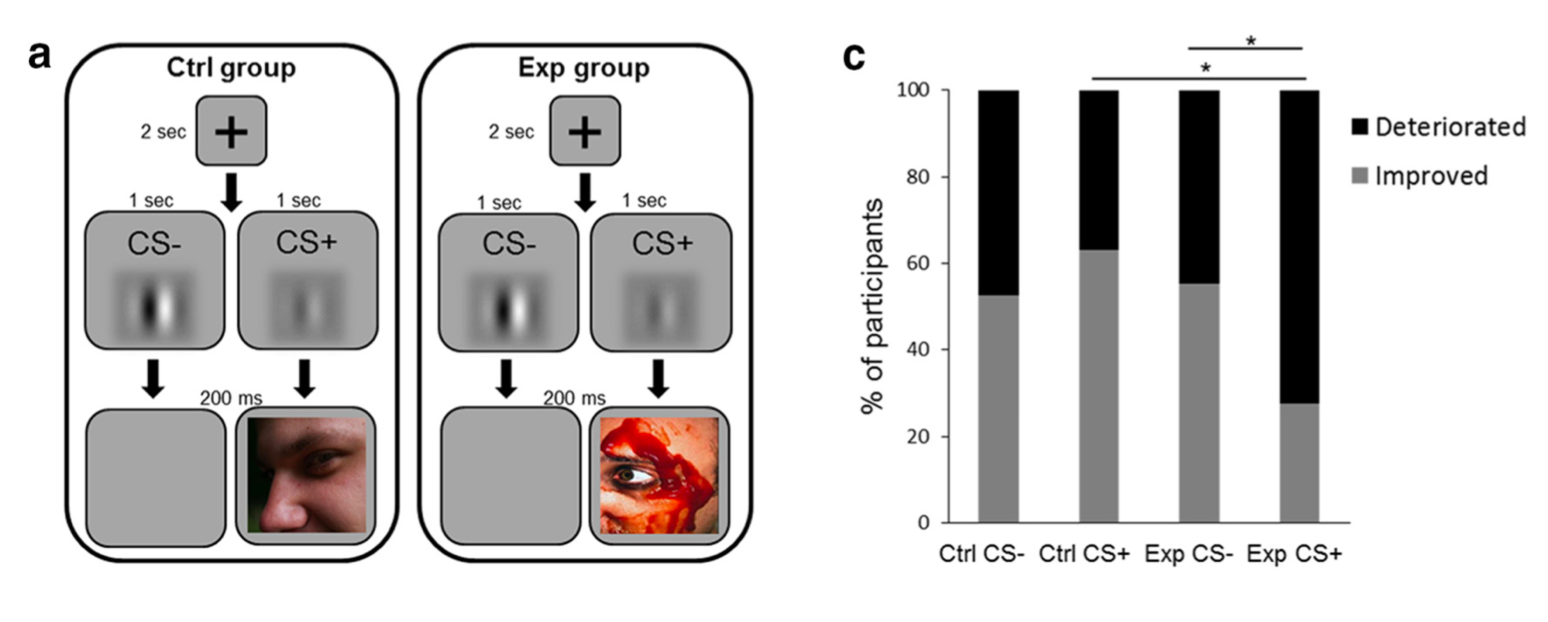
\includegraphics{images/information/measures/tasks/disc_cond_ext/2.png}
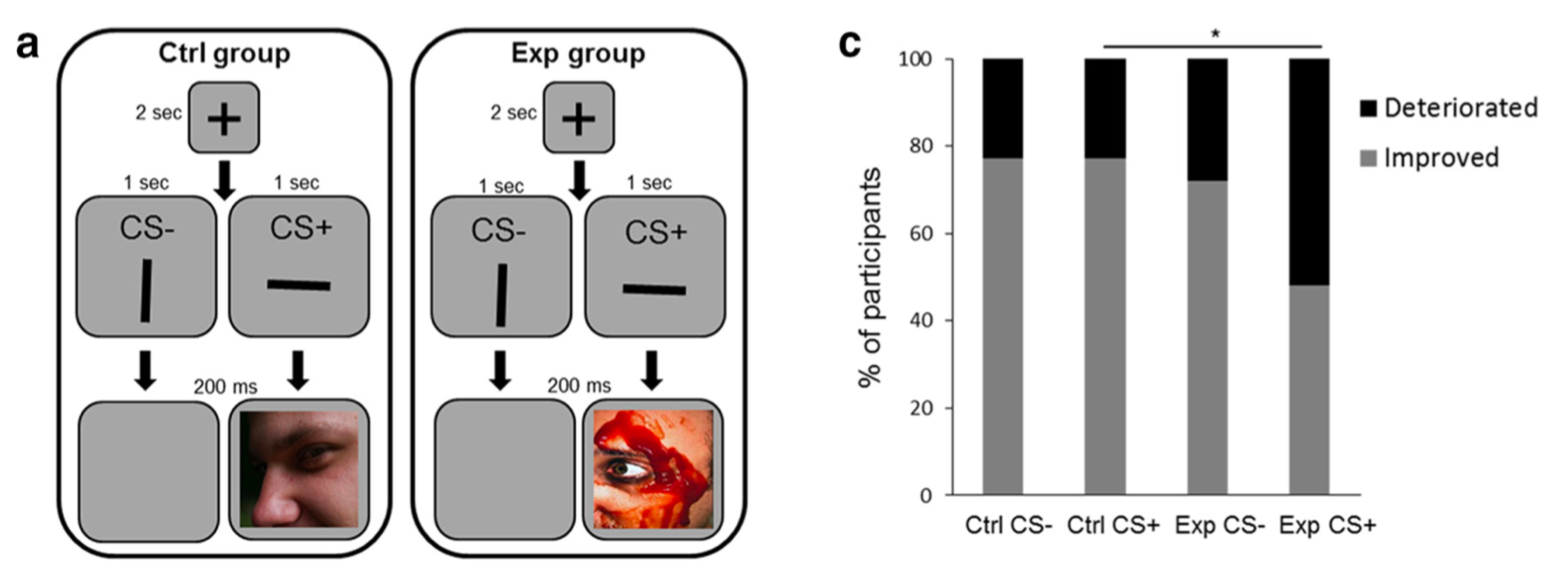
\includegraphics{images/information/measures/tasks/disc_cond_ext/3.png}
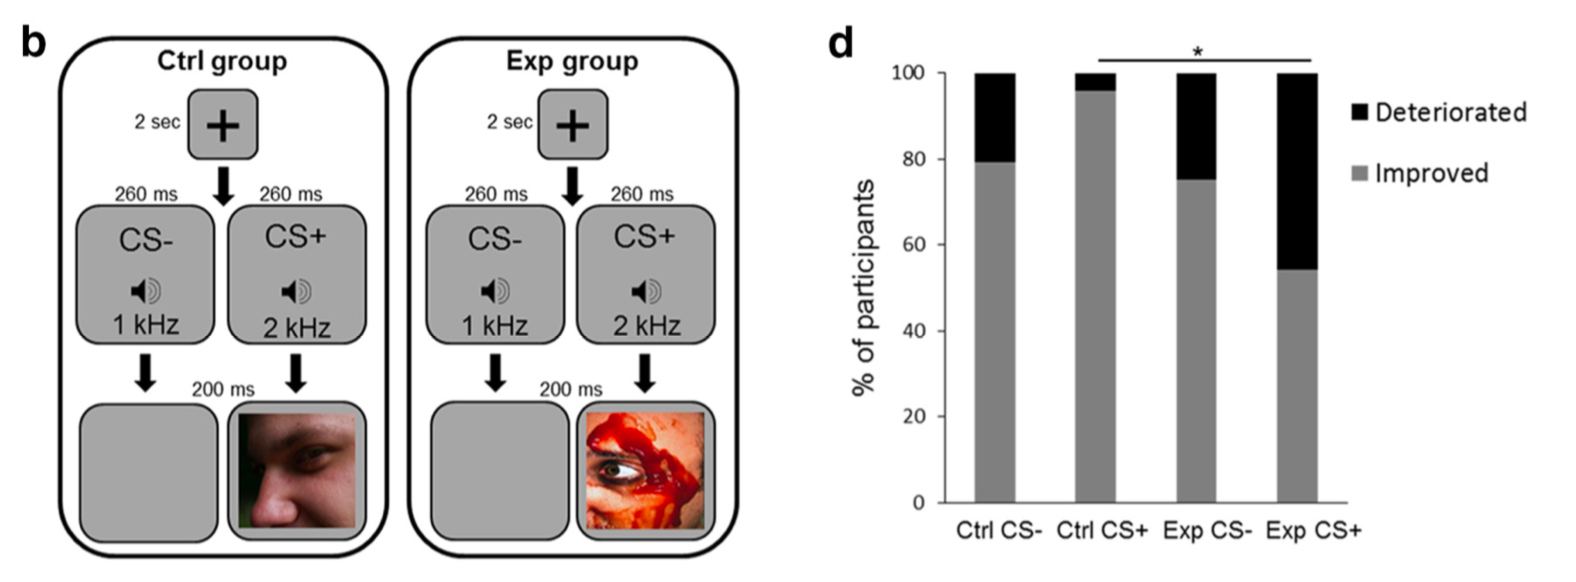
\includegraphics{images/information/measures/tasks/disc_cond_ext/4.png}

Current Task Structure:

We will use an approach where we pair aversive/pleasant noises (USs) with lines at different orientations (CSs). In the control group the noise will be pleasant or neutral. In the experimental group the noise will be aversive.

\begin{figure}
\centering
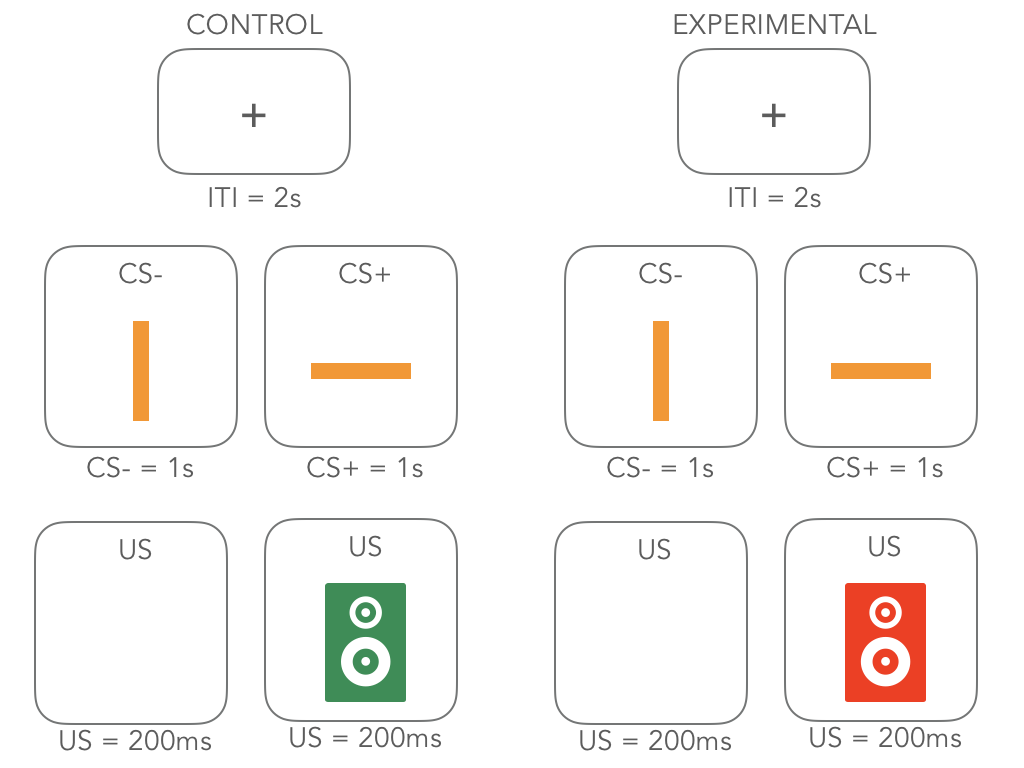
\includegraphics{images/information/measures/tasks/disc_cond_ext/5.png}
\caption{}
\end{figure}

The timeline of the task will be as follows:

\begin{figure}
\centering
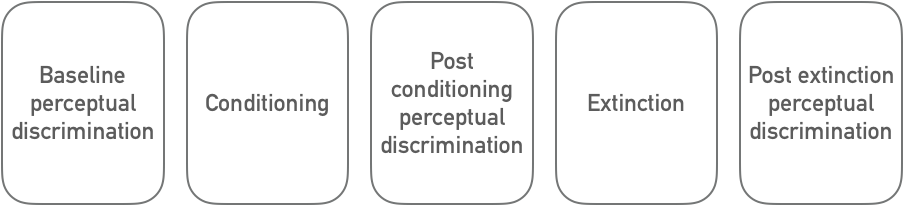
\includegraphics{images/information/measures/tasks/disc_cond_ext/6.png}
\caption{}
\end{figure}

\begin{itemize}
\tightlist
\item
  Number of trials was based on review of five papers \citetext{\citealp[ (56 trials)]{norrholm_2011}; \citealp[ (72 trials)]{norrholm_2006}; \citealp[ (32 trials)]{schiller_2013}; \citealp[ (34 trials)]{phelps_2004}; \citealp{jovanovic_2014}}.
\end{itemize}

The experimental protocol consisted of two phases: fear acquisition and extinction. The sessions were separated by 10 minutes. The acquisition phase consisted of 3 blocks, each with 3 CS+ trials, 3 CS− trials, and 3 noise alone (NA, no CS presented during startle probe) trials, for a total of 27 startle trials. Both CSs were colored shapes presented on a computer monitor for 6000 ms prior to the delivery of the startle probe, and co-terminated with the US 500 ms after the presentation of the startle stimulus. The CS+ was reinforced with the airblast 100\% of the time. The extinction phase consisted of 4 blocks with 3 trials of each type. The CSs were same as above, except that the CS+ was no longer paired with the airblast. In all phases of the experiment, inter-trial intervals will be randomized between 9 and 22 seconds.

\begin{longtable}[]{@{}ll@{}}
\toprule
\begin{minipage}[b]{0.12\columnwidth}\raggedright
Person\strut
\end{minipage} & \begin{minipage}[b]{0.82\columnwidth}\raggedright
Role\strut
\end{minipage}\tabularnewline
\midrule
\endhead
\begin{minipage}[t]{0.12\columnwidth}\raggedright
Bridget\strut
\end{minipage} & \begin{minipage}[t]{0.82\columnwidth}\raggedright
Developed concept\strut
\end{minipage}\tabularnewline
\begin{minipage}[t]{0.12\columnwidth}\raggedright
Psychopy tutorial\strut
\end{minipage} & \begin{minipage}[t]{0.82\columnwidth}\raggedright
The structure of the staircase\strut
\end{minipage}\tabularnewline
\begin{minipage}[t]{0.12\columnwidth}\raggedright
Paul Bloom\strut
\end{minipage} & \begin{minipage}[t]{0.82\columnwidth}\raggedright
Helped to adapt the staircase (changed from sequential to serial, centered stimuli, randomized order, added mask)\strut
\end{minipage}\tabularnewline
\begin{minipage}[t]{0.12\columnwidth}\raggedright
Emily Towner\strut
\end{minipage} & \begin{minipage}[t]{0.82\columnwidth}\raggedright
Building the task and completing the staircase\strut
\end{minipage}\tabularnewline
\bottomrule
\end{longtable}

\begin{center}\rule{0.5\linewidth}{0.5pt}\end{center}

\hypertarget{memory-generalization}{%
\subsubsection{Memory Generalization}\label{memory-generalization}}

\begin{center}\rule{0.5\linewidth}{0.5pt}\end{center}

\hypertarget{tests}{%
\subsection{Tests}\label{tests}}

\hypertarget{wasi}{%
\subsubsection{WASI}\label{wasi}}

\hypertarget{wiat}{%
\subsubsection{WIAT}\label{wiat}}

Wechsler Individual Achievement Test (WIAT) -- 4-85 years. Child/adolescent self-report. Domain assessed cognitive function. The WIAT is a comprehensive yet flexible measurement tool useful for achievement skills assessment, learning disability diagnosis, special education placement, and clinical appraisal for preschool children through adults. Norms allow for assessment of those from ages 4 to 85.

\begin{center}\rule{0.5\linewidth}{0.5pt}\end{center}

\hypertarget{measurements}{%
\subsection{Measurements}\label{measurements}}

\hypertarget{height-weight}{%
\subsubsection{Height \& Weight}\label{height-weight}}

Tri-ponderal mass (TPM) and body mass index (BMI) will be calculated using height and weight measurements. TPM/BMI has been related to the microbiome in past studies and is important to consider as a confounding variable in those analyses, as well as an outcome variable related to early adversity.

\hypertarget{waist-circumference}{%
\subsubsection{Waist Circumference}\label{waist-circumference}}

Waist circumference will be taken using measuring tape around the child and adolescent participant's waist. This will be an outcome measure related to effects of early adversity exposure on physical development.

\begin{center}\rule{0.5\linewidth}{0.5pt}\end{center}

\hypertarget{biological-samples}{%
\subsection{Biological Samples}\label{biological-samples}}

\hypertarget{hair-sample}{%
\subsubsection{Hair sample}\label{hair-sample}}

Child and adolescent participants will donate a head hair sample for the purpose of measuring average cortisol levels during the past month. To collect the sample, a few strands of hair behind the crown of the head will be cut close to the root. This method of collecting hair is not invasive and has been performed in babies \citep[32 weeks of age;][]{staufenbiel_2013}. Hair samples will never be used for genetic analysis.

\hypertarget{saliva-sample}{%
\subsubsection{Saliva sample}\label{saliva-sample}}

Saliva samples will be collected from child and adolescent participants in the lab using omnigene oral tubes (dnagenotek). Participants spit into a tube using a saliva collection kit. If participants are unable to spit, they will place small sterilized sponges in their mouths to collect the saliva. The sponges are then placed into the tube. After the cap of the tube is closed, it will break open a seal inside that releases a stabilizing solution into the tube which stabilizes the saliva. The saliva will be used to analyze bacteria in the oral cavity. The stabilization technique we use allows the saliva samples to remain at ambient temperature for several months. In batches, the saliva will sent to the processing facility. The samples will be labelled with participant ID codes only -- no personally identifying information. Only microbial DNA, not human DNA, is analyzed in these samples.

\hypertarget{blood-sample}{%
\subsubsection{Blood sample}\label{blood-sample}}

Dried Blood Spot Collection: Participants can opt into or out of participating in the dried blood spot collection (identified during the consent process). Those who opt into the blood spot collection will have one finger on their non¬dominant hand pricked in order to provide approximately ten drops of blood that will be placed on special filter paper cards and examined for circulating and molecular markers of inflammation. We will not collect blood from participants who are feeling ill or participants who take anticoagulants or blood thinners (e.g.~Heparin, Warfarin -- verified through medication checklist). Participants will be offered a Virtual Reality (VR) immersive headset to watch a video during the blood spot procedure. Previous studies have empirically demonstrated that VR can significantly reduce child/adolescent anxiety about blood spot/draw procedures. The trained researcher will massage the finger to be pricked to draw the blood circulation to that area, and will use BD Microtainer contact-activated lancets to make one prick the middle or ring finger on the non-dominant hand, disposing of the lancet in a bio¬hazard sharps container immediately. This procedure is similar to what children/adolescent may experience at a pediatrician visit. Five drops of blood are placed onto each of two Whatman 903 Proteinsaver cards (GE Healthcare Bio¬Sciences). After collection, the finger will be cleaned (with an alcohol swab), dried with gauze, and bandaged. Blood spot samples will be dried overnight, then closed, labeled with ID number and date, and stored in a small plastic bag with a desiccant pack. Bags are stored in -¬80 Celsius freezer until shipped for further processing. When shipped for further processing, the bags are placed in an insulated box with dry ice before being transported for analysis. Blood test results are not diagnostic and will not be shared with study participants. Risks of the procedure include temporary soreness at the site of the finger prick, or in very rare circumstances, infection. To minimize the risk of infection, we will follow sterile procedures, including the use of sterile, one-time-use lancets, sterile gauze/bandage, and alcohol wipes of the site. Blood will be collected in the Health Psychology Lab in Franz or in the SAND lab in Franz, which has a drape to maintain cleanliness of the collection area, a sharps container, as well as antibacterial cleaning materials to maintain cleanliness of the collection room. Experimenters performing the needle prick will wear gloves throughout the procedure and wear covered clothing as a safety precaution. The non¬dominant hand will be used and bandaged to avoid soreness from overuse at the site of the finger prick. If there is no blood, or not sufficient blood on the first finger prick, a second prick will be attempted on a different finger to avoid unnecessary discomfort. Experimenters performing the finger prick will be trained and certified in dried blood spot collection.

\hypertarget{stool-sample}{%
\subsubsection{Stool sample}\label{stool-sample}}

A stool sample will be collected from the child and adolescent participants in their home with the assistance of their parent using omnigene gut tubes (dnagenotek). Using a regular toilet, participants use the paper toilet hat to catch the stool. Participants will use a small sterile spatula to collect a pea sized amount of stool from the toilet hat and place it in the tube. After the lid is sealed, with the sample inside, the participant will shake the tube. A homogenization bead inside will break up the sample and cover all of the sample with a stabilizing liquid. The participant will place the stool sample into a biohazard bag, into a padded mailer, which will be returned to the lab through the registered post. The stabilization technique we use allows the stool samples to remain at ambient temperature for several weeks. Once the sample arrives at the lab, it will be placed into the locked -80 Celcius freezer until processing. Once all samples are collected we will pack the samples in dry ice and send to the processing facility. The samples will be labelled with participant ID codes only -- no personally identifying information. Only microbial DNA, not human DNA, is analyzed in these samples.

\begin{center}\rule{0.5\linewidth}{0.5pt}\end{center}

\hypertarget{questionnaires}{%
\subsection{Questionnaires}\label{questionnaires}}

\hypertarget{child}{%
\subsubsection{Child}\label{child}}

\begin{longtable}[]{@{}llllll@{}}
\toprule
\begin{minipage}[b]{0.18\columnwidth}\raggedright
Title\strut
\end{minipage} & \begin{minipage}[b]{0.18\columnwidth}\raggedright
Description\strut
\end{minipage} & \begin{minipage}[b]{0.15\columnwidth}\raggedright
Reference\strut
\end{minipage} & \begin{minipage}[b]{0.16\columnwidth}\raggedright
Respondent\strut
\end{minipage} & \begin{minipage}[b]{0.06\columnwidth}\raggedright
Wave\strut
\end{minipage} & \begin{minipage}[b]{0.10\columnwidth}\raggedright
Version\strut
\end{minipage}\tabularnewline
\midrule
\endhead
\begin{minipage}[t]{0.18\columnwidth}\raggedright
Alexithymia\strut
\end{minipage} & \begin{minipage}[t]{0.18\columnwidth}\raggedright
Child/adolescent self-report. Domain assessed: mental health/affective function. This questionnaire asks youth to endorse a number of items falling within three factors (1) Difficulty identifying feelings, (2) difficulty describing feelings, (3) externally oriented thinking.\strut
\end{minipage} & \begin{minipage}[t]{0.15\columnwidth}\raggedright
(Rieffe, Oosterveld, \& Terwogt, 2006)\strut
\end{minipage} & \begin{minipage}[t]{0.16\columnwidth}\raggedright
Wave 1, Wave 1 Online\strut
\end{minipage} & \begin{minipage}[t]{0.06\columnwidth}\raggedright
\strut
\end{minipage} & \begin{minipage}[t]{0.10\columnwidth}\raggedright
\strut
\end{minipage}\tabularnewline
\begin{minipage}[t]{0.18\columnwidth}\raggedright
Children's Perception of Interparental Conflict Scale (cpic)-- 6-18 years\strut
\end{minipage} & \begin{minipage}[t]{0.18\columnwidth}\raggedright
Child/adolescent self-report. Domains assessed: parenting and family structure. The CPIC assesses children's/adolescent's experience of parental conflict, including subscales (Conflict Properties, Threat, Self-Blame).\strut
\end{minipage} & \begin{minipage}[t]{0.15\columnwidth}\raggedright
(ABC, XXXX)\strut
\end{minipage} & \begin{minipage}[t]{0.16\columnwidth}\raggedright
Wave 1, Wave 1 Online\strut
\end{minipage} & \begin{minipage}[t]{0.06\columnwidth}\raggedright
\strut
\end{minipage} & \begin{minipage}[t]{0.10\columnwidth}\raggedright
\strut
\end{minipage}\tabularnewline
\begin{minipage}[t]{0.18\columnwidth}\raggedright
Child Somatization Symptom Inventory (cssi)-- 6-17 years\strut
\end{minipage} & \begin{minipage}[t]{0.18\columnwidth}\raggedright
Child/adolescent self-report. Parent report for children under 8 years. Domain assessed: physical symptoms. The CSSI assesses a variety of nonspecific somatic symptoms.\strut
\end{minipage} & \begin{minipage}[t]{0.15\columnwidth}\raggedright
(ABC, XXXX)\strut
\end{minipage} & \begin{minipage}[t]{0.16\columnwidth}\raggedright
Wave 1, Wave 1 Online\strut
\end{minipage} & \begin{minipage}[t]{0.06\columnwidth}\raggedright
\strut
\end{minipage} & \begin{minipage}[t]{0.10\columnwidth}\raggedright
\strut
\end{minipage}\tabularnewline
\begin{minipage}[t]{0.18\columnwidth}\raggedright
Security Scale (ss) -- 8-18 years\strut
\end{minipage} & \begin{minipage}[t]{0.18\columnwidth}\raggedright
Child/adolescent self-report. Domain assessed: attachment. This measure asks children/adolescents to endorse statements about their feelings towards their parents (in the positive or negative) and how much each endorsed statement is characteristic of them. Statements assess domains of being able to rely on parents in times of need, feelings of closeness with parent etc.\strut
\end{minipage} & \begin{minipage}[t]{0.15\columnwidth}\raggedright
(ABC, XXXX)\strut
\end{minipage} & \begin{minipage}[t]{0.16\columnwidth}\raggedright
Wave 1, Wave 1 Online\strut
\end{minipage} & \begin{minipage}[t]{0.06\columnwidth}\raggedright
\strut
\end{minipage} & \begin{minipage}[t]{0.10\columnwidth}\raggedright
\strut
\end{minipage}\tabularnewline
\begin{minipage}[t]{0.18\columnwidth}\raggedright
Benevolent Childhood Experiences Scale- Revised (bce)\strut
\end{minipage} & \begin{minipage}[t]{0.18\columnwidth}\raggedright
Child/adolescent self-report. Domain assessed: benevolent childhood experiences. This child/adolescent self-report questionnaire consists of 10 items used to identify favorable childhood experiences, with regards to potential child adversity.\strut
\end{minipage} & \begin{minipage}[t]{0.15\columnwidth}\raggedright
(ABC, XXXX)\strut
\end{minipage} & \begin{minipage}[t]{0.16\columnwidth}\raggedright
Wave 1 Online\strut
\end{minipage} & \begin{minipage}[t]{0.06\columnwidth}\raggedright
\strut
\end{minipage} & \begin{minipage}[t]{0.10\columnwidth}\raggedright
\strut
\end{minipage}\tabularnewline
\bottomrule
\end{longtable}

Notes:

Attention checks were embedded in several child questionnaires beginning with MBB online.

\begin{itemize}
\tightlist
\item
  attention\_check\_1 (ss)
\item
  attention\_check\_2 (cpic)
\item
  attention\_check\_3 (alexithymia)
\item
  attention\_check\_4 (bce)
\item
  attention\_check\_5 (cssi)
\end{itemize}

\begin{center}\rule{0.5\linewidth}{0.5pt}\end{center}

\hypertarget{parent}{%
\subsubsection{Parent}\label{parent}}

\hypertarget{parent-self}{%
\paragraph{Parent Self}\label{parent-self}}

\begin{longtable}[]{@{}llllll@{}}
\toprule
\begin{minipage}[b]{0.18\columnwidth}\raggedright
Title\strut
\end{minipage} & \begin{minipage}[b]{0.18\columnwidth}\raggedright
Description\strut
\end{minipage} & \begin{minipage}[b]{0.15\columnwidth}\raggedright
Reference\strut
\end{minipage} & \begin{minipage}[b]{0.16\columnwidth}\raggedright
Respondent\strut
\end{minipage} & \begin{minipage}[b]{0.06\columnwidth}\raggedright
Wave\strut
\end{minipage} & \begin{minipage}[b]{0.10\columnwidth}\raggedright
Version\strut
\end{minipage}\tabularnewline
\midrule
\endhead
\begin{minipage}[t]{0.18\columnwidth}\raggedright
Beck Depression Inventory -- II (bdi\_ii)\strut
\end{minipage} & \begin{minipage}[t]{0.18\columnwidth}\raggedright
Mental health/affective functioning. Developed for the assessment of symptoms corresponding to criteria for diagnosing depressive disorders listed in the DSM IV.\strut
\end{minipage} & \begin{minipage}[t]{0.15\columnwidth}\raggedright
(ABC, XXXX)\strut
\end{minipage} & \begin{minipage}[t]{0.16\columnwidth}\raggedright
Parents (self report)\strut
\end{minipage} & \begin{minipage}[t]{0.06\columnwidth}\raggedright
Wave 1, Wave 1 Online\strut
\end{minipage} & \begin{minipage}[t]{0.10\columnwidth}\raggedright
\strut
\end{minipage}\tabularnewline
\begin{minipage}[t]{0.18\columnwidth}\raggedright
COVID-19 Objective Questionnaire (covid\_objective)\strut
\end{minipage} & \begin{minipage}[t]{0.18\columnwidth}\raggedright
COVID-19 objective measures. This questionnaire consists of 12 items to identify health changes and lifestyle changes made From the impacts of the COVID-19 outbreak.\strut
\end{minipage} & \begin{minipage}[t]{0.15\columnwidth}\raggedright
(ABC, XXXX)\strut
\end{minipage} & \begin{minipage}[t]{0.16\columnwidth}\raggedright
Parents (self report)\strut
\end{minipage} & \begin{minipage}[t]{0.06\columnwidth}\raggedright
Wave 1 Online\strut
\end{minipage} & \begin{minipage}[t]{0.10\columnwidth}\raggedright
\strut
\end{minipage}\tabularnewline
\bottomrule
\end{longtable}

\hypertarget{parent-proxy}{%
\paragraph{Parent Proxy}\label{parent-proxy}}

\begin{longtable}[]{@{}llllll@{}}
\toprule
\begin{minipage}[b]{0.18\columnwidth}\raggedright
Title\strut
\end{minipage} & \begin{minipage}[b]{0.18\columnwidth}\raggedright
Description\strut
\end{minipage} & \begin{minipage}[b]{0.15\columnwidth}\raggedright
Reference\strut
\end{minipage} & \begin{minipage}[b]{0.16\columnwidth}\raggedright
Respondent\strut
\end{minipage} & \begin{minipage}[b]{0.06\columnwidth}\raggedright
Wave\strut
\end{minipage} & \begin{minipage}[b]{0.10\columnwidth}\raggedright
Version\strut
\end{minipage}\tabularnewline
\midrule
\endhead
\begin{minipage}[t]{0.18\columnwidth}\raggedright
Demographic Questionnaire\strut
\end{minipage} & \begin{minipage}[t]{0.18\columnwidth}\raggedright
Demographics. The project developed questionnaire asks parents about their household income, their own and their child's/adolescent's race/ethnicity, the parent age, education, and marital status, and contact details.\strut
\end{minipage} & \begin{minipage}[t]{0.15\columnwidth}\raggedright
(ABC, XXXX)\strut
\end{minipage} & \begin{minipage}[t]{0.16\columnwidth}\raggedright
Parents (proxy)\strut
\end{minipage} & \begin{minipage}[t]{0.06\columnwidth}\raggedright
Wave 1, Wave 1 Online\strut
\end{minipage} & \begin{minipage}[t]{0.10\columnwidth}\raggedright
\strut
\end{minipage}\tabularnewline
\begin{minipage}[t]{0.18\columnwidth}\raggedright
Pediatric Quality of Life - Gastrointestinal (pedsql\_gi)\strut
\end{minipage} & \begin{minipage}[t]{0.18\columnwidth}\raggedright
Physical symptoms. The PedsQL Gastrointestinal Symptoms Scale will be administered. These questionnaires are designed to assess the incidence of gastrointestinal symptoms in youth.\strut
\end{minipage} & \begin{minipage}[t]{0.15\columnwidth}\raggedright
(ABC, XXXX)\strut
\end{minipage} & \begin{minipage}[t]{0.16\columnwidth}\raggedright
Parents (proxy)\strut
\end{minipage} & \begin{minipage}[t]{0.06\columnwidth}\raggedright
Wave 1, Wave 1 Online\strut
\end{minipage} & \begin{minipage}[t]{0.10\columnwidth}\raggedright
\strut
\end{minipage}\tabularnewline
\begin{minipage}[t]{0.18\columnwidth}\raggedright
Pediatric Quality of Life - Well Being (pedsql\_wb)\strut
\end{minipage} & \begin{minipage}[t]{0.18\columnwidth}\raggedright
Physical symptoms. The PedsQL General Wellbeing Scale will be administered. These questionnaires are designed to assess general feelings of wellbeing in youth.\strut
\end{minipage} & \begin{minipage}[t]{0.15\columnwidth}\raggedright
(ABC, XXXX)\strut
\end{minipage} & \begin{minipage}[t]{0.16\columnwidth}\raggedright
Parents (proxy)\strut
\end{minipage} & \begin{minipage}[t]{0.06\columnwidth}\raggedright
Wave 1, Wave 1 Online\strut
\end{minipage} & \begin{minipage}[t]{0.10\columnwidth}\raggedright
\strut
\end{minipage}\tabularnewline
\begin{minipage}[t]{0.18\columnwidth}\raggedright
Pediatric Quality of Life (pedsql\_f)\strut
\end{minipage} & \begin{minipage}[t]{0.18\columnwidth}\raggedright
Physical symptoms. The PedsQL Multidimensional Fatigue Scale will be administered. These questionnaires are designed to assess the incidence of fatigue symptoms in youth.\strut
\end{minipage} & \begin{minipage}[t]{0.15\columnwidth}\raggedright
(ABC, XXXX)\strut
\end{minipage} & \begin{minipage}[t]{0.16\columnwidth}\raggedright
Parents (proxy)\strut
\end{minipage} & \begin{minipage}[t]{0.06\columnwidth}\raggedright
Wave 1, Wave 1 Online\strut
\end{minipage} & \begin{minipage}[t]{0.10\columnwidth}\raggedright
\strut
\end{minipage}\tabularnewline
\begin{minipage}[t]{0.18\columnwidth}\raggedright
Revised Evaluation of Activity Survey in Youth (easy)\strut
\end{minipage} & \begin{minipage}[t]{0.18\columnwidth}\raggedright
Physical symptoms. The EASY asks parents to rate how physically active their child/adolescent has been during COVID-19.\strut
\end{minipage} & \begin{minipage}[t]{0.15\columnwidth}\raggedright
(ABC, XXXX)\strut
\end{minipage} & \begin{minipage}[t]{0.16\columnwidth}\raggedright
Parents (proxy)\strut
\end{minipage} & \begin{minipage}[t]{0.06\columnwidth}\raggedright
Wave 1, Wave 1 Online\strut
\end{minipage} & \begin{minipage}[t]{0.10\columnwidth}\raggedright
\strut
\end{minipage}\tabularnewline
\begin{minipage}[t]{0.18\columnwidth}\raggedright
Revised Traumatic Events Screening Inventory (tesi)\strut
\end{minipage} & \begin{minipage}[t]{0.18\columnwidth}\raggedright
Caregiving adversity. The TESI-C assesses a child's/adolescent's experience of a variety of potential traumatic events including physical/sexual abuse and neglect.\strut
\end{minipage} & \begin{minipage}[t]{0.15\columnwidth}\raggedright
(ABC, XXXX)\strut
\end{minipage} & \begin{minipage}[t]{0.16\columnwidth}\raggedright
Parents (proxy) Wave 1, Wave 1 Online\strut
\end{minipage} & \begin{minipage}[t]{0.06\columnwidth}\raggedright
\strut
\end{minipage} & \begin{minipage}[t]{0.10\columnwidth}\raggedright
\strut
\end{minipage}\tabularnewline
\begin{minipage}[t]{0.18\columnwidth}\raggedright
Child Behavior Checklist (cbcl)\strut
\end{minipage} & \begin{minipage}[t]{0.18\columnwidth}\raggedright
Mental health/affective function. Assesses behavioral competency and behavioral problems in children and adolescents within the past six months. The following syndrome scales are assessed: anxious/depressed, withdrawn/depressed, somatic complains, social problems, thought problems, rule-breaking behavior, and aggressive behavior.\strut
\end{minipage} & \begin{minipage}[t]{0.15\columnwidth}\raggedright
(ABC, XXXX)\strut
\end{minipage} & \begin{minipage}[t]{0.16\columnwidth}\raggedright
Parents (proxy)\strut
\end{minipage} & \begin{minipage}[t]{0.06\columnwidth}\raggedright
Wave 1, Wave 1 Online\strut
\end{minipage} & \begin{minipage}[t]{0.10\columnwidth}\raggedright
\strut
\end{minipage}\tabularnewline
\begin{minipage}[t]{0.18\columnwidth}\raggedright
Child Sleep Habits Questionnaire (csqh)\strut
\end{minipage} & \begin{minipage}[t]{0.18\columnwidth}\raggedright
Sleep. Multidimensional sleep assessment including sleeping difficulties, behavioral problems around sleep etc.\strut
\end{minipage} & \begin{minipage}[t]{0.15\columnwidth}\raggedright
(ABC, XXXX)\strut
\end{minipage} & \begin{minipage}[t]{0.16\columnwidth}\raggedright
Parents (proxy)\strut
\end{minipage} & \begin{minipage}[t]{0.06\columnwidth}\raggedright
Wave 1, Wave 1 Online\strut
\end{minipage} & \begin{minipage}[t]{0.10\columnwidth}\raggedright
\strut
\end{minipage}\tabularnewline
\begin{minipage}[t]{0.18\columnwidth}\raggedright
Microbiome metadata questionnaire (mb\_metadata)\strut
\end{minipage} & \begin{minipage}[t]{0.18\columnwidth}\raggedright
Microbiome metadata. This study developed questionnaire asks parents to report on a number of variables known to influence the microbiome, including whether their child/adolescent was born prematurely, mode of birth, pre- or post-natal antibiotic usage, pets in the home, country of birth, breast or bottle feeding, special diets (e.g., vegetarianism or dairy free).\strut
\end{minipage} & \begin{minipage}[t]{0.15\columnwidth}\raggedright
(ABC, XXXX)\strut
\end{minipage} & \begin{minipage}[t]{0.16\columnwidth}\raggedright
Parents (proxy)\strut
\end{minipage} & \begin{minipage}[t]{0.06\columnwidth}\raggedright
Wave 1, Wave 1 Online\strut
\end{minipage} & \begin{minipage}[t]{0.10\columnwidth}\raggedright
\strut
\end{minipage}\tabularnewline
\begin{minipage}[t]{0.18\columnwidth}\raggedright
Medication Checklist (med\_check)\strut
\end{minipage} & \begin{minipage}[t]{0.18\columnwidth}\raggedright
Parents are asked to list all medications that their children/adolescents are on. This information is used as a covariate in analyses of brain, microbiome, and biomarker data, as different medications can affect the readouts from these assays/analyses.\strut
\end{minipage} & \begin{minipage}[t]{0.15\columnwidth}\raggedright
(ABC, XXXX)\strut
\end{minipage} & \begin{minipage}[t]{0.16\columnwidth}\raggedright
Parents (proxy)\strut
\end{minipage} & \begin{minipage}[t]{0.06\columnwidth}\raggedright
Wave 1, Wave 1 Online\strut
\end{minipage} & \begin{minipage}[t]{0.10\columnwidth}\raggedright
\strut
\end{minipage}\tabularnewline
\begin{minipage}[t]{0.18\columnwidth}\raggedright
Petersen Physical Development Scales (pds)\strut
\end{minipage} & \begin{minipage}[t]{0.18\columnwidth}\raggedright
The Peterson Puberty Scale is an adaptation of an interview-based puberty-rating scale by Petersen, and includes scores for each of five items rating physical development, an overall maturation measure, and a categorical maturation score. It is designed to be non-invasive, not requiring the use of pictures.\strut
\end{minipage} & \begin{minipage}[t]{0.15\columnwidth}\raggedright
(ABC, XXXX)\strut
\end{minipage} & \begin{minipage}[t]{0.16\columnwidth}\raggedright
Parents (proxy)\strut
\end{minipage} & \begin{minipage}[t]{0.06\columnwidth}\raggedright
Wave 1, Wave 1 Online\strut
\end{minipage} & \begin{minipage}[t]{0.10\columnwidth}\raggedright
Male and female\strut
\end{minipage}\tabularnewline
\begin{minipage}[t]{0.18\columnwidth}\raggedright
Digestive Health and Wellbeing Survey (dhws)\strut
\end{minipage} & \begin{minipage}[t]{0.18\columnwidth}\raggedright
This survey asks parents to endorse whether a doctor has ever diagnosed their child/adolescent with a range of allergic and autoimmune conditions.\strut
\end{minipage} & \begin{minipage}[t]{0.15\columnwidth}\raggedright
(ABC, XXXX)\strut
\end{minipage} & \begin{minipage}[t]{0.16\columnwidth}\raggedright
Parents (proxy)\strut
\end{minipage} & \begin{minipage}[t]{0.06\columnwidth}\raggedright
Wave 1, Wave 1 Online\strut
\end{minipage} & \begin{minipage}[t]{0.10\columnwidth}\raggedright
\strut
\end{minipage}\tabularnewline
\begin{minipage}[t]{0.18\columnwidth}\raggedright
Hair-Care Practice Questionnaire (hpq).\strut
\end{minipage} & \begin{minipage}[t]{0.18\columnwidth}\raggedright
This questionnaire consists of 9 items for parents to indicate their child/adolescent's hair care practices for information relevant to the hair sample.\strut
\end{minipage} & \begin{minipage}[t]{0.15\columnwidth}\raggedright
(ABC, XXXX)\strut
\end{minipage} & \begin{minipage}[t]{0.16\columnwidth}\raggedright
Parents (proxy){[}for Wave 1 children under 10, for Wave 1 online all children{]}\strut
\end{minipage} & \begin{minipage}[t]{0.06\columnwidth}\raggedright
Wave 1, Wave 1 Online\strut
\end{minipage} & \begin{minipage}[t]{0.10\columnwidth}\raggedright
\strut
\end{minipage}\tabularnewline
\begin{minipage}[t]{0.18\columnwidth}\raggedright
Child Somatization Symptom Inventory (cssi)\strut
\end{minipage} & \begin{minipage}[t]{0.18\columnwidth}\raggedright
The CSSI assesses a variety of nonspecific somatic symptoms.\strut
\end{minipage} & \begin{minipage}[t]{0.15\columnwidth}\raggedright
(ABC, XXXX)\strut
\end{minipage} & \begin{minipage}[t]{0.16\columnwidth}\raggedright
Parents (proxy){[}children \textless{} 8 years{]}\strut
\end{minipage} & \begin{minipage}[t]{0.06\columnwidth}\raggedright
Wave 1, Wave 1 Online\strut
\end{minipage} & \begin{minipage}[t]{0.10\columnwidth}\raggedright
\strut
\end{minipage}\tabularnewline
\begin{minipage}[t]{0.18\columnwidth}\raggedright
Foster Care Inventory (fci)\strut
\end{minipage} & \begin{minipage}[t]{0.18\columnwidth}\raggedright
This instrument was made for the current study and assesses the number of foster care placements and care history.\strut
\end{minipage} & \begin{minipage}[t]{0.15\columnwidth}\raggedright
(ABC, XXXX)\strut
\end{minipage} & \begin{minipage}[t]{0.16\columnwidth}\raggedright
Parents (proxy){[}adopted only{]}\strut
\end{minipage} & \begin{minipage}[t]{0.06\columnwidth}\raggedright
Wave 1, Wave 1 Online\strut
\end{minipage} & \begin{minipage}[t]{0.10\columnwidth}\raggedright
\strut
\end{minipage}\tabularnewline
\begin{minipage}[t]{0.18\columnwidth}\raggedright
International Adoption Inventory (iai)\strut
\end{minipage} & \begin{minipage}[t]{0.18\columnwidth}\raggedright
This instrument was made for the study and asks parents of internationally adopted youth about the quality of institution and details of the adoption process.\strut
\end{minipage} & \begin{minipage}[t]{0.15\columnwidth}\raggedright
(ABC, XXXX)\strut
\end{minipage} & \begin{minipage}[t]{0.16\columnwidth}\raggedright
Parents (proxy){[}adopted only{]}\strut
\end{minipage} & \begin{minipage}[t]{0.06\columnwidth}\raggedright
\strut
\end{minipage} & \begin{minipage}[t]{0.10\columnwidth}\raggedright
\strut
\end{minipage}\tabularnewline
\begin{minipage}[t]{0.18\columnwidth}\raggedright
Financial Support Questionnaire (financial)\strut
\end{minipage} & \begin{minipage}[t]{0.18\columnwidth}\raggedright
The project developed financial support questionnaire assesses public assistance received, and health insurance information. All questions on this assessment (as with all assessments) will have an option not to disclose this information.\strut
\end{minipage} & \begin{minipage}[t]{0.15\columnwidth}\raggedright
(ABC, XXXX)\strut
\end{minipage} & \begin{minipage}[t]{0.16\columnwidth}\raggedright
Parents (proxy)\strut
\end{minipage} & \begin{minipage}[t]{0.06\columnwidth}\raggedright
Wave 1, Wave 1 Online\strut
\end{minipage} & \begin{minipage}[t]{0.10\columnwidth}\raggedright
\strut
\end{minipage}\tabularnewline
\begin{minipage}[t]{0.18\columnwidth}\raggedright
Bristol Stool Scale (bss)\strut
\end{minipage} & \begin{minipage}[t]{0.18\columnwidth}\raggedright
Stool sample short questionnaire: After collecting the stool sample, participants will be asked to indicate on a short questionnaire whether they were feeling ill on the day the sample was collected, what time the sample was collected, and consistency of stool. They will also be asked if their diet on the day of sample collection was typical.\strut
\end{minipage} & \begin{minipage}[t]{0.15\columnwidth}\raggedright
(ABC, XXXX)\strut
\end{minipage} & \begin{minipage}[t]{0.16\columnwidth}\raggedright
\strut
\end{minipage} & \begin{minipage}[t]{0.06\columnwidth}\raggedright
Parent (proxy)\strut
\end{minipage} & \begin{minipage}[t]{0.10\columnwidth}\raggedright
Wave 1, Wave 1 Online\strut
\end{minipage}\tabularnewline
\begin{minipage}[t]{0.18\columnwidth}\raggedright
COVID-19 Objective Questionnaire (covid\_objective)\strut
\end{minipage} & \begin{minipage}[t]{0.18\columnwidth}\raggedright
COVID-19 objective measures. This questionnaire consists of 12 items to identify health changes and lifestyle changes made From the impacts of the COVID-19 outbreak.\strut
\end{minipage} & \begin{minipage}[t]{0.15\columnwidth}\raggedright
(ABC, XXXX)\strut
\end{minipage} & \begin{minipage}[t]{0.16\columnwidth}\raggedright
Parents (proxy)\strut
\end{minipage} & \begin{minipage}[t]{0.06\columnwidth}\raggedright
\strut
\end{minipage} & \begin{minipage}[t]{0.10\columnwidth}\raggedright
\strut
\end{minipage}\tabularnewline
\begin{minipage}[t]{0.18\columnwidth}\raggedright
Parenting Stress (parenting\_stress)\strut
\end{minipage} & \begin{minipage}[t]{0.18\columnwidth}\raggedright
Designed to evaluate the magnitude of stress in the parent-child system, focusing on three major domains of stress: 1) child/adolescent characteristics, 2) parent characteristics, and 3) situational/demographic life stress. Revised questionnaire focuses on stress in the context of COVID-19.\strut
\end{minipage} & \begin{minipage}[t]{0.15\columnwidth}\raggedright
(ABC, XXXX)\strut
\end{minipage} & \begin{minipage}[t]{0.16\columnwidth}\raggedright
Parents (proxy)\strut
\end{minipage} & \begin{minipage}[t]{0.06\columnwidth}\raggedright
Wave 1 online\strut
\end{minipage} & \begin{minipage}[t]{0.10\columnwidth}\raggedright
\strut
\end{minipage}\tabularnewline
\bottomrule
\end{longtable}

\begin{center}\rule{0.5\linewidth}{0.5pt}\end{center}

\hypertarget{qualitative}{%
\subsubsection{Qualitative}\label{qualitative}}

\hypertarget{covid-19-written-responses}{%
\paragraph{COVID-19 Written Responses}\label{covid-19-written-responses}}

\begin{longtable}[]{@{}llllll@{}}
\toprule
\begin{minipage}[b]{0.18\columnwidth}\raggedright
Title\strut
\end{minipage} & \begin{minipage}[b]{0.18\columnwidth}\raggedright
Description\strut
\end{minipage} & \begin{minipage}[b]{0.15\columnwidth}\raggedright
Reference\strut
\end{minipage} & \begin{minipage}[b]{0.16\columnwidth}\raggedright
Respondent\strut
\end{minipage} & \begin{minipage}[b]{0.06\columnwidth}\raggedright
Wave\strut
\end{minipage} & \begin{minipage}[b]{0.10\columnwidth}\raggedright
Version\strut
\end{minipage}\tabularnewline
\midrule
\endhead
\begin{minipage}[t]{0.18\columnwidth}\raggedright
COVID-19 Written Response (written\_response\_parentself)\strut
\end{minipage} & \begin{minipage}[t]{0.18\columnwidth}\raggedright
Domain assessed: Emotional impacts of COVID-19. This self-report measure consists of one long-form qualitative response, prompting a parent to write continuously for five minutes about the impacts of COVID-19 on their life and family. This qualitative response was adapted from previous prompts in writing about emotional experiences, and seeks to assess the emotional and behavioral impacts of the Pandemic on children and families.\strut
\end{minipage} & \begin{minipage}[t]{0.15\columnwidth}\raggedright
(ABC, XXXX)\strut
\end{minipage} & \begin{minipage}[t]{0.16\columnwidth}\raggedright
Parents (self report)\strut
\end{minipage} & \begin{minipage}[t]{0.06\columnwidth}\raggedright
Wave 1 Online {[}optional{]}\strut
\end{minipage} & \begin{minipage}[t]{0.10\columnwidth}\raggedright
\strut
\end{minipage}\tabularnewline
\begin{minipage}[t]{0.18\columnwidth}\raggedright
COVID-19 Written Response (written\_response)\strut
\end{minipage} & \begin{minipage}[t]{0.18\columnwidth}\raggedright
Domain assessed: Emotional impacts of COVID-19. This self-report measure consists of one long-form qualitative response, prompting a child to write continuously for five minutes about the impacts of COVID-19 on their life and family (for children who cannot write or do not feel comfortable writing, children can dictate and parent can write). This qualitative response was adapted from previous prompts in writing about emotional experiences, and seeks to assess the emotional and behavioral impacts of the Pandemic on children and families.\strut
\end{minipage} & \begin{minipage}[t]{0.15\columnwidth}\raggedright
(ABC, XXXX)\strut
\end{minipage} & \begin{minipage}[t]{0.16\columnwidth}\raggedright
Children\strut
\end{minipage} & \begin{minipage}[t]{0.06\columnwidth}\raggedright
Wave 1 Online {[}optional{]}\strut
\end{minipage} & \begin{minipage}[t]{0.10\columnwidth}\raggedright
\strut
\end{minipage}\tabularnewline
\bottomrule
\end{longtable}

\begin{center}\rule{0.5\linewidth}{0.5pt}\end{center}

\hypertarget{wave-1}{%
\chapter{Wave 1}\label{wave-1}}

\hypertarget{checklists}{%
\section{Checklists}\label{checklists}}

\begin{center}\rule{0.5\linewidth}{0.5pt}\end{center}

\hypertarget{checklist---initial}{%
\subsection{Checklist - Initial}\label{checklist---initial}}

\textbf{Scheduling and Confirmation}

\begin{itemize}
\tightlist
\item
  Schedule lab session
\item
  Send confirmation email (in templates)

  \begin{itemize}
  \tightlist
  \item
    Attach \href{https://app.box.com/file/630326369239}{Next Steps}
  \end{itemize}
\end{itemize}

\textbf{Enrollment}

\begin{itemize}
\tightlist
\item
  Create participant Box folder using MBB\_template (delete blank README from newly created folder)
\item
  Enroll participant in Wave 1 on REDCap
\item
  Fill participant instrument on REDCap
\item
  Fill counterbalance order on REDCap (Checklist - Lab Session Child Instrument)
\end{itemize}

\textbf{Calendar}

\begin{itemize}
\tightlist
\item
  Create MBB calendar event \emph{Lab Session} and invite researchers
\item
  Create DBS calendar event \emph{DBS Session} (SAND calendar or HPL calendar)
\item
  Create MBB calendar event \emph{Lab Reminder 1} (email) (1 week prior)
\item
  Create MBB calendar event \emph{Lab Reminder 2} (email and call) (3 days prior)
\item
  Create MBB calendar event \emph{Home Reminder 1} (email) (1 week after lab session)
\item
  Create MBB calendar event \emph{Home Reminder 1} (call) (8 days after lab session)
\item
  Create MBB calendar event \emph{Home Reminder 2} (email) (10 days after lab session)
\item
  Create MBB calendar event \emph{Home Reminder 3} (email) (14 days after lab session)
\end{itemize}

\textbf{Reminders}

\begin{itemize}
\tightlist
\item
  Send \emph{Lab Reminder 1} email (in templates - attach next steps, consent/assent)
\item
  Send \emph{Lab Reminder 2} email (in templates - attach previous and parking info)
\item
  Confirm participant

  \begin{itemize}
  \tightlist
  \item
    Preferably by phone
  \item
    Update \emph{Lab Session} calendar status
  \end{itemize}
\end{itemize}

\begin{center}\rule{0.5\linewidth}{0.5pt}\end{center}

\hypertarget{checklist---pre-lab-session}{%
\subsection{Checklist - Pre-Lab-Session}\label{checklist---pre-lab-session}}

\hypertarget{checklist---lab-session-setup---1-day-prior}{%
\subsubsection{Checklist - Lab-Session Setup - 1 Day Prior}\label{checklist---lab-session-setup---1-day-prior}}

\begin{itemize}
\tightlist
\item
  Create participant manila folder
\item
  Print assent/consent forms (Check IRB expiration)

  \begin{itemize}
  \tightlist
  \item
    \href{https://app.box.com/file/630320519707}{Parent consent}
  \item
    Assent - \href{https://app.box.com/file/630320502379}{Child} or \href{https://app.box.com/file/630326888191}{Teen} (None if under 7 years)
  \item
    \href{https://app.box.com/file/630329099729}{Referral consent}
  \item
    \href{https://app.box.com/file/639652767665}{Contact list}
  \item
    \href{https://app.box.com/file/630326424318}{DBS consent}
  \end{itemize}
\item
  Print \href{https://app.box.com/file/630326484181}{MBB Lab-Session Checklist-Child} (Enter counterbalance order)
\item
  Print \href{https://app.box.com/file/630325295018}{MBB Lab-Session Checklist-Parent}
\item
  Print \href{https://app.box.com/file/630326477910}{KSADS Summary Diagnostic Checklists} (Write participant ID on all pages)
\item
  Print and prepare \href{https://app.box.com/file/630326463909}{WASI Form} (Enter starting point; write participant ID on all pages)
\item
  Print and prepare \href{https://app.box.com/file/630318060264}{WIAT Form} \& \href{https://app.box.com/file/630326404817}{Booklet} (Enter starting point; Write participant ID on all pages)
\item
  Print \href{https://app.box.com/file/630322810250}{Memory Intrusion Scratch Paper}
\item
  Print and insert \href{https://app.box.com/file/630326499609}{Bristol Stool Scale} (MBB Specific Version)
\item
  Print and fill in codes on \href{https://app.box.com/file/630317204624}{Participant Info Brochure}
\item
  File participant manila folder in front section of file cabinet (Upcoming)
\item
  Charge

  \begin{itemize}
  \tightlist
  \item
    iPads
  \item
    iPad pencils
  \item
    Biopac transmitters
  \item
    VR headset (Check remote battery)
  \item
    Audio recorders
  \end{itemize}
\item
  Make sure audio recorder batteries have enough charge
\item
  Label electrodes with color stickers

  \begin{itemize}
  \tightlist
  \item
    Blue=EGG
  \item
    Yellow=ECG
  \end{itemize}
\item
  Make \href{https://app.box.com/file/630320259767}{participant name tags}
\item
  Print \href{https://app.box.com/file/630326568873}{Payment Receipt Template}
\item
  Assemble home kit (white paper gift bag with BABLab sticker)

  \begin{itemize}
  \tightlist
  \item
    Insert brochure
  \item
    Insert gut kit
  \item
    Insert toilet hat
  \item
    Insert oral kit
  \item
    Insert biohazard bag
  \item
    Insert Bristol Stool Scale
  \item
    Label all items with participant ID (in sharpie)
  \item
    Insert MBB info cards (adopted and bio)
  \item
    Attach FedEx slip to mailer
  \item
    Label padded mailer with ``Exempt human specimen'' (in sharpie)
  \end{itemize}
\end{itemize}

\begin{center}\rule{0.5\linewidth}{0.5pt}\end{center}

\hypertarget{checklist---lab-session-setup---1-hour-prior}{%
\subsubsection{Checklist - Lab-Session Setup - 1 Hour Prior}\label{checklist---lab-session-setup---1-hour-prior}}

\begin{itemize}
\tightlist
\item
  Place in Rainbow Room

  \begin{itemize}
  \tightlist
  \item
    Consent/assent/DBS/contact on clipboard with pens
  \item
    Consent protocol
  \item
    \href{https://app.box.com/file/630327764749}{Pleasant Events Checklist and Issues Checklist}
  \end{itemize}
\item
  Place WASI \& books (2)/WIAT \& card/protocol in testing room
\item
  Place audio recorders in testing rooms
\item
  Attach researcher documents to clipboards

  \begin{itemize}
  \tightlist
  \item
    Child - Checklist, Memory Intrusion notes
  \item
    Parent - Checklist, KSADS summary
  \end{itemize}
\item
  Turn iPads on airplane mode and WiFi off
\item
  Clear and setup KSADS on iPad (duplicate blanks)
\item
  Photograph FedEx slip
\item
  Pre-load questionnaires on computers

  \begin{itemize}
  \tightlist
  \item
    (Parent and Child; under 8-laminated faces)
  \end{itemize}
\item
  Pre-load physiology data templates (8)
\item
  Move physiology station near Rainbow Room
\item
  Move iPad and iPad stand near Rainbow Room
\item
  Insert Participant Info Brochure in home kit
\item
  Assemble hair sample materials
\item
  Prep blood spot kit
\end{itemize}

\begin{center}\rule{0.5\linewidth}{0.5pt}\end{center}

\hypertarget{checklist---lab-session}{%
\subsection{Checklist - Lab-Session}\label{checklist---lab-session}}

\hypertarget{child}{%
\subsubsection{Child}\label{child}}

\begin{itemize}
\tightlist
\item
  Assent
\item
  Physiology setup
\item
  Parent-child observation (video record)
\item
  Drink bottle of water
\item
  Memory intrusion (audio record)
\item
  Halloween training
\item
  Characters (monsters/aliens)
\item
  Halloween test
\item
  Discrimination (run 1 of 3) *no physio
\item
  Conditioning (sound)
\item
  Discrimination (run 2 of 3) *no physio
\item
  Height
\item
  Hair sample
\item
  Weight
\item
  Saliva sample
\item
  Memory generalization training (audio record)
\item
  Extinction
\item
  Discrimination (run 3 of 3) *no physio
\item
  Memory generalization test
\item
  Waist circumference
\item
  Snack and water break
\item
  WASI (audio record)
\item
  WIAT (audio record)
\item
  Blood sample
\item
  Questionnaires
\item
  Prize
\end{itemize}

\hypertarget{parent}{%
\subsubsection{Parent}\label{parent}}

\begin{itemize}
\tightlist
\item
  Consent
\item
  Parent-child observation (video record)
\item
  KSADS (audio record)
\item
  Transfer observation video/KSADS audio recording
\item
  Questionnaires

  \begin{itemize}
  \tightlist
  \item
    Parent Proxy and Parent Self
  \end{itemize}
\item
  Home kit issues and explained

  \begin{itemize}
  \tightlist
  \item
    Take photo of Fedex label
  \end{itemize}
\item
  Payment issued and signed

  \begin{itemize}
  \tightlist
  \item
    Take photo of receipt
  \end{itemize}
\end{itemize}

\begin{center}\rule{0.5\linewidth}{0.5pt}\end{center}

\hypertarget{checklist---post-lab-session}{%
\subsection{Checklist - Post-Lab-Session}\label{checklist---post-lab-session}}

\hypertarget{clean-up}{%
\subsubsection{Clean Up}\label{clean-up}}

\begin{itemize}
\tightlist
\item
  Tidy lab
\item
  Disinfectant spray
\item
  Disinfectant wipe
\end{itemize}

\hypertarget{notes}{%
\subsubsection{Notes}\label{notes}}

\begin{itemize}
\tightlist
\item
  Make note in Boxnote (core meeting) of issues to discuss (if needed)
\end{itemize}

\hypertarget{sample-storage}{%
\subsubsection{Sample Storage}\label{sample-storage}}

\begin{itemize}
\tightlist
\item
  Label and leave blood sample to dry
\item
  Store blood sample
\item
  Label and store hair sample
\item
  Label and store saliva sample
\item
  Create and assign Trello reminder to store blood sample
\item
  Update sample storage log on Box (after lab session)
\end{itemize}

\hypertarget{filing}{%
\subsubsection{Filing}\label{filing}}

\begin{itemize}
\tightlist
\item
  File consent and assent forms in filing cabinet (consent manila folder)
\item
  File contact list in filing cabinet (contact list manila folder)
\item
  Log participant payment in reimbursement log book
\item
  File payment receipt photo in Box payment folder
\item
  File FedEx tracking photo in Box folder
\end{itemize}

\hypertarget{data-entry}{%
\subsubsection{Data Entry}\label{data-entry}}

\begin{itemize}
\tightlist
\item
  Transfer and rename video recordings to external hard drive (delete originals)
\item
  Transfer and rename audio recordings to external hard drive (delete originals)
\item
  Copy behavioral task data to participant folder (raw)
\item
  Copy physiology task data to participant folder
\item
  Save and upload KSADS screen from iPad to participant Box folder
\item
  Save and upload any KSADS supplements from iPad to participant Box folder
\end{itemize}

\begin{center}\rule{0.5\linewidth}{0.5pt}\end{center}

\hypertarget{checklist---final}{%
\subsection{Checklist - Final}\label{checklist---final}}

\hypertarget{scoring}{%
\subsubsection{Scoring}\label{scoring}}

\begin{itemize}
\tightlist
\item
  Fill out KSADS Summary Diagnostic Checklists
\item
  Score WASI
\item
  Score WIAT
\end{itemize}

\hypertarget{filing-1}{%
\subsubsection{Filing}\label{filing-1}}

\begin{itemize}
\tightlist
\item
  Scan DBS consent and file in participant Box folder
\item
  Scan Memory Intrusion Notes and file in participant Box folder
\item
  Scan KSADS Summary Diagnostic Checklist and file in participant Box folder
\item
  Scan lab session checklists (parent \& child) and file in participant Box folder
\item
  Scan WASI/WIAT (once scored) and file in participant Box folder
\item
  Make low-res parent-child interaction video and save on BABLab Drive \& Box (under secondary ID)
\item
  Copy audio files to Box (under secondary ID)
\item
  Burn all audio and video (low res) files to CD and label/store CD in binder
\item
  Check video transfer and delete original
\item
  Check audio transfers and delete originals
\end{itemize}

\hypertarget{data-entry---lab-session}{%
\subsubsection{Data Entry - Lab-Session}\label{data-entry---lab-session}}

\begin{itemize}
\tightlist
\item
  Enter contact list information into recruitment database
\item
  Enter KSADS Summary Diagnostic Checklist data to REDCap
\item
  Enter height, weight, waist to REDCap
\item
  Score and enter WASI data to REDCap
\item
  Score and enter WIAT data to REDCap
\item
  Enter Memory Intrusion Notes to REDCap
\item
  Enter lab session checklist - Child data to REDCap
\item
  Enter lab session checklist - Parent data to REDCap
\end{itemize}

\hypertarget{reminders}{%
\subsubsection{Reminders}\label{reminders}}

\begin{itemize}
\tightlist
\item
  \emph{Home Reminder 1} email sent
\item
  \emph{Home Reminder 1} phone call made
\item
  \emph{Home Reminder 2} email sent
\item
  \emph{Home Reminder 3} email sent
\end{itemize}

\hypertarget{home-session}{%
\subsubsection{Home Session}\label{home-session}}

\begin{itemize}
\tightlist
\item
  Halloween test delay
\item
  Memory Generalization test delay
\item
  Stool kit received
\item
  Bristol Stool Scale data received
\item
  ASA
\end{itemize}

\hypertarget{data-entry---home-session}{%
\subsubsection{Data Entry - Home-Session}\label{data-entry---home-session}}

\begin{itemize}
\tightlist
\item
  Enter home session checklist child data to REDCap
\item
  Download and upload ASA data to participant Box folder
\item
  Scan and upload Bristol Stool Scale to Box
\item
  Enter Bristol Stool Scale data to REDCap
\end{itemize}

\hypertarget{sample-storage-1}{%
\subsubsection{Sample Storage}\label{sample-storage-1}}

\begin{itemize}
\tightlist
\item
  Label and store stool sample (add data quality to REDCap)
\item
  Update sample storage log on Box (once all received)
\item
  Upload sample photo to Box
\end{itemize}

\hypertarget{reimbursement}{%
\subsubsection{Reimbursement}\label{reimbursement}}

\begin{itemize}
\tightlist
\item
  Prep report card
\item
  Send thank you email (in templates)

  \begin{itemize}
  \tightlist
  \item
    Attach letter, certificate, and report card
  \end{itemize}
\item
  Mail gift card

  \begin{itemize}
  \tightlist
  \item
    Include thank you letter, certificates, and any additional stool kits if needed
  \end{itemize}
\end{itemize}

\hypertarget{data-quality}{%
\subsubsection{Data Quality}\label{data-quality}}

\begin{itemize}
\tightlist
\item
  Data quality check 1
\item
  Data quality check 2
\item
  Data audit
\end{itemize}

\hypertarget{retention}{%
\subsubsection{Retention}\label{retention}}

\begin{itemize}
\tightlist
\item
  Update participant Wave 2 status
\end{itemize}

\begin{center}\rule{0.5\linewidth}{0.5pt}\end{center}

\hypertarget{protocols---pre-session}{%
\section{Protocols - Pre-Session}\label{protocols---pre-session}}

\hypertarget{protocol---recruitment}{%
\subsection{Protocol - Recruitment}\label{protocol---recruitment}}

\hypertarget{pre-screening}{%
\subsubsection{Pre-Screening}\label{pre-screening}}

\begin{enumerate}
\def\labelenumi{\arabic{enumi}.}
\tightlist
\item
  Check if participant is in Recruitment Database

  \begin{itemize}
  \tightlist
  \item
    If not, add them to the Recruitment Database
  \end{itemize}
\item
  Check if participant is in ID Drive

  \begin{itemize}
  \tightlist
  \item
    If yes, check if they have a Screener ID
  \item
    If not, assign them a Screener ID once contact has been established based on the next available Screener ID \# in REDCap and proceed with screening
  \item
    If yes, proceed with screening under existing Screener ID in REDCap
  \end{itemize}
\end{enumerate}

\hypertarget{screening}{%
\subsubsection{Screening}\label{screening}}

\begin{enumerate}
\def\labelenumi{\arabic{enumi}.}
\tightlist
\item
  To screen a new participant click ``Add / Edit Records''
  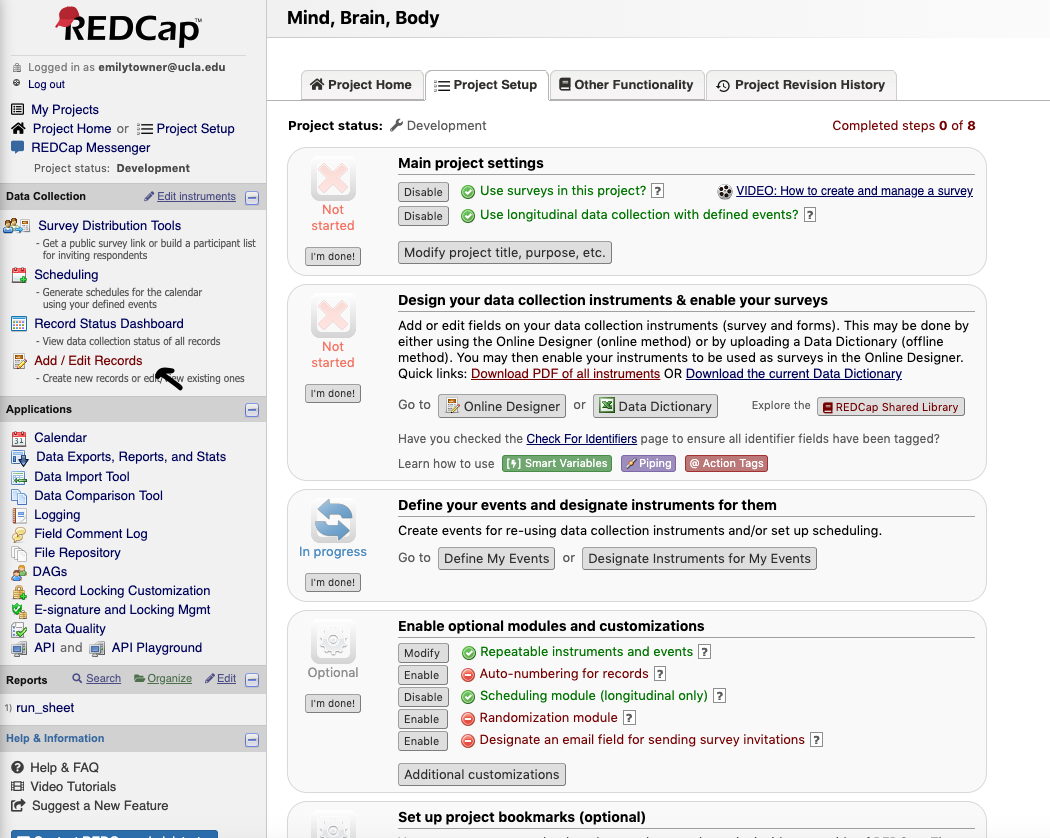
\includegraphics{images/redcap_screening/1.png}
\item
  Click to enter a new Subject ID

  \begin{itemize}
  \tightlist
  \item
    Make sure Arm 1: Recruitment is selected
  \end{itemize}
\item
  Type ``SMBB\#'' (Screener ID) to create a record and hit ``Enter''

  \begin{itemize}
  \tightlist
  \item
    Make sure to link the participants Screener ID and their name on the \textbf{ID Drive ONLY}
  \item
    Before creating a new record, be sure to check the ID Drive to see if the participant already has an existing Screener ID
  \item
    If a record exists, add a new instance of the screen instead of creating a new record
    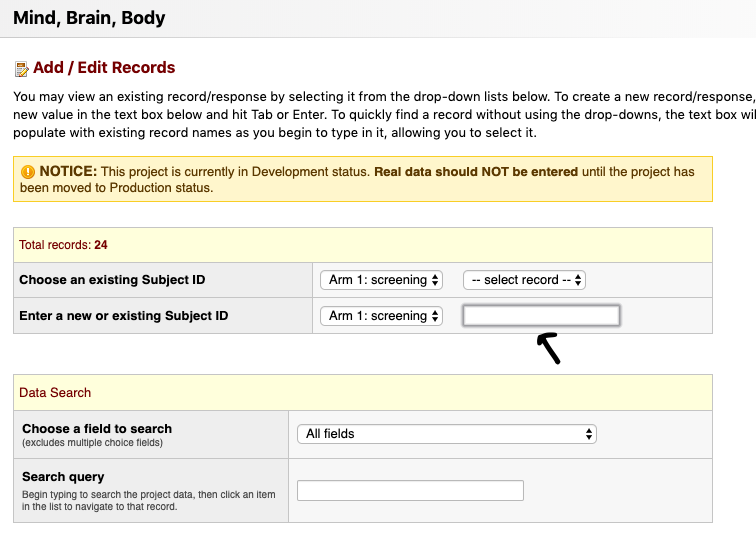
\includegraphics{images/redcap_screening/2.png}
  \end{itemize}
\item
  The screening arm contains two parts

  \begin{itemize}
  \tightlist
  \item
    The screen
  \item
    The wave1\_status

    \begin{itemize}
    \tightlist
    \item
      The wave1\_status is to be updated after the first and each subsequent contact
      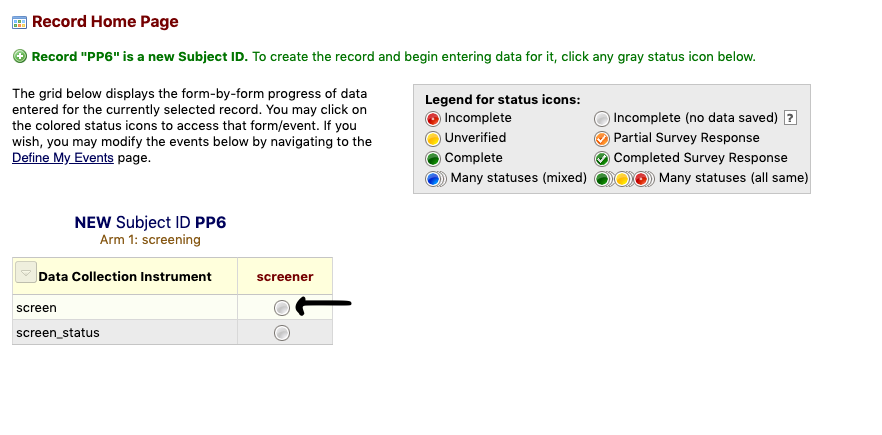
\includegraphics{images/redcap_screening/3.png}
    \end{itemize}
  \end{itemize}
\item
  Click on the radio button in the ``screen'' row to screen the participant
  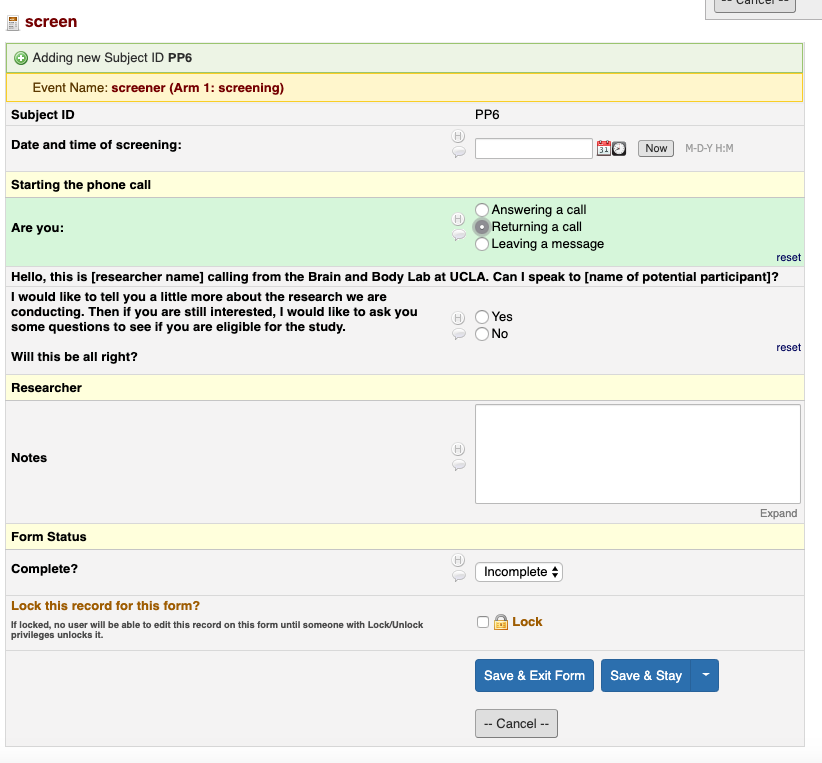
\includegraphics{images/redcap_screening/4.png}
\item
  Click ``Now'' to enter today's date and time
\item
  Select the appropriate choice to start the phone call and follow the skip logic
\item
  Follow the skip logic to the end

  \begin{itemize}
  \tightlist
  \item
    For items without a text field, write the information down in the Recruitment database (This identifying information cannot be on REDCap)
  \end{itemize}
\item
  Once done, select ``Complete'' and ``Save \& Exit Form''

  \begin{itemize}
  \tightlist
  \item
    The screen can be entered multiple times - for instance if there are multiple phone calls or contacts
  \item
    It is important to keep a record of all instances of contact
    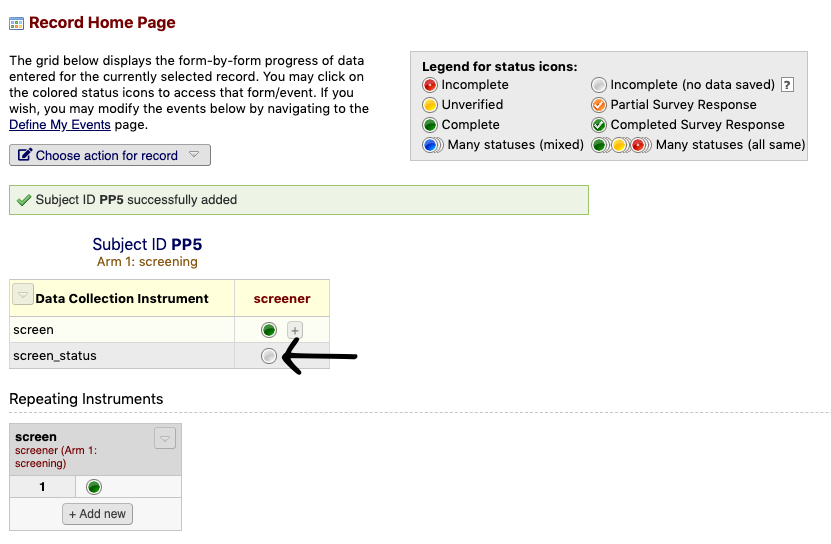
\includegraphics{images/redcap_screening/5.png}
  \end{itemize}
\item
  Click the screen\_status radio button
  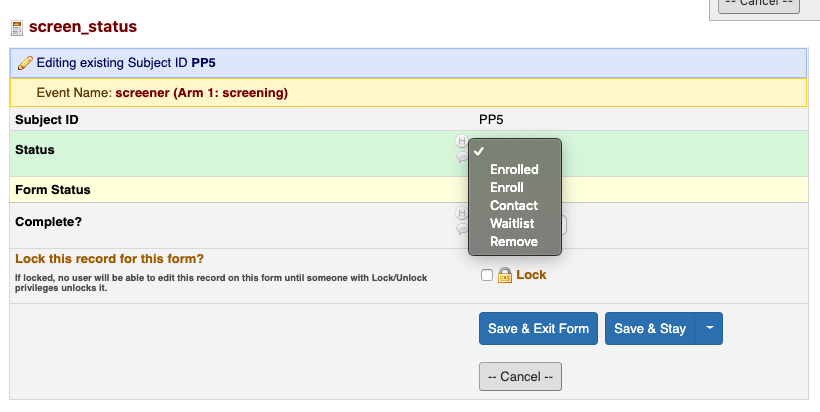
\includegraphics{images/redcap_screening/6.png}
\item
  Select the appropriate option

  \begin{itemize}
  \tightlist
  \item
    Contact - Participant needs to be re-contacted (add Recruitment Database \& ID Drive)
  \item
    Ineligible - Participant not eligible for study
  \item
    To Enroll - Participant to enroll (need to create subject ID, enter subject info, schedule participant, add to Recruitment Database, add to ID Drive)
  \item
    Enrolled - Participant has been enrolled (all above have been completed)
  \item
    To Remove - Participant wants to be removed
  \end{itemize}
\item
  Be sure to update the screen status after each contact

  \begin{itemize}
  \tightlist
  \item
    After 3 contacts (with no response) - review (time of day, contact method, etc.)
  \end{itemize}
\item
  If enrolled, proceed to pre-session checklist in the participant log
\end{enumerate}

\hypertarget{other-screening-information}{%
\subsubsection{Other Screening Information}\label{other-screening-information}}

Accessing Lists

To find out where participants are in the recruitment process, there are several lists.
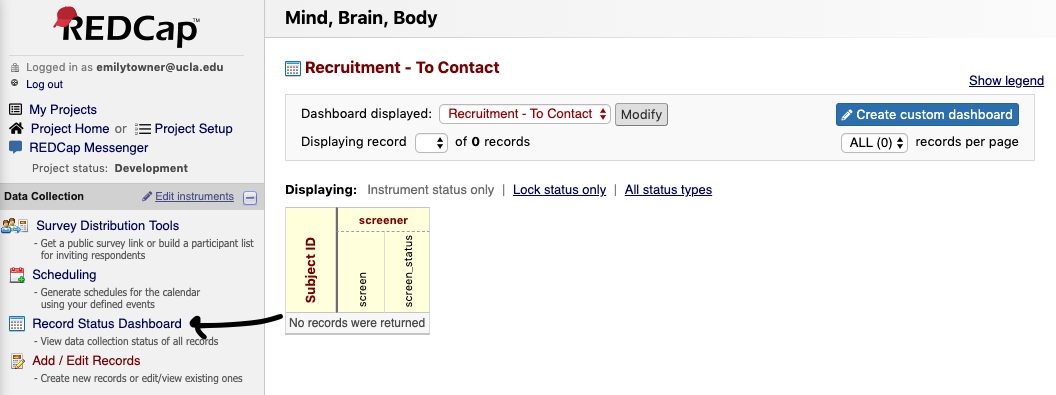
\includegraphics{images/redcap_screening/7.png}
1. Click on ``Record Status Dashboard''
2. Participants who have been enrolled will be listed in the Enrollment - Wave 1 list
3. Participants in the process of recruitment will be listed in one of the 4 Recruitment lists for the appropriate wave
- *These lists are populated based on the individuals ``Screen Status'' so be sure to update after each contact!

List Types

\begin{itemize}
\tightlist
\item
  Contact - List of individuals who need to be contacted or re-contacted (also includes waitlist)
\item
  Ineligible - Participants are ineligible but interested
\item
  To Enroll - Participants who have been screened and are eligible to enroll
\item
  To Remove - Participants who were not interested in being contacted for this or future research
\end{itemize}

\hypertarget{addressing-concerns}{%
\subsubsection{Addressing Concerns}\label{addressing-concerns}}

If a parent has a concern about the study before the session, send the email template:

\begin{itemize}
\tightlist
\item
  {[}MBB - CONCERNS{]}
\end{itemize}

\begin{center}\rule{0.5\linewidth}{0.5pt}\end{center}

\hypertarget{protocol---calendar}{%
\subsection{Protocol - Calendar}\label{protocol---calendar}}

\begin{itemize}
\tightlist
\item
  Lab session events format

  \begin{itemize}
  \tightlist
  \item
    W1 MBBXXX - Lab Session

    \begin{itemize}
    \tightlist
    \item
      MBBXXX - Sex, Age \#, Group
    \item
      Status: Scheduled / Confirmed / Completed
    \item
      Arrival: X AM
    \end{itemize}
  \end{itemize}
\item
  Lab session reminders format

  \begin{itemize}
  \tightlist
  \item
    W1 MBBXXX - Lab Reminder 1 (email)

    \begin{itemize}
    \tightlist
    \item
      Status: Incomplete / Complete
    \end{itemize}
  \item
    W1 MBBXXX - Lab Reminder 2 (Email \& Call)

    \begin{itemize}
    \tightlist
    \item
      Status: Incomplete / Complete
    \end{itemize}
  \end{itemize}
\item
  Home session reminders format

  \begin{itemize}
  \tightlist
  \item
    W1 MBBXXX - Home Reminder 1 (Call)

    \begin{itemize}
    \tightlist
    \item
      Status: Incomplete / Complete
    \end{itemize}
  \item
    W1 MBBXXX - Home Reminder 1 (Email)

    \begin{itemize}
    \tightlist
    \item
      Status: Incomplete / Complete
    \end{itemize}
  \item
    W1 MBBXXX - Home Reminder 2 (Email)

    \begin{itemize}
    \tightlist
    \item
      Status: Incomplete / Complete
    \end{itemize}
  \item
    W1 MBBXXX - Home Reminder 3 (Email)

    \begin{itemize}
    \tightlist
    \item
      Status: Incomplete / Complete
    \end{itemize}
  \end{itemize}
\end{itemize}

\begin{center}\rule{0.5\linewidth}{0.5pt}\end{center}

\hypertarget{protocol---home-kit-assembly}{%
\subsection{Protocol - Home Kit Assembly}\label{protocol---home-kit-assembly}}

Please refer to the diagram below for the complete list of items in a home kit:

\begin{figure}
\centering
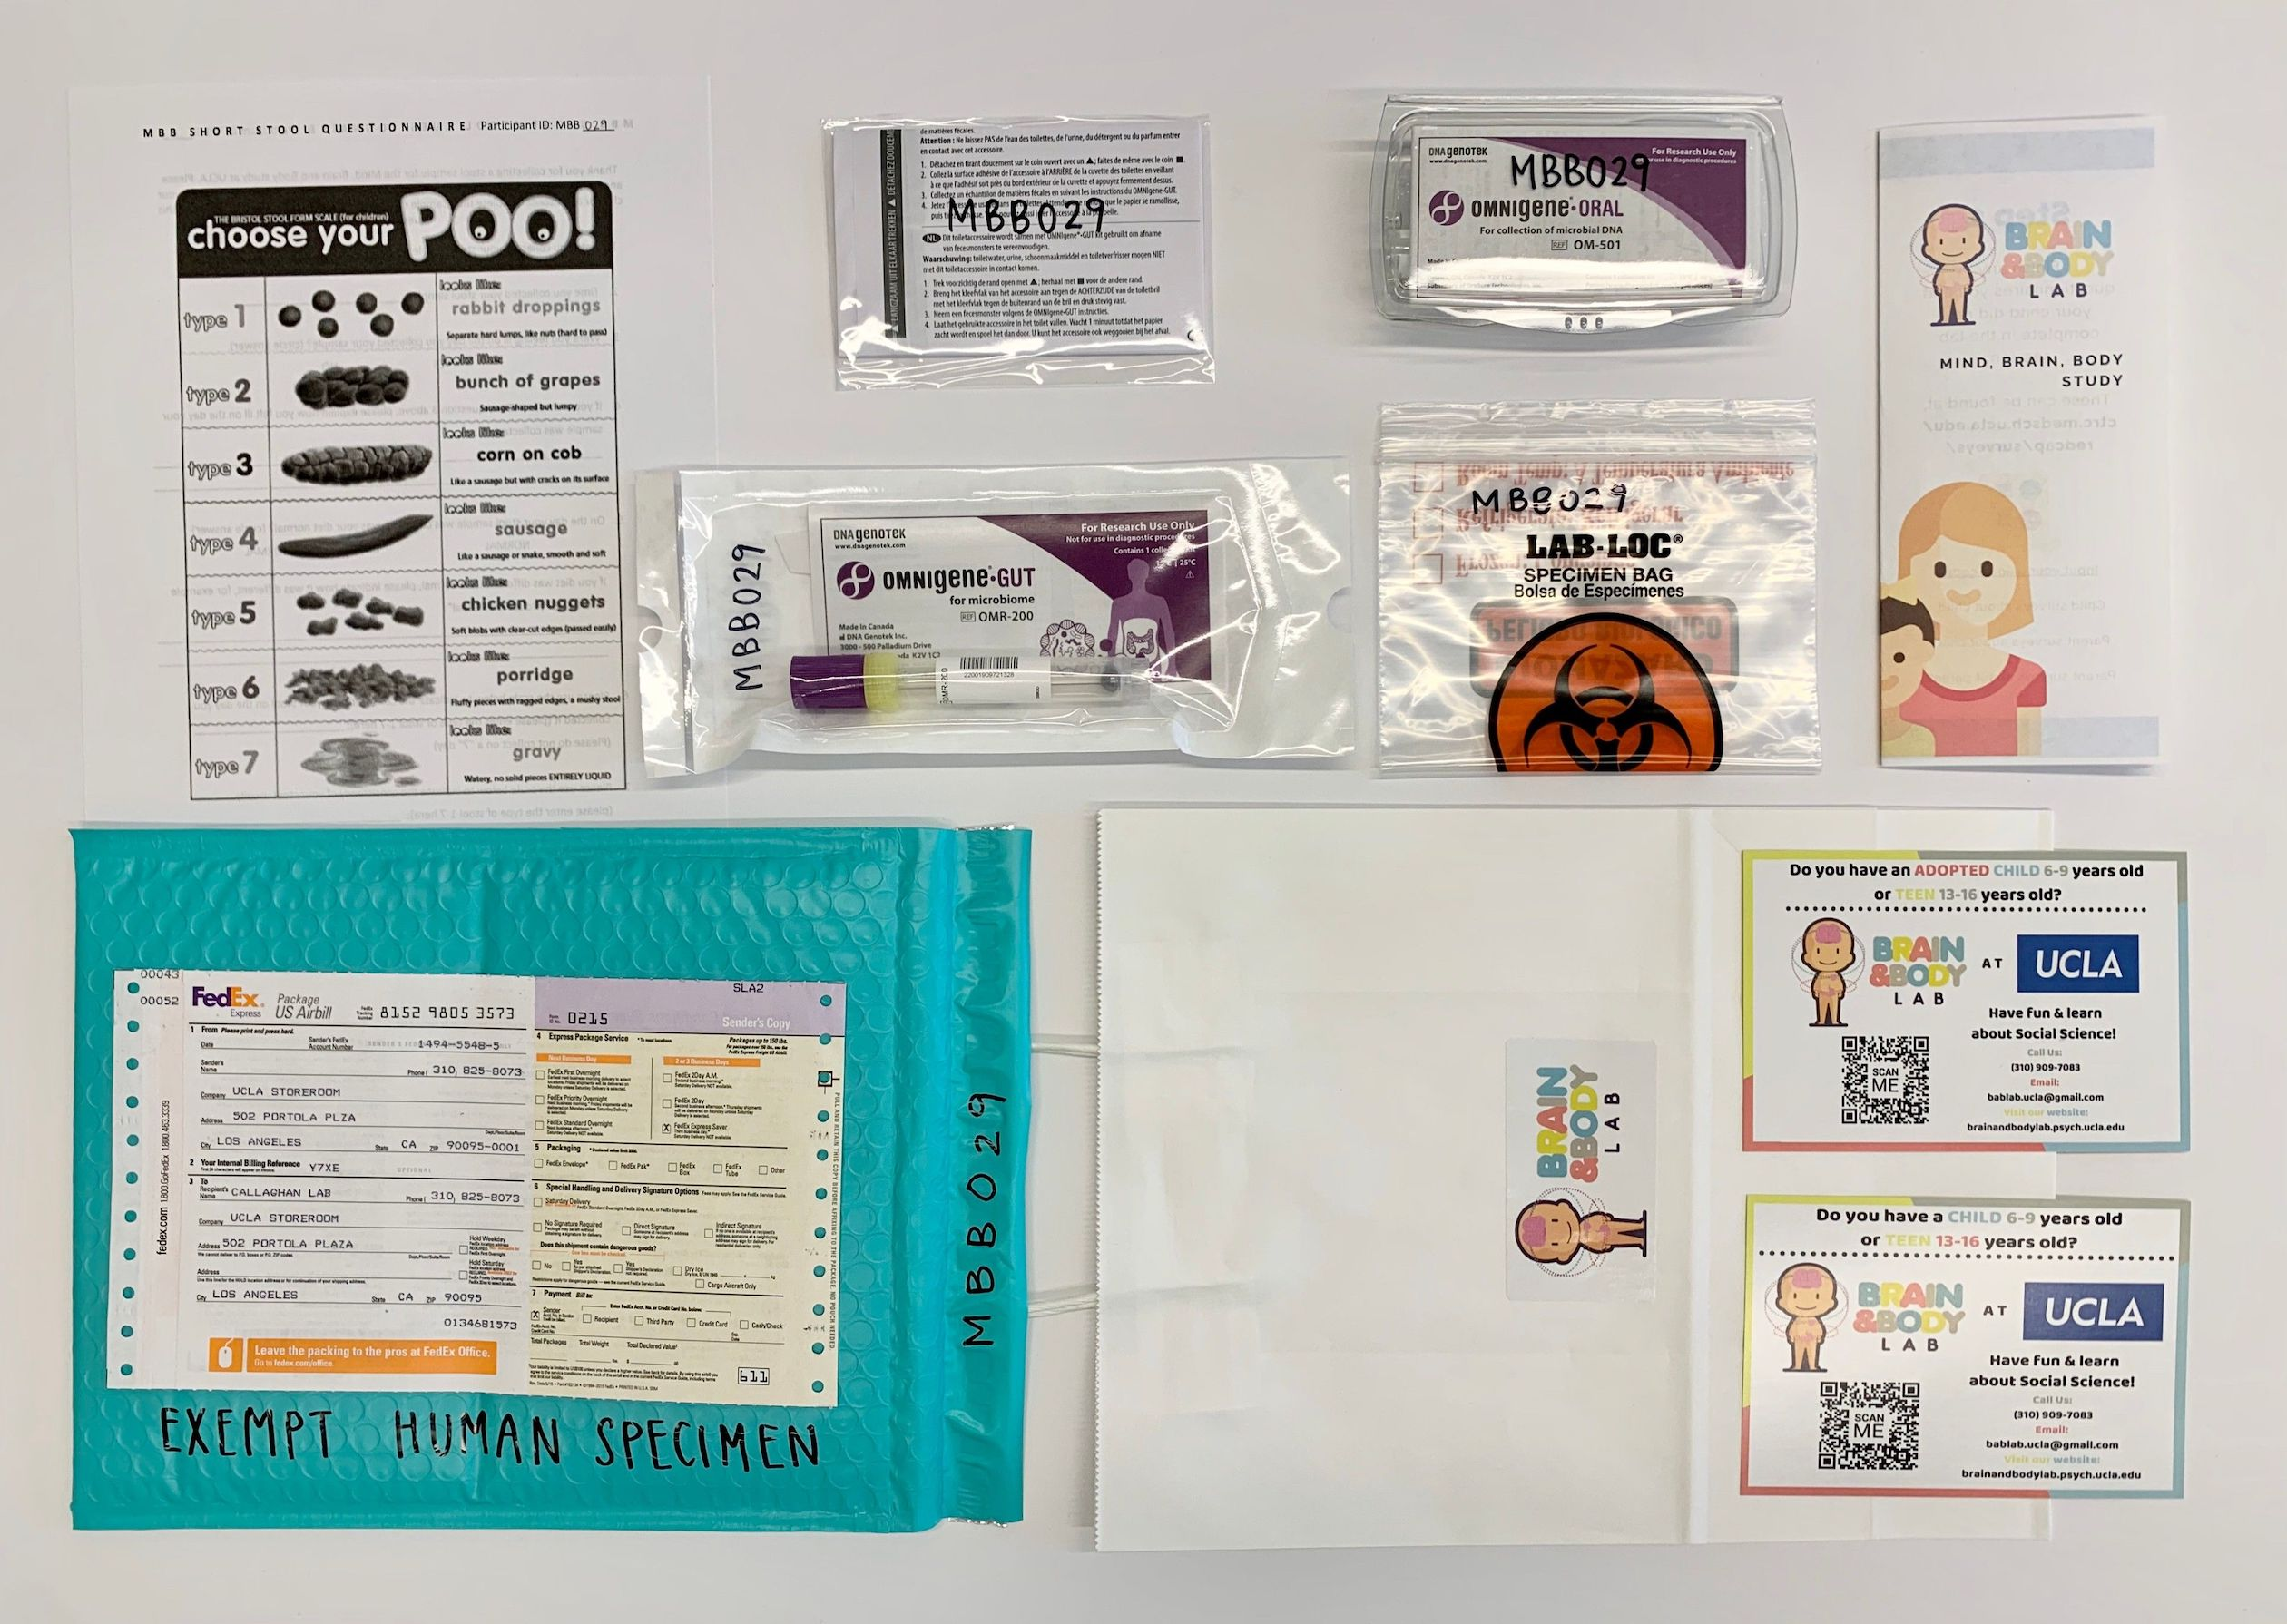
\includegraphics{images/home_kit/1.jpeg}
\caption{}
\end{figure}

\hypertarget{protocols---parent}{%
\section{Protocols - Parent}\label{protocols---parent}}

\hypertarget{protocol---consent-assent}{%
\subsection{Protocol - Consent \& Assent}\label{protocol---consent-assent}}

Once the parent and child/teen come into the lab, seat them in the Rainbow Room on the couch for consenting (parent) and assenting (child aged 7+ or teen).

Make some small talk - Ask the participant how they got here. If they have participated before in research. Offer them a bottle of water. Thank them for coming and for giving up their weekend to help science.

Tell the parent and child that the first thing you are going to do is go over all of the things they will do today, and have them sign the consent and assent forms.

Speak to them and direct them through the whole process.

\hypertarget{things-you-will-do-in-the-lab}{%
\subsubsection{Things you will do in the lab}\label{things-you-will-do-in-the-lab}}

\begin{itemize}
\tightlist
\item
  Stick stickers on you to measure heart rate, sweat, stomach muscles.
\item
  Sit with parent and talk about fun things and hard things (filming).
\item
  Parent stays in room and answers more questions.
\item
  Child goes next door to play computer games (look at pictures, watch movies). Some of the movies and pictures will be a little bit scary, others sad, others boring.
\item
  One of the games involves a loud annoying noise, we will adjust it for you.
\item
  You will also do some other games on paper and pencil - like puzzle and word games
\item
  You will answer some questionnaires
\item
  We will also measure your height, weight, and waist circumference.
\item
  We will take three biological samples:

  \begin{itemize}
  \tightlist
  \item
    Hair - stress hormones
  \item
    Saliva - microbiome
  \item
    Blood - immune - wear goggles
  \end{itemize}
\item
  Do you get sick or dizzy when you see blood or hurt yourself?
\item
  If we need to, can we prick two fingers?
\item
  When you are done with all of that, you will get a big prize, then we will pay you and you will go home.
\item
  You will get \$45 for the work you put in today.
\end{itemize}

\hypertarget{things-you-will-do-at-home}{%
\subsubsection{Things you will do at home}\label{things-you-will-do-at-home}}

Child

\begin{itemize}
\tightlist
\item
  Poop sample - microbiome
\item
  Stool scale
\item
  Memory game - to see what you remember from lab.
\end{itemize}

Parent

\begin{itemize}
\tightlist
\item
  24 hour food recall
\end{itemize}

When you complete the poop sample and the games at home, we will pay you another \$20 in the form of a giftcard.

\hypertarget{things-to-know}{%
\subsubsection{Things to know}\label{things-to-know}}

You are a volunteer, which means that you do not have to do anything, or say anything that makes you uncomfortable. We would like you to try everything you can, and to do your best, but if there are things you absolutely do not want to do, just tell us, that is o.k.

We keep your participation confidential - ID number.

We want you to come in again in the future, so we will ask for some information so we can contact you in the future.

\emph{Sign consent/assent forms including DBS form and Contact Sheet}

\begin{center}\rule{0.5\linewidth}{0.5pt}\end{center}

\hypertarget{protocol---parentchild-observation}{%
\subsection{Protocol - Parent/Child Observation}\label{protocol---parentchild-observation}}

The parent and child will be in the Rainbow Room for 15 minutes. During that time they will be filmed while planning a conflict event, and then again while discussing a pleasant event. The conflict event will always go first, followed by the pleasant event. We did this to ensure that the parents were not thinking of the negative interaction upon answering the questionnaires about their child, which they did immediately after the observation interaction. Participants should complete this activity in English.

\textbf{Step 1}:

Parent and child will be situated on the grey couch in the Rainbow Room. The iPad video camera will be placed about 4 feet away from the dyad, on a tripod stand. The screen of the iPad will be facing away from the parent and child.

\begin{figure}
\centering
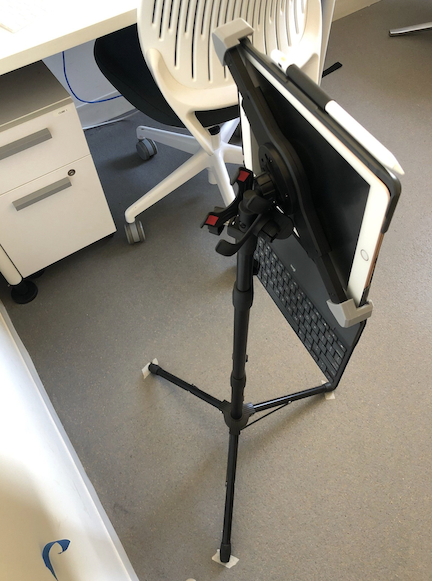
\includegraphics{images/parent:child_obser/2.png}
\caption{}
\end{figure}

\textbf{Step 2}:

The researcher will give the parent and child the Pleasant Events Checklist (PEC) on a piece of paper.

\emph{Researcher: Next we are going to take some film of you while you discuss a source of conflict (or something you disagree on) and try to resolve it. On this piece of paper is a list of things that parents and children sometimes have disagreements about. Please take a moment to read the list and think about some that you would like to discuss together. When I knock on the door, please start discussing the things you have selected from the list and try to resolve the areas of conflict you have chosen from the list. You do not need to tell us what you chose to discuss, and it does not matter if you chose something from the list, or decide to choose something else not included on the list. I will give you five minutes to discuss the event, then I will come back and give you further instructions.}

\textbf{Step 3}:

Researcher press record on the iPad and leave the room. Start timer for 1 minute, then knock on the door and ask the dyad to begin discussing their event. Start timer for 5 minutes. At the end of 5 minutes, again knock on the door and enter the Rainbow Room.

\emph{Researcher: Thank you for taking the time to discuss the source of conflict and try to resolve it. Next we are going to take some film of you while you discuss a pleasant event you could do together. On this piece of paper is a list of events that parents and children sometimes find pleasant to do together. Please take a moment to read the list of events and think about what you would like to plan to do together. When I knock on the door, please start discussing the event you would like to do together and make a plan for how you could do it. You do not need to tell us what you chose to discuss, and it does not matter if you chose something from the list, or decide to choose something else not included on the list. I will give you five minutes to discuss the event, then I will come back and give you further instructions.}

\textbf{Step 4}:

Researcher press record on the iPad and leave the room. Start timer for 1 minute, then knock on the door and ask the dyad to begin discussing their event. Start timer for 5 minutes. At the end of 5 minutes, again knock on the door and enter the Rainbow Room.

\textbf{Step 5}:

Researcher reenter the room, switch the iPad off and move the child/adolescent to their next session.

\begin{center}\rule{0.5\linewidth}{0.5pt}\end{center}

\hypertarget{protocol---ksads}{%
\subsection{Protocol - KSADS}\label{protocol---ksads}}

\hypertarget{audio-recording}{%
\subsubsection{Audio Recording}\label{audio-recording}}

\begin{itemize}
\tightlist
\item
  Make a separate recording for each KSADS administered if there is more than one child in one session.
\end{itemize}

\textbf{Step-by-step guide on how to use recorder:}

\emph{Step 1: Press and hold highlighted Power button to turn recorder.}

\begin{figure}
\centering
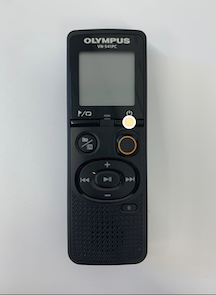
\includegraphics{images/ksads/1.png}
\caption{}
\end{figure}

\emph{Step 2: Press highlighted button until ``TALK'' appears on the screen. Now you are on the ``Talk'' setting.}

\begin{figure}
\centering
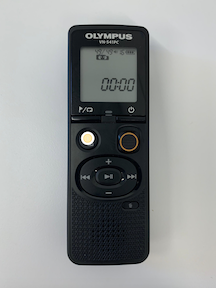
\includegraphics{images/ksads/2.png}
\caption{}
\end{figure}

\emph{Step 3: Push highlighted button up to start recording. Push down to stop recording.}

\begin{figure}
\centering
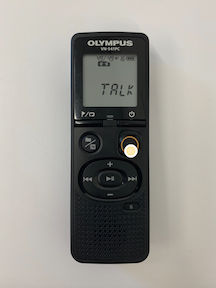
\includegraphics{images/ksads/3.png}
\caption{}
\end{figure}

\hypertarget{using-the-ipad-for-ksads-summary-checklist}{%
\subsubsection{Using the iPad for KSADS Summary Checklist}\label{using-the-ipad-for-ksads-summary-checklist}}

\begin{itemize}
\tightlist
\item
  Before the start of every session, be sure to duplicate and rename all the KSADS documents in Acrobat (25 documents per participant) and rename them (MBBXXX\_KSADS\_suppX\_XXX).

  \begin{itemize}
  \tightlist
  \item
    \emph{Note 1:} This may take a while, especially if there are more than one participant, so be sure to do it ahead of time.
  \item
    \emph{Note 2:} With multiple participants in one session, keep them all on the same iPad as the same iPad will be used to administer all KSADS.
  \end{itemize}
\item
  Follow instructions below on how to duplicate and rename the documents:

  \begin{itemize}
  \item
    Turn on iPad and go to the ``Acrobat'' app.
  \item
    Your screen should look like this. If it does not, tap on ``Files'' at the bottom, and ensure that the Locations is set to ``On This iPad''.

    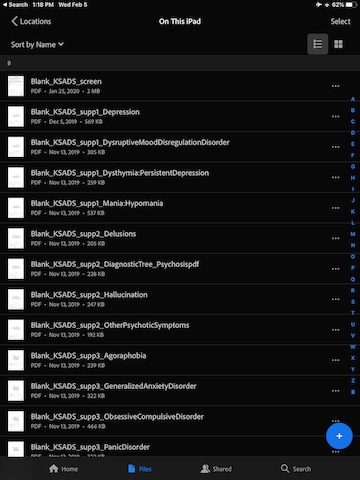
\includegraphics{images/ksads/4.png}
  \item
    For each document, tap the three horizontal dot to the right, and select ``Duplicate''.
    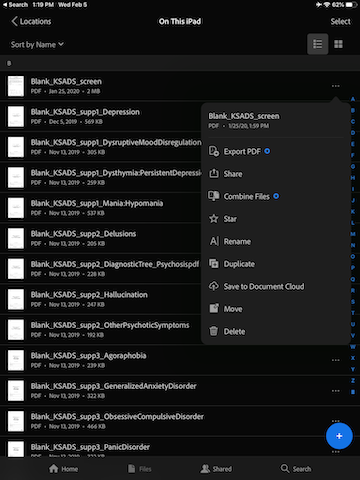
\includegraphics{images/ksads/5.png}
  \item
    The duplicated document should appear right below the original document.
  \item
    Tape the three horizontal dot to the right of the duplicated document, and select ``Rename''.
    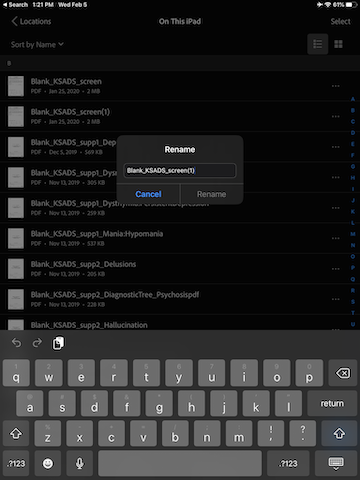
\includegraphics{images/ksads/6.png}
  \item
    Replace the word ``Blank'' with the participant ID, and remove the ``(1) at the end of the name. For example, if the participant ID is MBB001, the name of the duplicated document should be: MBB001\_KSADS\_screen
  \item
    Do the same for all 25 documents (Duplicate, Rename).
  \end{itemize}
\end{itemize}

\begin{center}\rule{0.5\linewidth}{0.5pt}\end{center}

\hypertarget{protocol---questionnaires}{%
\subsection{Protocol - Questionnaires}\label{protocol---questionnaires}}

\hypertarget{parent-proxy}{%
\subsubsection{Parent Proxy}\label{parent-proxy}}

Parents will complete REDCap questionnaires for each child.

\hypertarget{parent-self}{%
\subsubsection{Parent Self}\label{parent-self}}

Parents will complete REDCap questionnaires about themselves only once (under eldest child's {[}lower number{]} ID)

\begin{center}\rule{0.5\linewidth}{0.5pt}\end{center}

\hypertarget{protocol---home-kit}{%
\subsection{Protocol - Home Kit}\label{protocol---home-kit}}

Explain to the parent what is included in the home kit / home session and how to collect the stool sample.

\begin{center}\rule{0.5\linewidth}{0.5pt}\end{center}

\hypertarget{protocols---childteen}{%
\section{Protocols - Child/Teen}\label{protocols---childteen}}

\begin{center}\rule{0.5\linewidth}{0.5pt}\end{center}

\hypertarget{protocol---biopac-electrode-hookup}{%
\subsection{Protocol - BioPac Electrode Hookup}\label{protocol---biopac-electrode-hookup}}

\hypertarget{electrode-placementpreparation}{%
\subsubsection{Electrode Placement/Preparation}\label{electrode-placementpreparation}}

\begin{itemize}
\tightlist
\item
  Wheel the cart into the Rainbow Room
\item
  Prep 2 electrodes with Gel 101. Stick to the participant's ring and middle fingers on their non-dominant hand (we want to keep the pointer finger free so they can use it for tasks)
\item
  Wrap medical tape around these to secure them, but ensure that the metal poles are still accessible
\item
  Look at the skeleton diagram and use the EL-PREP Gel to abrade the skin around the remaining electrode sites (below the collarbones, below the sternum, on the left lower ribs, and in the remaining two positions on the stomach and left ribs)
\item
  Clean the remaining EL-PREP off with a tissue or baby wipe
\item
  Prep 8 electrodes with Gel 100. Stick to the locations indicated on the skeleton diagram
\item
  Let all electrodes sit for the duration of the parent/child observation
\end{itemize}

\begin{figure}
\centering
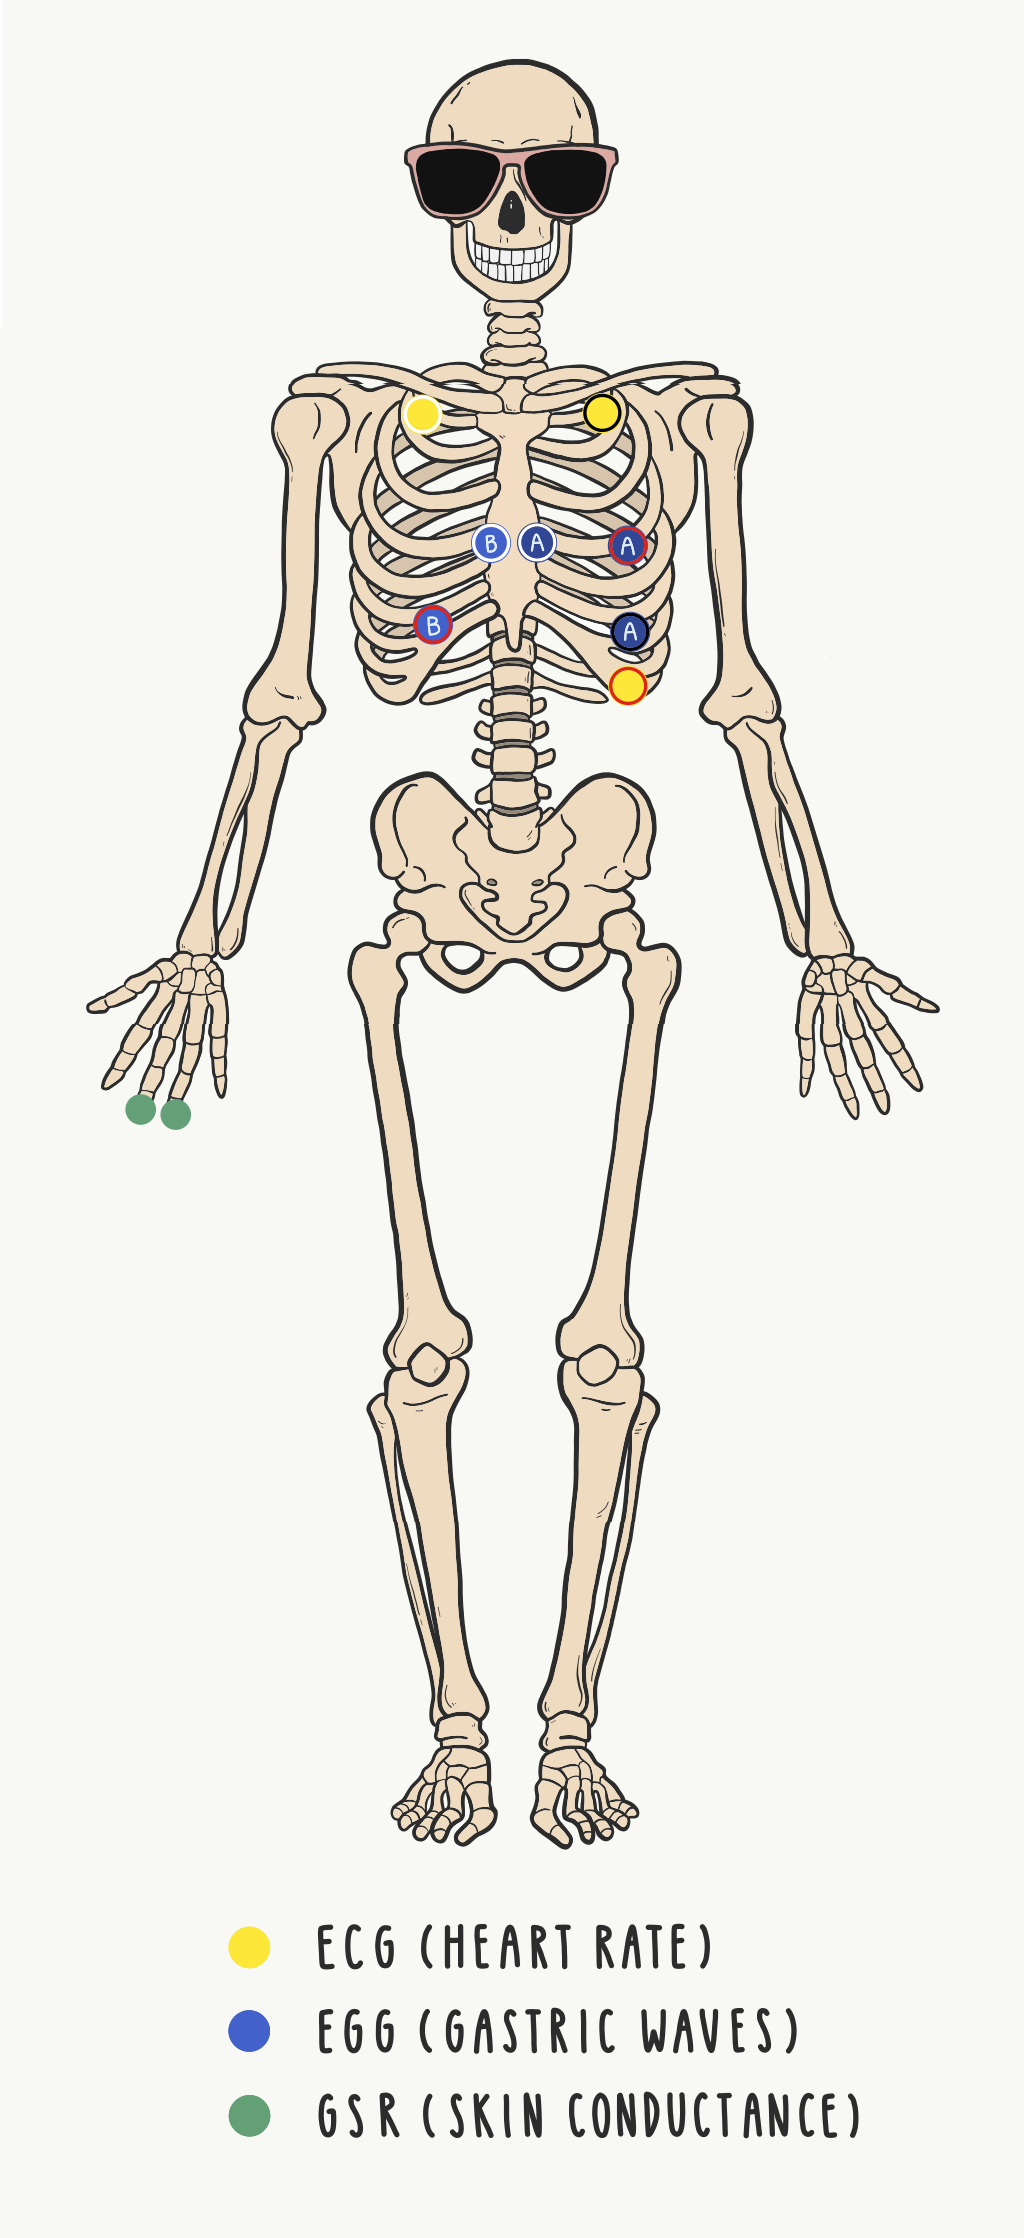
\includegraphics{images/physiology/1.png}
\caption{}
\end{figure}

\hypertarget{gsr}{%
\subsubsection{GSR}\label{gsr}}

\begin{itemize}
\tightlist
\item
  Put on gloves
\item
  Ensure that the finger electrodes are properly adhered and have had time to rest
\item
  Make sure the lead wire module is connected to the transmitter (PPGED, green sticker) in the ``EDA'' channel
\item
  Take the transmitter and secure it around the participant's wrist as shown below
\item
  Hook up the lead wires so that the black wire connects to the middle finger and the red wire connects to the ring finger
\item
  Ask the participant to wear a glove over the whole setup to secure it throughout the tasks
\item
  To check if the GSR is working properly, ask the participant to briefly hold his/her breath - you should see a rise in the signal on the graph
\end{itemize}

\hypertarget{ecg}{%
\subsubsection{ECG}\label{ecg}}

\begin{itemize}
\tightlist
\item
  Ensure that the chest electrodes are properly adhered and have had time to rest.
\item
  Make sure the lead wire module is connected to the transmitter (RSPEC-R, yellow sticker) in the ECG channel.
\item
  Take the transmitter and secure it around the participant's stomach as shown below.
\item
  Hook up the lead wires so that the white lead connects to the Right Collarbone electrode, the black lead connects to the Left Collarbone electrode, and the red lead connects to the lowest Left Rib electrode.
\end{itemize}

\hypertarget{egg}{%
\subsubsection{EGG}\label{egg}}

\begin{itemize}
\tightlist
\item
  Ensure that the chest electrodes are properly adhered and have had time to rest.
\item
  Make sure the lead wires are connected to the transmitter (EGG2-R, blue sticker). The lead module labelled ``A'' (3 short leads) should be in the EGG A channel, while the lead module labelled ``B'' (2 long leads) should be in the EGG B channel.
\item
  Take the transmitter and secure it around the participant's stomach as show below.
\item
  Hook up the lead wires so that the ``A'' and ``B'' channel white leads connect to the sternum electrodes (which goes to which does not matter), the ``A'' and ``B'' channel red leads connects to the upper left rib electrode and stomach electrode, and the ``B'' channel black lead connects to the remaining lower left rib electrode.
\end{itemize}

\hypertarget{acqknowledge}{%
\subsubsection{AcqKnowledge}\label{acqknowledge}}

\begin{itemize}
\tightlist
\item
  Turn off the wifi on the Mac Mini and turn on the BioPac/transmitters
\item
  Open AcqKnowledge
\item
  Choose the graph template file
\item
  Once it loads, make sure all of the transmitters are connected
\item
  Press run and click through all of the dialog boxes that are generated
\end{itemize}

\begin{center}\rule{0.5\linewidth}{0.5pt}\end{center}

\hypertarget{protocol---memory-intrusionmovie-watching}{%
\subsection{Protocol - Memory Intrusion/Movie Watching}\label{protocol---memory-intrusionmovie-watching}}

\begin{itemize}
\item
  There are 4 counterbalanced versions of this task:

  \begin{itemize}
  \tightlist
  \item
    DRM\_A\_incongruent\_first.psyexp
  \item
    DRM\_A\_congruent\_first.psyexp
  \item
    DRM\_B\_congruent\_first.psyexp
  \item
    DRM\_B\_incongruent\_first.psyexp
  \end{itemize}
\item
  Choose the counterbalanced version that is correct for the participant
\item
  First open the task, add the participant ID number and press start
\item
  Read the instructions to the participant:

  \emph{Welcome to the movie game. First you will watch some movies. Then you will hear a list of words. Try to remember the words on the list.}
\item
  Press the space bar to progress to the next screen and read the instructions:

  \emph{Get ready, to watch the movie. Turn to the laptop to watch.}
\item
  Open up the first movie for the participant. It will depend on the counterbalancing condition what movie goes first.
\item
  For the two files that start with ``DRM\_A'':

  \begin{itemize}
  \tightlist
  \item
    DRM\_A\_congruent\_first.psyexp
  \item
    DRM\_A\_incongruent\_first.psyexp
  \end{itemize}
\end{itemize}

\textbf{The order will be: Sad --\textgreater{} Neutral --\textgreater{} Scary}

\begin{itemize}
\tightlist
\item
  For the two files that start with ``DRM\_B'':

  \begin{itemize}
  \tightlist
  \item
    DRM\_B\_congruent\_first.psyexp
  \item
    DRM\_B\_incongruent\_first.psyexp
  \end{itemize}
\end{itemize}

\textbf{The order will be: Scary --\textgreater{} Neutral --\textgreater{} Sad}

\begin{itemize}
\item
  Simultaneously press play on the movie on the laptop while also pressing the spacebar on the psychopy task. This will start the physiology and the movie at about the same time. While the movie is playing there will be a box of popcorn on the computer screen.
\item
  When the movie is done, press spacebar on the psychopy computer to progress to the next screen. Read the instructions for the participant:
\item
  Click on the face that shows how you feel after watching the movies.
\item
  Participants can use a mouse to click on the face that matches the way they feel after watching the movie. The faces range in valence (negative to positive) across the X axis, and arousal (low to high) up the Y axis.
\item
  After the participant has selected a face, you will be taken to the next screen where you can read the instructions for the participants:

  \emph{Listen to the list of words and try to remember all of them.}
\item
  When the participant indicates that they have understood the instructions, press the spacebar and progress to the next screen. Make sure that the computer volume is up and the participant can hear the words being pronounced on the computer screen. After the participant hears all the words the distractor task will start.
\item
  Read the distractor task instructions to the participant:

  \emph{Count backwards from the number 25 out loud for the researcher.}
\end{itemize}

\textbf{Note: Whether the participant completes the distractor task correctly or not doesn't matter. The only purpose of the distractor task is to distract the participant for a brief period of time. Listen while they count backwards. If they can't count backwards, ask them to count forwards.}

\begin{itemize}
\item
  When the participant is finished counting backwards from 25, or after approximately 30s has passed (whatever comes first), progress to the next screen by pressing the spacebar.
\item
  Read the instructions out loud to the participant:

  \emph{Recall 1. Please tell the researcher all the words that you can remember from the list.}
\item
  Before the participant starts to tell you what they remember, start a new voice recording and then tell them to start while you record what they say (on the talk setting). Also write what they say on a piece of paper. Make sure to note that this is `Recall 1' (as there is a second recall later on). When the participant has told you all the words they can remember, or after 60s, progress to the next screen (instructions for the next word list).
\item
  Make one recording for all of the memory intrusion task
\item
  Read the instructions aloud for the participant.

  \emph{Now you will hear another word list. Get ready!}
\item
  Press the spacebar to hear the word list. After the word list, move to the distractor task (counting backwards from 25). After the distractor task, move to the second recall task and record the participant like the first. When the second recall task is complete, a new loop will begin. Read the instructions to the participant then start the next movie (which will always be neutral). Repeat everything again for the final loop after they watch the final movie, which will either be sad or scary.
\end{itemize}

\begin{center}\rule{0.5\linewidth}{0.5pt}\end{center}

\hypertarget{protocol---halloween}{%
\subsection{Protocol - Halloween}\label{protocol---halloween}}

\begin{itemize}
\item
  Check master counterbalance sheet and fill out the participant's ID \# in the group which you assigned them.
\item
  Seat the participant at the computer desk in the Bear's Den. Close the door to ensure privacy and freedom from distractions.
\item
  Set up the task:

  \begin{itemize}
  \item
    \begin{enumerate}
    \def\labelenumi{\alph{enumi}.}
    \tightlist
    \item
      Navigate through the Finder to get to the task following this path:
      Dropbox/BAB/Studies/Mind\_Brain\_Body/Tasks/Wave1/04\_halloween\_pilot
      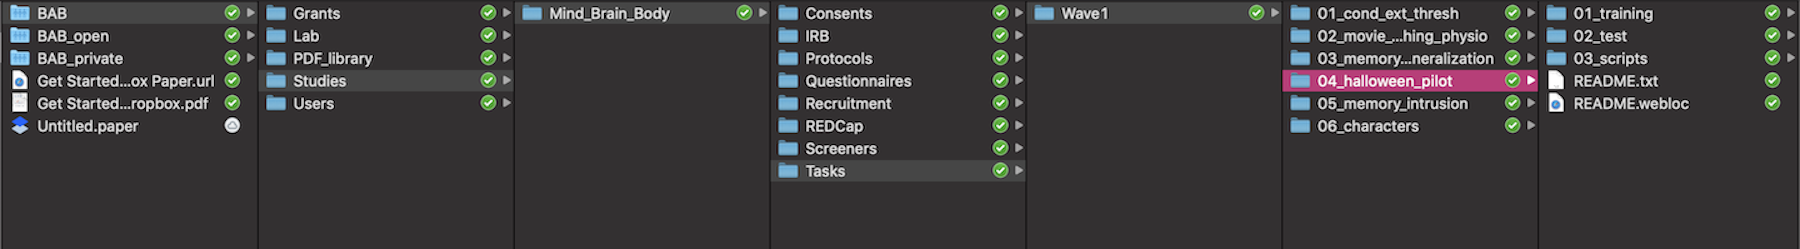
\includegraphics{images/halloween/1.png}
    \end{enumerate}
  \item
    \begin{enumerate}
    \def\labelenumi{\alph{enumi}.}
    \setcounter{enumi}{1}
    \item
      Start by going into the folder titled ``01\_training'' and selecting ``Halloween\_training\_day1.psyexp'' if the participant is in the ``day first'' group or ``Halloween\_training\_night1.psyexp'' if the participant is in the ``night first'' group.

      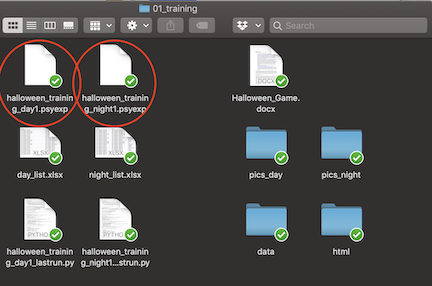
\includegraphics{images/halloween/2.png}
    \end{enumerate}
  \end{itemize}
\item
  When the task pulls up and the participant is situated and ready, select the run button indicated below:

  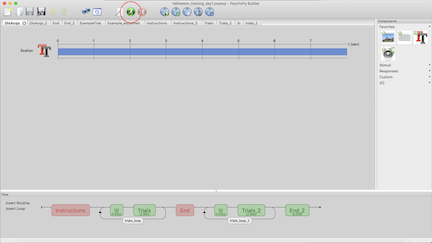
\includegraphics{images/halloween/3.png}
\item
  When prompted, fill in the participant's ID \# in the ``participant'' field:
  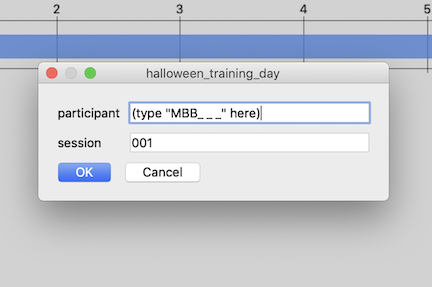
\includegraphics{images/halloween/4.png}
\item
  Guide the participant through the instructional slides by pressing the space bar every time {[}s{]} shows up on the screen. Make sure to remind the participant to read all of the instructions carefully.
\item
  Once the training task starts, sit quietly and do not disturb the participant. It is important for them to pay their undivided attention to the images on screen during the training.
\item
  When the break slide appears, ask them to let you know when they are ready to continue. Press the space bar to proceed on to the next set of images.
\item
  Once the task is complete, you can exit out by pressing any key and then closing the the PsychoPy file.
\item
  Prompt the testing phase of the exercise by saying something along the lines of:
  \emph{``And now we want to see how much of your trick-or-treating adventure you remember.''}
\item
  Go into the ``02\_test'' file and select the ``Halloween\_day1.psyexp'' file if the participant is in the ``day first'' group or ``Halloween\_night1.psyexp'' if the participant is in the ``night first'' group.
  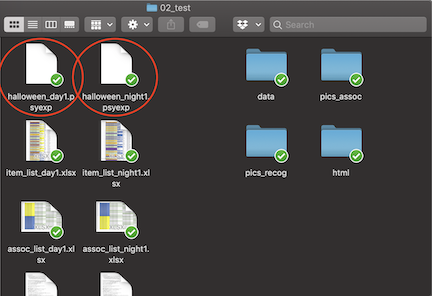
\includegraphics{images/halloween/5.png}
\item
  When the task pulls up and the participant is situated and ready, select the run button indicated below:

  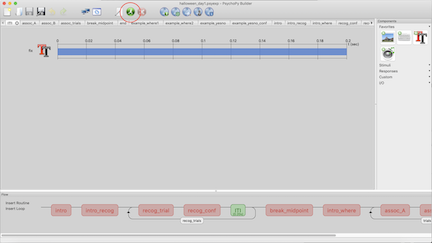
\includegraphics{images/halloween/6.png}
\item
  Guide the participant through the instructional slides by pressing the space bar every time {[}s{]} shows up on the screen. Make sure to remind the participant to read all of the instructions carefully. Remind them that they need to click the words for the answer they want to provide.
\item
  When the break slide appears, ask them to let you know when they are ready to continue. Press the space bar to proceed on to the next tests.
\item
  Guide the participant through the instructional slides by pressing the space bar every time {[}s{]} shows up on the screen. Make sure to remind the participant to read all of the instructions carefully. Remind them that they need to click the item for the answer they want to provide, and then click which quadrant of the scene image they want to pick.
\item
  Once the task is complete, you can exit out by pressing any key and then closing the the PsychoPy file.
\item
  Data is saved automatically in the data folder. You do not need to save anything before exiting out of the psychopy folder
\end{itemize}

\emph{Troubleshooting:}

If the task exits due to an error, take a screenshot of the error screen and message Emily, Kristen, or Bridget for assistance. Move onto the next task in the meantime.

\begin{center}\rule{0.5\linewidth}{0.5pt}\end{center}

\hypertarget{protocol---disccondext}{%
\subsection{Protocol - Disc/Cond/Ext}\label{protocol---disccondext}}

\hypertarget{discrimination}{%
\subsubsection{Discrimination}\label{discrimination}}

\begin{itemize}
\tightlist
\item
  Click into the discrimination folder
\item
  Right click on either discrimination\_horiz.py or discrimination\_vert.py (depending on counterbalancing) and open in PsychoPy

  \begin{itemize}
  \tightlist
  \item
    This task was not created in Builder view, so does not have a .psyexp file.
  \end{itemize}
\item
  Click the green running man and enter the Participant ID

  \begin{itemize}
  \tightlist
  \item
    Make sure to enter the correct run number
  \item
    Discrimination will be repeated 3 times (run 1, run 2, and run 3)
  \end{itemize}
\item
  Move the keyboard over so that the you, the researcher, can control it

  \begin{itemize}
  \tightlist
  \item
    You will press the buttons for the participant in this task (it is difficult to do and pay attention to on one's own)
  \end{itemize}
\item
  Read the instructions for the participant
\item
  Ask the participant to tell you which line was more tilted, the first or second and press the corresponding button for them
\end{itemize}

\hypertarget{conditioning}{%
\subsubsection{Conditioning}\label{conditioning}}

\begin{itemize}
\tightlist
\item
  Click into the conditioning folder

  \begin{itemize}
  \tightlist
  \item
    Test the sound file on the laptop - screech.ogg
  \item
    Set so that the sound is loud and uncomfortable, but not hurting
  \item
    Record the volume setting on the session checklist
  \end{itemize}
\item
  Open the .psyexp file for the appropriate counterbalance by right clicking and opening in PsychoPy
\item
  Click the green running man icon and enter the Participant ID
\end{itemize}

\hypertarget{extinction}{%
\subsubsection{Extinction}\label{extinction}}

\begin{itemize}
\tightlist
\item
  Click into the extinction folder
\item
  Open the .psyexp file
\item
  Click the green running man icon and enter the Participant ID
\end{itemize}

\begin{center}\rule{0.5\linewidth}{0.5pt}\end{center}

\hypertarget{protocol---height}{%
\subsection{Protocol - Height}\label{protocol---height}}

\begin{itemize}
\tightlist
\item
  Place participant directly against wall/frame
\item
  Advise participant to stand up straight
\item
  Make sure heels of participant are up against the wall/frame
\item
  Use a flat object (booklet, ruler, sheet of paper, etc.) to accurately measure height in centimeters
\item
  Record height on Lab Session Checklist
\end{itemize}

\begin{center}\rule{0.5\linewidth}{0.5pt}\end{center}

\hypertarget{protocol---hair-sample}{%
\subsection{Protocol - Hair Sample}\label{protocol---hair-sample}}

\hypertarget{training-video}{%
\subsubsection{Training video}\label{training-video}}

\hypertarget{set-up-hair-sample-station}{%
\subsubsection{Set Up Hair Sample Station}\label{set-up-hair-sample-station}}

\begin{itemize}
\tightlist
\item
  Ensure the hair-sample station is set up accordingly:

  \begin{itemize}
  \tightlist
  \item
    1 sheet of aluminum foil
  \item
    1 small ziplock bag with participant ID
  \item
    1 salon grade scissor
  \item
    1 wide and narrow tooth parting comb
  \item
    1 alcohol swab
  \item
    Painter-tape
  \item
    1 permanent marker
  \item
    1 pair of gloves
  \item
    2 alligator curl clips
  \item
    1 hair claw clip (for long hair)
  \item
    Sample hair amount taken from wig
  \end{itemize}
\end{itemize}

\hypertarget{prior-to-getting-hair-sample}{%
\subsubsection{Prior to Getting Hair Sample}\label{prior-to-getting-hair-sample}}

\begin{itemize}
\tightlist
\item
  With the parent present in the room, explain to both the child and parent that we will be collecting 30-50 strands of hair. The amount of hair to be collected is less hair than is lost in normal everyday-brushing from the back of the head.
\item
  Inform them how the site for the sampling is hidden by the surrounding hair, therefore not visible after collection.
\item
  Explain how the sample is used to measure a hormone called cortisol that is present in the hair.
\item
  Show the hair sample taken from the wig to illustrate the amount of hair that will be collected (30-50 strands).
\item
  Complete the \href{https://app.box.com/file/630323877918}{Hair-Care Practice Questionnaire}.
\end{itemize}

\hypertarget{hair-sample-prep}{%
\subsubsection{Hair Sample Prep}\label{hair-sample-prep}}

\begin{itemize}
\tightlist
\item
  Ask the parent to be present in the room when we collect the child's hair sample.
\item
  Put on a pair of gloves.
\item
  Wipe down the hair scissor/comb/clips with an alcohol swab.
\end{itemize}

\hypertarget{hair-length}{%
\subsubsection{Hair Length}\label{hair-length}}

\begin{itemize}
\tightlist
\item
  For short hair (less than 3cm), follow the Short-Hair Protocol below.
\item
  For medium-length hair (3-6cm), follow the Medium-Hair Protocol below.
\item
  For long hair (more than 6cm), follow the Long-Hair Protocol below.
\item
  Ideally, all hair sample should be at least 3cm long. If the hair is less than 1cm long, the sample cannot be used.
\end{itemize}

\textbf{Short-Hair Protocol (1-3cm)}

\begin{itemize}
\tightlist
\item
  Take the comb and part the hair horizontally between the tips of the ears.
\item
  After parting, ask the participant to hold the parted hair close to the scalp.
\item
  Hold the loose hair tightly with index finger and thumb, and cut the hair along the part.
\item
  Place loose hairs in foil and fold it securely. Do not tape the hair to the foil.
\item
  Fold the foil without bending the hair, and ensure that the hair does not fall out of the foil.
\item
  Label the root-end on the aluminum foil and place it in the ziplock bag.
\item
  Label the ziplock bag with the participant's ID.
\item
  Store the sample in a dry area at room temperature (in the plastic folder under the participant ID in cabinet 1).
\end{itemize}

\textbf{Medium-Hair Protocol (3-6cm)}

\begin{itemize}
\tightlist
\item
  Take the comb and part the hair horizontally between the tips of the ears.
\item
  Take a clip to clip away the hair from the top of the parting.
\item
  Place another clip at the bottom to expose a 5x10cm rectangle of loose hair between the two clips.
\item
  Ask if the child prefers the wide or narrow tooth comb to comb through the loose hair.
\item
  Ask if it is ok to discard any loose hair from the comb.
\item
  Grasp approx. 30-50 strands of hair to the right of the rectangle.
\item
  Gently pull and twist the hair away from the scalp in a rolling motion between the fingers.
\item
  Collect the sample as close to scalp as possible, but be careful to not cut the scalp.
\item
  Attach the hair to the center of the aluminum foil by taping with painter's tape - do not cover the root end.
\item
  Label the root end on the tape.
\item
  Fold the foil without bending the hair, and ensure that the hair does not fall out of the foil.
\item
  Label the root-end on the aluminum foil and place it in the ziplock bag.
\item
  Label the ziplock bag with the participant's ID.
\item
  Store the sample in a dry area at room temperature (in the plastic folder under the participant ID in cabinet 1).
\end{itemize}

\textbf{Long-Hair Protocol (\textgreater{}6cm)}

\begin{itemize}
\tightlist
\item
  Part the hair left to right at the posterior vertex.
\item
  Clip away any extra hair, then create a twist of hair and hold tightly with index finger and thumb.
\item
  Make a clean cut as close to scalp as possible.
\item
  If the hair is thin, cut 2-3 small areas (1cm apart) across the posterior vertex to conceal the site of the cut.
\item
  Attach the hair to the center of the aluminum foil by taping with painter's tape - do not cover the root end.
\item
  Label the root end on the tape.
\item
  Fold the foil without bending the hair, and ensure that the hair does not fall out of the foil.
\item
  Label the root-end on the aluminum foil and place it in the ziplock bag.
\item
  Label the ziplock bag with the participant's ID.
\item
  Store the sample in a dry area at room temperature (in the plastic folder under the participant ID in cabinet 1).
\end{itemize}

\begin{center}\rule{0.5\linewidth}{0.5pt}\end{center}

\hypertarget{protocol---weight}{%
\subsection{Protocol - Weight}\label{protocol---weight}}

\begin{itemize}
\tightlist
\item
  Instruct participant to step on weight scale
\item
  Measure weight (in kg)
\item
  Record weight on Lab Session Checklist
\end{itemize}

\begin{center}\rule{0.5\linewidth}{0.5pt}\end{center}

\hypertarget{protocol---saliva-sample}{%
\subsection{Protocol - Saliva Sample}\label{protocol---saliva-sample}}

Sample Storage:

\begin{itemize}
\tightlist
\item
  Screw lids on very tight (to prevent evaporation)
\item
  Log the location (grid) on the sample storage log
\end{itemize}

\begin{center}\rule{0.5\linewidth}{0.5pt}\end{center}

\hypertarget{protocol---memory-generalization}{%
\subsection{Protocol - Memory Generalization}\label{protocol---memory-generalization}}

\hypertarget{training}{%
\subsubsection{Training}\label{training}}

\begin{itemize}
\tightlist
\item
  There are two versions of this task (They differ in the pictures that are used for training):

  \begin{itemize}
  \tightlist
  \item
    memory\_generalization\_beta.psyexp
  \item
    memory\_generalization\_beta\_B.psyexp
  \end{itemize}
\item
  Run the task on PsychoPy.
\item
  Read the instructions out loud to the participant.
\item
  When you see ``{[}s{]}'' it means that you can progress to the next screen.
\item
  There will be 60 photographs the participant has to see. They are presented in random order.
\item
  There are 10 red triangles. The participant is asked to press a button when they see the red triangles so that we can later on gauge their attention in the task.
\item
  After the 60 photographs are shown, the participant is asked to recall all of the photos they just saw. Press record on the recorder (on talk setting). Make one recording for the whole memory generalization task.
\item
  They will go through this photo viewing and recall phase another 2 times.
\item
  When the task is complete, save the PsychoPy output file, as well as the recorded responses to the participant folder on the Dropbox.
\end{itemize}

\hypertarget{test}{%
\subsubsection{Test}\label{test}}

\begin{itemize}
\tightlist
\item
  Immediately after the memory generalization training, administer the memory generalization test.
\item
  There is only one version of the memory generalization test: memory\_test.psyexp
\item
  Read the instructions to the participant, emphasizing that we only want them to respond YES if the picture is EXACTLY the same as the one they just saw in the training task.
\item
  If the participant responds ``Yes'' or ``No'' they will progress to a confidence rating screen, asking them how sure they are in their response.
\item
  If the participant responds ``I Don't Know'' they will skip the confidence rating screen.
\item
  When the task is complete, save the participants data output from PsychoPy into their participant folder on the server.
\end{itemize}

\hypertarget{physiology-marks}{%
\subsubsection{Physiology Marks}\label{physiology-marks}}

Markers for physiology have been included for each trial type (object neutral, object negative, scene neutral, scene negative). For the test, physiology markers are entered for every trial. That way, we might be able to go back and look at GSR for the times they got the item correct.

\begin{center}\rule{0.5\linewidth}{0.5pt}\end{center}

\hypertarget{protocol---waist-measurement}{%
\subsection{Protocol - Waist Measurement}\label{protocol---waist-measurement}}

\begin{itemize}
\tightlist
\item
  Stand and hold tape measure at the participant's belly button and bring it around their waist, over their t-shirt
\item
  Make sure measuring tape is horizontal around the waist and even in the front and back
\item
  Keep the tape snug around the waist, but not compressing the skin
\item
  Have participant breathe in
\item
  Measure the participant's waist just after they breathe out (in cm)
\end{itemize}

\begin{center}\rule{0.5\linewidth}{0.5pt}\end{center}

\hypertarget{protocol---wasi-wiat}{%
\subsection{Protocol - WASI \& WIAT}\label{protocol---wasi-wiat}}

\begin{itemize}
\tightlist
\item
  Ensure that you have all of the following materials in the testing room:

  \begin{itemize}
  \tightlist
  \item
    WASI Stimulus Book
  \item
    WASI Manual
  \item
    WASI Score Sheet (should be in participant folder)
  \item
    WIAT Word Reading List
  \item
    WIAT Math Booklet (should be in participant folder)
  \item
    WIAT Score Sheet (should be in participant folder)
  \item
    Pens and Pencils
  \item
    Recording device
  \end{itemize}
\item
  Sit the child diagonally from you at the table
\item
  Start your recording device (using the talk setting)
\item
  Make one recording for the WASI and one for the WIAT
\item
  Say the following:
\end{itemize}

\emph{``We're going to be doing a few things today, like playing some word games and answering some math questions. Some of these things might be really easy for you, but some might be hard. Most people do not answer every question correctly or finish every item, but please try your best. Do you have any questions?''}

\hypertarget{wasi}{%
\subsubsection{WASI}\label{wasi}}

\begin{itemize}
\item
  Open the WASI Stimulus Book to Vocabulary
\item
  Say the following:

  \emph{``First, I am going to say some words. Tell me what each word means.
  If there's one you don't know, we can skip it. Are you ready?''}
\item
  For ALL of our participants, we will skip the visual stimuli and go straight to the words (they are all ages 6+). Point to the words and say them aloud to the participant, asking
\end{itemize}

\emph{``What does \_\_\_\_ mean?'' or ``What is \_\_\_\_?''}

\begin{itemize}
\tightlist
\item
  Record answers in the WASI Score Sheet. Score by comparing their response with the Manual's response criteria. If
\item
  Once the end criteria are met (3 consecutive 0's) OR the participant hits the max score for their age group (for age 6, item 22; for ages 7-11, item 25; for ages 12-14, after item 28), say:
\end{itemize}

\emph{``Okay, we are going to stop there and move on to the next task.''}

\begin{itemize}
\tightlist
\item
  Open the WASI Stimulus Book to Matrix Reasoning
\item
  Say the following:
\end{itemize}

\emph{``Now we're going to look at some patterns, and I want you to tell me which picture completes the pattern. If there's one you don't know, we can skip it.''}

\begin{itemize}
\tightlist
\item
  Flip to Sample Item A and ask ``Which one of these items here (motion to the bottom row) goes here (motion to the blank space)?'' Correct and teach if the participant gets the question wrong.
\item
  Repeat for Sample Item B.
\item
  If the child is 6-8 years old, start at Item 1. If the child is 9+, start at item 4. For each item, ask the same question as above, but do not give feedback or teach if they got the question wrong. Record answers in the WASI Score Sheet.
\item
  Once the end criteria (3 consecutive 0's) are met OR the participant hits the max score for their age group (for ages 6-8, item 24), say:
\end{itemize}

\emph{``Okay, we are going to stop there and move on to the next task.''}

\hypertarget{wiat}{%
\subsubsection{WIAT}\label{wiat}}

\begin{itemize}
\tightlist
\item
  Next, get the WIAT Word Reading List and the WIAT Score Sheet
\item
  Say the following:
\end{itemize}

\emph{``Now you're going to read some words out loud for me. Please read off of this list left to right, top to bottom just like a book (motion along with the directions as you say them). If you read all of the words on the front, flip over to the back and continue the same way. Go at your own pace, and say the words as clearly as you can. If there's one you don't know, we can skip it. Any questions?''}

\begin{itemize}
\tightlist
\item
  Hand the word card to the participant and begin recording their answers in the WIAT Score Sheet. Keep track of self-corrections, responses taking longer than 3 seconds, and ask for repeat pronunciations if they are sounding out the word or ambiguous.
\item
  Once the end criteria (4 consecutive 0's) are met, say:
\end{itemize}

\emph{``Okay, we are going to stop there and move on to the next task.''}

\begin{itemize}
\tightlist
\item
  Lastly, get the WIAT Math Booklet
\item
  Ask the participant what grade they are in in school
\item
  Say the following:
\end{itemize}

\emph{``Now, I want you to solve some math problems. Start here (motion to the appropriate item, item 1 for Grade 1, Item 14 for Grades 2-4, Item 18 for Grades 5+) and work left to right, top to bottom. If you get to a problem you don't know, just skip it. Continue on and let me know when you're finished. Any questions?''}

\begin{itemize}
\tightlist
\item
  When they have indicated they're complete, take all of their materials and put them back in their folder. Congratulate them and let them know they did well.
\end{itemize}

\begin{center}\rule{0.5\linewidth}{0.5pt}\end{center}

\hypertarget{protocol---blood-sample-dbs}{%
\subsection{Protocol - Blood Sample (DBS)}\label{protocol---blood-sample-dbs}}

\hypertarget{dbs-prep}{%
\subsubsection{DBS Prep}\label{dbs-prep}}

\begin{itemize}
\tightlist
\item
  Label Whatman Protein cards with subject ID, date and time, and card number.

  \begin{itemize}
  \tightlist
  \item
    Use cards in the order you have numbered them.
  \end{itemize}
\item
  Check DBS Collection Consent

  \begin{itemize}
  \tightlist
  \item
    Only proceed if no illness, phobia, bleeding disorder, blood thinners taken.
  \end{itemize}
\item
  Experimenter must wash hands.
\item
  Participant must wash hands.

  \begin{itemize}
  \tightlist
  \item
    Use water as hot as participant can stand and interlace fingers and rub together while washing as shown in photo to increase circulation in the hands.
  \end{itemize}
\end{itemize}

\begin{figure}
\centering
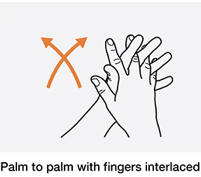
\includegraphics{images/dbs/1.png}
\caption{}
\end{figure}

\begin{itemize}
\tightlist
\item
  Prepare collection area. It should look like this:
\end{itemize}

\begin{figure}
\centering
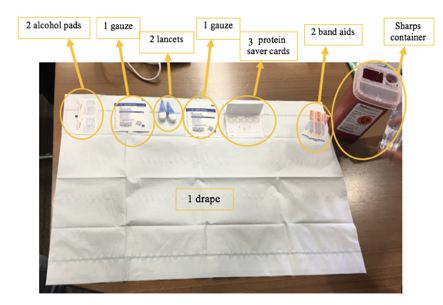
\includegraphics{images/dbs/2.png}
\caption{}
\end{figure}

\hypertarget{vr-headset-setup}{%
\subsubsection{VR Headset Setup}\label{vr-headset-setup}}

\begin{itemize}
\tightlist
\item
  Put VR goggles on for participant.
\item
  Ensure the headset has been charged before it needs to be used.
\item
  Bring the headset and the remote to the DBS Collection room.
\item
  Ask the subject if they are familiar with VR headsets, if they make them feel motion sick, and if they want to use the headset during the DBS protocol.
\item
  One of the RA's should pre-load the BABLab Youtube page:

  \begin{itemize}
  \tightlist
  \item
    Power on the headset (top center button on headset)
  \item
    Go to Library
  \item
    Select Youtube VR
  \item
    Go to the ``Account'' tab
  \item
    Go to the ``Liked Videos'' tab
  \end{itemize}
\item
  Show the child how the controller works:

  \begin{itemize}
  \tightlist
  \item
    moving your hand acts as the pointer/cursor
  \item
    to make selections, use the large bumper button on the back or press down the touchpad at the top of the controller
  \end{itemize}
\end{itemize}

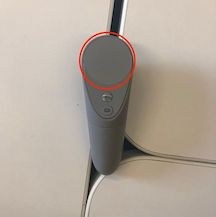
\includegraphics{images/dbs/3.jpeg} \emph{Touchpad}

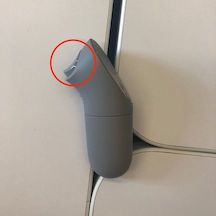
\includegraphics{images/dbs/4.jpeg} \emph{Back bumper}

\begin{itemize}
\tightlist
\item
  to scroll, move your finger up and down on the touch pad
\item
  to go back to the movie selection list, press the upper round button below the touchpad
\end{itemize}

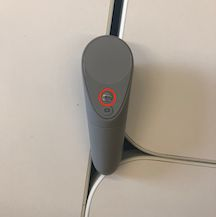
\includegraphics{images/dbs/5.jpeg} \emph{Back button}

\begin{itemize}
\tightlist
\item
  To put on the headset, loosen the side velcro straps and ask the child to hold the goggles in a comfortable position on their face. If the child wears glasses, they should be fine to use the headset while wearing them.
\item
  Tighten the straps so that the headset stays on its own but isn't uncomfortable for the child to wear.
\item
  Tell them they can watch any of the videos on the playlist.
\item
  Periodically check in with the child to ensure they aren't feeling motion sick or uncomfortable in any way.
\item
  After the DBS is completed, take the headset off the child and power it down.
\end{itemize}

\hypertarget{blood-sample-administration}{%
\subsubsection{Blood Sample Administration}\label{blood-sample-administration}}

\begin{itemize}
\tightlist
\item
  Place heating pad on participant's hand, making sure to cover fingers. Set to low or medium heat.

  \begin{itemize}
  \tightlist
  \item
    Check to make sure it does not get too hot.
  \item
    Set timer for 10 minutes.
  \end{itemize}
\item
  When 10 minutes are up, put on gloves. Have participant pull up heating pad and hold it with their free hand on the upper arm. Make sure the heating pad cable is not in the way of collection.
\item
  Clean middle or ring finger with alcohol and wipe with gauze.
\item
  Prick finger pad slightly off-center toward the side closest to the pinky finger and immediately dispose of lancet in sharps container.
\item
  Wipe first drop with gauze then start collecting on Whatman Protein cards in numbered order.
\item
  When finished, wipe with gauze, put pressure to stop bleeding and apply bandage.
\item
  Remove gloves, use hand sanitizer immediately, then wash hands ASAP.
\end{itemize}

\hypertarget{precautions}{%
\subsubsection{Precautions}\label{precautions}}

\begin{itemize}
\tightlist
\item
  Before, during and after the procedure, ask if the participant is feeling lightheaded.
\item
  Check the participant's complexion - turning pale is a warning sign for impeding faintness.
\item
  If participant feels faint/lightheaded, terminate the procedure, ask them to bend forward, and place their head between their knees. You may apply a cold compression to the back of the neck to speed up recovery.
\item
  Stay with them for at least 15 minutes until they feel completely fine.
\item
  Report the incident to Bridget.
\end{itemize}

\hypertarget{fainting-emergency}{%
\subsubsection{Fainting Emergency}\label{fainting-emergency}}

\begin{itemize}
\tightlist
\item
  In case of fainting or any warning symptoms, lay the participant down flat on a surface on their back and elevate their feet if possible (to a level higher than their heart, about 30cm).
\item
  Loosen any constrictive clothing/belts etc.
\item
  Symptoms usually disappear after a short rest.
\item
  If the participant does not regain consciousness within 1 minute, call 911.
\item
  If the participant regains consciousness, avoid having him/her get up too quickly.
\item
  Have them sit for at least 15 minutes until they feel completely fine.
\item
  Offer water or warm sweet drinks.
\item
  Report the incident to Bridget.
\end{itemize}

\hypertarget{biohazard-spill-emergency}{%
\subsubsection{Biohazard Spill Emergency}\label{biohazard-spill-emergency}}

\begin{itemize}
\tightlist
\item
  Equipments:

  \begin{itemize}
  \tightlist
  \item
    Disinfectant (Sodium Hypochlorite (Bleach))
  \item
    Absorbent materials sufficient to completely cover spilled liquid and can be disposed (e.g.~paper towels)
  \item
    Physical tools that allow safe handling of sharp materials (e.g.~tongs, forceps, broom/dustpan)
  \item
    Warning signs to notify others that a spill occurred in the area
  \end{itemize}
\item
  Check self for contamination and change PPE if necessary.
\item
  Put on new PPE to proceed with clean up.
\item
  Pick up broken glass/sharps with available physical tools and dispose as biohazardous sharps.
\item
  Place absorbent materials on and around spill.
\item
  Put disinfectant on paper towels and let it sit for at least 5 minutes.
\item
  Dispose of absorbent materials as biohazardous waste.
\item
  Repeat step 4-6 as necessary.
\item
  Remove PPE and wash hands with soap and water.
\item
  Report all spills to Bridget.
\end{itemize}

\emph{Note: Only proceed with biohazardous spill cleanup if you feel comfortable;
Always use physical tools for handling sharps.}

\hypertarget{incident-response-and-reporting}{%
\subsubsection{Incident Response and Reporting}\label{incident-response-and-reporting}}

An exposure incident is specific contact with hazardous agents. Exposure incidents at UCLA must be reported, investigated, and documented by UCLA Insurance \& Risk Management; Environment, Health \& Safety; and/or the supervisor of the facility.

\begin{itemize}
\tightlist
\item
  Notify all personnel in the room of the incident.
\item
  Move exposed individual(s) to a safe location, taking care to not spread biohazardous materials.
\item
  Remove contaminated clothing, turn exposed areas inward, and place in a leak-proof bag or container for future decontamination.
\item
  Wash skin with soap and water for 15 minutes.
\item
  Go directly to the Occupational Health Facility at 67-120 CHS (M-F, 7am-4pm) or the RRMC ER.
\item
  Notify Bridget ASAP.
\item
  Report the incident to EH\&S within 8 hours (24-hour hotline: 310-825-9797).
\item
  Record the incident in the Incident and Near Miss Log in the Biosafety Manual.
\end{itemize}

\emph{Note: Keep an extra set of clothes or shoes available to replace contaminated items.}

\begin{center}\rule{0.5\linewidth}{0.5pt}\end{center}

\hypertarget{protocol---child-questionnaires}{%
\subsection{Protocol - Child Questionnaires}\label{protocol---child-questionnaires}}

\begin{itemize}
\tightlist
\item
  Ask the participant how comfortable they are reading and comprehending in English
\item
  If not fully comfortable, read the questionnaires for the participant
\item
  Read the first questionnaire - the SS - to all participants
\end{itemize}

\hypertarget{children-8-under}{%
\subsubsection{Children 8 \& Under}\label{children-8-under}}

\begin{itemize}
\tightlist
\item
  The researcher will need to read all questions to child
\item
  PEDSQL GI \& PEDSQL F need the laminated face sheet
\end{itemize}

\begin{center}\rule{0.5\linewidth}{0.5pt}\end{center}

\hypertarget{protocols---post-session}{%
\section{Protocols - Post-Session}\label{protocols---post-session}}

\hypertarget{protocol---data-entry}{%
\subsection{Protocol - Data Entry}\label{protocol---data-entry}}

\begin{center}\rule{0.5\linewidth}{0.5pt}\end{center}

\hypertarget{protocol---data-quality-check}{%
\subsection{Protocol - Data Quality Check}\label{protocol---data-quality-check}}

\begin{center}\rule{0.5\linewidth}{0.5pt}\end{center}

\hypertarget{protocol---stool-sample-storage}{%
\subsection{Protocol - Stool Sample Storage}\label{protocol---stool-sample-storage}}

\hypertarget{training-video}{%
\subsubsection{Training Video}\label{training-video}}

\hypertarget{sample-quality}{%
\subsubsection{Sample Quality}\label{sample-quality}}

\begin{itemize}
\tightlist
\item
  Put on gloves.
\item
  Open the mailer to ensure that it contains both the stool sample (in biohazard bag) and the Bristol Stool Scale.
\item
  Check for quality of the stool sample by shaking it up and down vigorously (keep the sample in the biohazard bag), then check for its consistency and color - It should be a dark-brown liquid.
\item
  If stool sample does not meet requirement (e.g.~sample is in solid form or amount collected is too little), contact the family to see if they would be willing to send another sample with compensation.
\item
  Contact family if the Bristol Stool Scale is missing in the mailer.
\end{itemize}

\hypertarget{sample-transfer}{%
\subsubsection{Sample Transfer}\label{sample-transfer}}

\begin{itemize}
\tightlist
\item
  Wear appropriate PPE:

  \begin{itemize}
  \tightlist
  \item
    Gloves
  \item
    Lab coat
  \item
    Safety glasses
  \item
    Surgical Mask
  \item
    Closed-toe shoes
  \item
    Long pants
  \item
    Hair tied back
  \end{itemize}
\item
  Prepare your station and ensure that you have the following:

  \begin{itemize}
  \tightlist
  \item
    Drape
  \item
    2.0mL cryogenic vials
  \item
    Stool samples in biohazard bag
  \item
    Test tube racks
  \item
    Transport box with divider
  \item
    Sharpie for labeling
  \end{itemize}
\end{itemize}

\textbf{Steps:}

\begin{itemize}
\tightlist
\item
  Lay a new drape on the work station and keep all equipments and sample on the drape throughout the transfer process.
\item
  With the stool sample collection vial still in the biohazard bag, shake it up and down vigorously.
\item
  Take the stool sample out of the bag and put it on the test tube rack.
\item
  Untwist two 2.0mL vials and place them on the test tube rack.
\item
  Untwist the stool sample collection vial, and carefully pour the sample into the first 2.0mL vial. (It's okay if the ball does or does not get transferred)
\item
  Stop pouring when solution reached the 1.8mL line to prevent overflow, and pour the remaining sample (if any) in a second 2.0mL vial.
\item
  Cap the 2.0mL vials tightly to prevent spills.
\item
  Label the 2.0mL vials with a sharpie, ensure it has the participant ID and vial number.
\item
  Place the labeled 2.0mL vials in the transport box with divider.
\item
  Close the now-empty stool sample collection vial, put it back in the biohazard bag, and dispose it in the biohazard waste bin.
\item
  Clean up work station, dispose the drape, and wipe down the table top with disinfectant wipe.
\item
  Remove PPE and wash hands with soap and water thoroughly.
\item
  Bring the transport box to C454 where the -80˚C freezer is located (key in BABLab Lock Box).
\item
  Place the 2.0mL vials in their designated space in the freezer box (in accordance to the Sample Storage Log Diagram).
\item
  Log the sample in the \href{https://app.box.com/file/630322897864}{Sample Storage Log}.
\end{itemize}

\begin{center}\rule{0.5\linewidth}{0.5pt}\end{center}

\hypertarget{protocol---dbs-sample-storage}{%
\subsection{Protocol - DBS Sample Storage}\label{protocol---dbs-sample-storage}}

\begin{itemize}
\tightlist
\item
  Using a new drape, place the protein cards along the long horizontal midline of the drape.
\item
  Lightly fold the drape in half along the midline, covering the protein cards but ensure no contact between the drape and the blood spots (i.e.~ensure complete exposure of the blood spots).
\item
  Leave the protein cards to dry for 8-24 hours.
\item
  After drying, close the protein cards with the flap (make sure each one is labeled with wave \#, participant ID, date and card number), and place each card in a separate ziplock bag with a silica gel pack.
\item
  Place the bags in the BABLab freezer box in the -80˚C freezer in room C454 (key in BABLab lockbox).
\end{itemize}

\begin{center}\rule{0.5\linewidth}{0.5pt}\end{center}

\hypertarget{protocol---report-card-generation}{%
\subsection{Protocol - Report Card Generation}\label{protocol---report-card-generation}}

\begin{enumerate}
\def\labelenumi{\arabic{enumi}.}
\tightlist
\item
  Open a participant data folder
\end{enumerate}

\begin{figure}
\centering
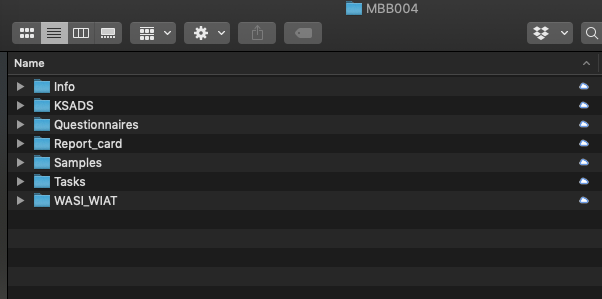
\includegraphics{images/final_checklist/report_cards/1.png}
\caption{}
\end{figure}

\begin{enumerate}
\def\labelenumi{\arabic{enumi}.}
\setcounter{enumi}{1}
\tightlist
\item
  Navigate to the report card folder and rename the template file - MBB999 to the relevant participant - and open the file
\end{enumerate}

\begin{figure}
\centering
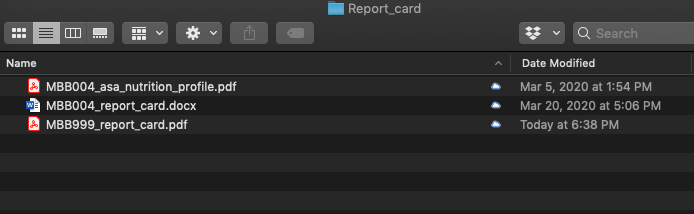
\includegraphics{images/final_checklist/report_cards/2.png}
\caption{}
\end{figure}

\begin{enumerate}
\def\labelenumi{\arabic{enumi}.}
\setcounter{enumi}{2}
\tightlist
\item
  If an ASA nutrition report has been generated for this participant, delete page 4 of the pdf. If no ASA nutrition report has been generated, delete page 3 of the pdf.
\end{enumerate}

\begin{figure}
\centering
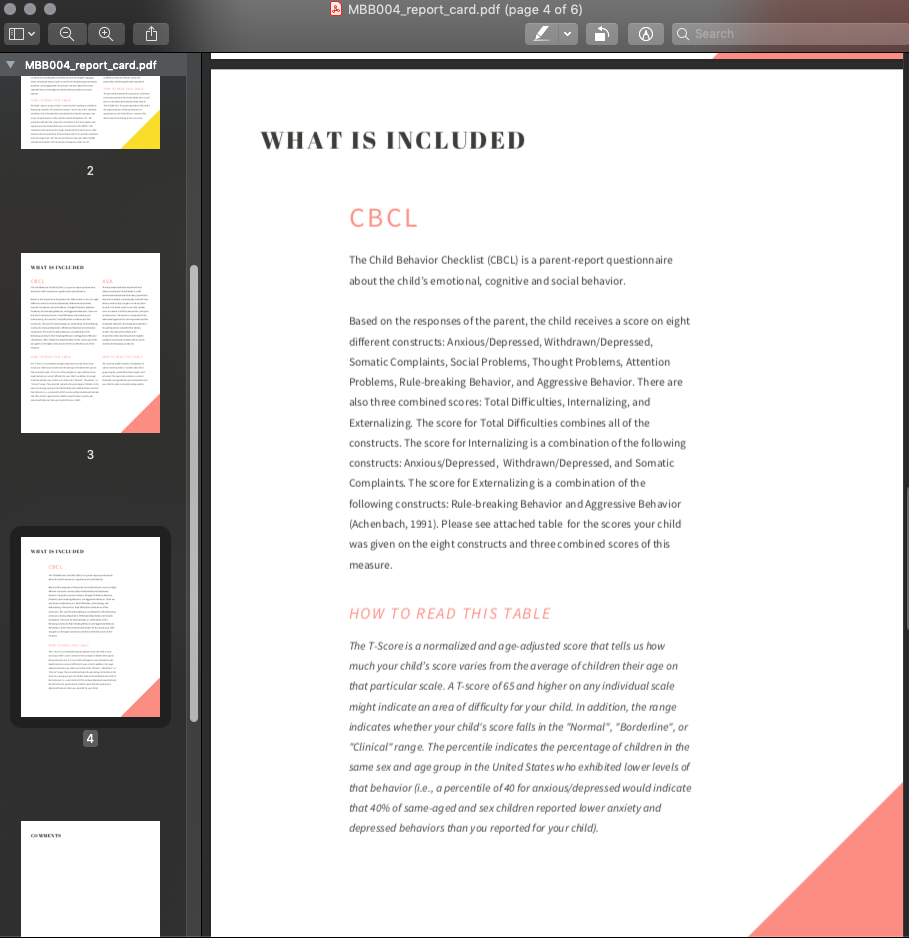
\includegraphics{images/final_checklist/report_cards/3.png}
\caption{}
\end{figure}

\begin{enumerate}
\def\labelenumi{\arabic{enumi}.}
\setcounter{enumi}{3}
\tightlist
\item
  Navigate to the last pge of the pdf, and fill in the scores for this participant. You can type directly on the page - it is a fillable form.
\end{enumerate}

\begin{figure}
\centering
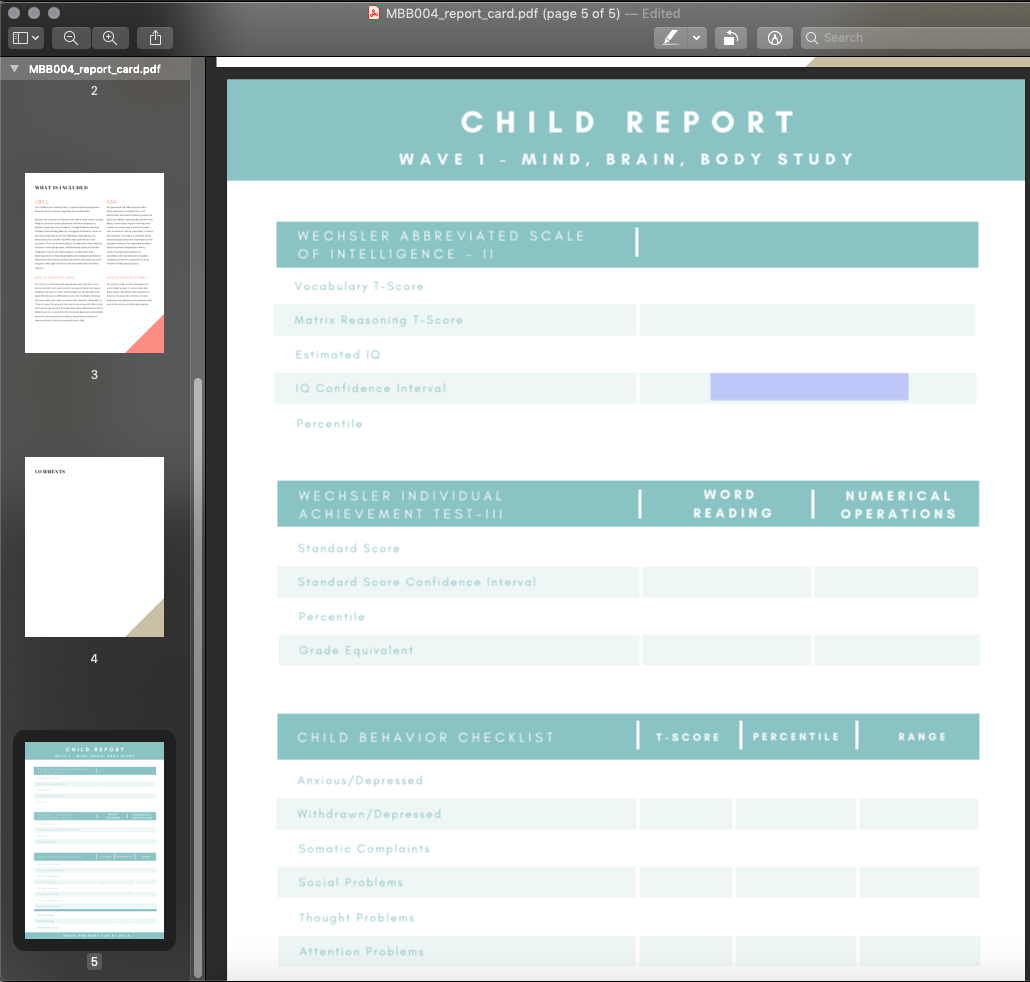
\includegraphics{images/final_checklist/report_cards/4.png}
\caption{}
\end{figure}

\begin{enumerate}
\def\labelenumi{\arabic{enumi}.}
\setcounter{enumi}{4}
\tightlist
\item
  After you have entered the data, it should look like this
\end{enumerate}

\begin{figure}
\centering
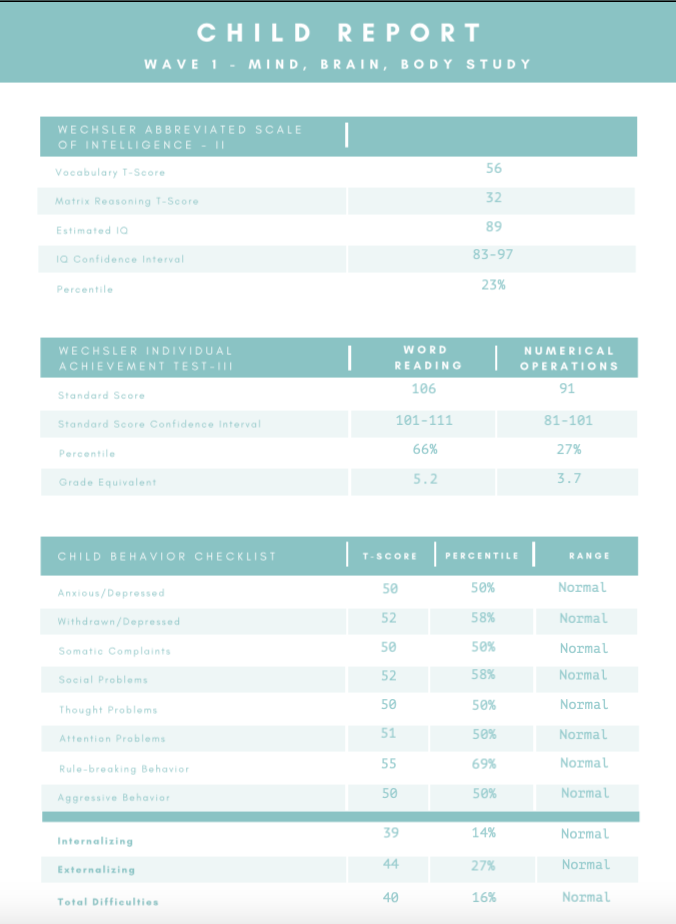
\includegraphics{images/final_checklist/report_cards/5.png}
\caption{}
\end{figure}

\begin{enumerate}
\def\labelenumi{\arabic{enumi}.}
\setcounter{enumi}{5}
\tightlist
\item
  If there are any comments, enter them on the comments page.
\end{enumerate}

\begin{itemize}
\item
  For example, if any NA's are present due to less than 70\% of data for that subset being available to calculate a score - note that here. Or, for example if the child was too young to receive a grade based score, you could note the aged based reading of the table here.
\item
  If there are no comments, delete this page.
\end{itemize}

\begin{figure}
\centering

\includegraphics{images/final_checklist/report_cards/6.png}
\caption{}
\end{figure}

\begin{enumerate}
\def\labelenumi{\arabic{enumi}.}
\setcounter{enumi}{6}
\tightlist
\item
  \textbf{Important} - Once you have completed the edits to the pdf, you must follow these steps to ``lock'' the data so that it is no longer editable before sending to the participant. To do so, click file/print/PDF/Save as PDF. Save the PDF to your desktop, then replace the original PDF with the desktop version.
\end{enumerate}

\begin{figure}
\centering
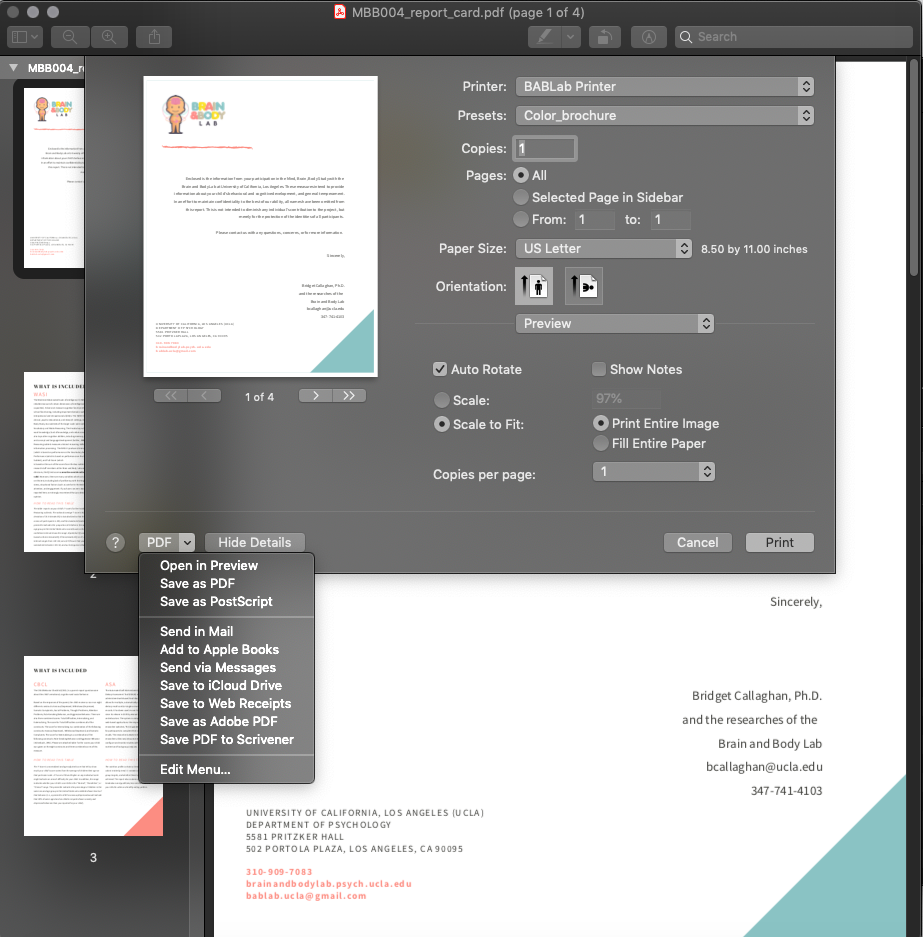
\includegraphics{images/final_checklist/report_cards/7.png}
\caption{}
\end{figure}

\begin{enumerate}
\def\labelenumi{\arabic{enumi}.}
\setcounter{enumi}{7}
\tightlist
\item
  The report card is now ready to be sent to the participant.
\end{enumerate}

\begin{center}\rule{0.5\linewidth}{0.5pt}\end{center}

\hypertarget{protocol---data-review-audit}{%
\subsection{Protocol - Data Review \& Audit}\label{protocol---data-review-audit}}

\hypertarget{follow-up-completed-by-scheduling-coordinator}{%
\subsubsection{Follow-Up (completed by Scheduling Coordinator)}\label{follow-up-completed-by-scheduling-coordinator}}

\begin{itemize}
\tightlist
\item
  Before sending Home Reminder 3, make sure RA's have completed Data Entry, Data Quality Check 1, and Data Quality Check 2.
\item
  After sending Home Reminder 3 - create blank Trello card for participant on \emph{In Data Review} list.
\end{itemize}

\hypertarget{data-review-completed-by-lab-manager-1}{%
\subsubsection{Data Review (completed by Lab Manager \#1)}\label{data-review-completed-by-lab-manager-1}}

\begin{itemize}
\tightlist
\item
  Once card has been created, do Data Review.
\item
  After completing Data Review, move card to \emph{Good Sample}, \emph{Bad Sample}, or \emph{No Sample} list based on the stool sample.
\end{itemize}

\hypertarget{data-audit-completed-by-lab-manager-2}{%
\subsubsection{Data Audit (completed by Lab Manager \#2)}\label{data-audit-completed-by-lab-manager-2}}

\textbf{If Good Sample:}

\begin{itemize}
\tightlist
\item
  Send payment, thank you letter, and certificate via mail.
\item
  Send {[}MBB - PAID{]} email and attach thank you letter, certificate, and report card (including outstanding items).
\item
  Move to \emph{Paid} list.
\item
  One week after payment is sent, check outstanding items do Audit Call \#1.
\item
  One week following Audit Call \#1, check outstanding items do Audit Call \#2.
\item
  Within 2 days, check outstanding items and do Audit Call \#3.
\item
  After Audit Call \#3 (or all items completed), send {[}MBB - DONE{]} email and move to \emph{Done} list.
\item
  If participant completes item on list, check card on Trello, mark off on participang log and data check sheets, and note in partipant's README in data folder.
\end{itemize}

\textbf{If Bad Sample:}

\begin{itemize}
\tightlist
\item
  Send payment, thank you letter, and certificate via mail. Include a new stool sample kit.
\item
  Send {[}MBB - PAID{]} email and attach thank you letter, certificate, and report card (including outstanding items - emphasize stool sample kit).
\item
  Move to \emph{Paid} list in Trello.
\item
  One week after payment is sent, check outstanding items do Audit Call \#1.
\item
  One week following Audit Call \#1, check outstanding items do Audit Call \#2.
\item
  Within 2 days, check outstanding items and do Audit Call \#3.
\item
  After Audit Call \#3 (or all items completed), send {[}MBB - DONE{]} email and move to \emph{Done} list.
\item
  If participant completes item on list, check card on Trello, mark off on participang log and data check sheets, and note in partipant's README in data folder.
\end{itemize}

\textbf{If No Sample:}

\begin{itemize}
\tightlist
\item
  Send {[}MBB - UNPAID{]} email and attach thank you letter, certificate, and report card (including outstanding items - emphasize stool sample kit).
\item
  Leave participant on Unpaid list.
\item
  If stool sample recieved - send payment, thank you letter, and certificate via mail and move to \emph{Paid} list.
\item
  If stool sample not received, one week after email is sent, check outstanding items do Audit Call \#1.
\item
  One week following Audit Call \#1, check outstanding items do Audit Call \#2.
\item
  Within 2 days of Audit Call \#2, check outstanding items and do Audit Call \#3.
\item
  After Audit Call \#3 (or all items completed), send {[}MBB - DONE{]} email and move to \emph{Done} list.
\item
  If participant completes item on list, check card on Trello, mark off on participang log and data check sheets, and note in partipant's README in data folder.
\end{itemize}

\begin{center}\rule{0.5\linewidth}{0.5pt}\end{center}

\hypertarget{wave-1-online}{%
\chapter{Wave 1 Online}\label{wave-1-online}}

\hypertarget{checklists-online}{%
\section{Checklists Online}\label{checklists-online}}

\begin{center}\rule{0.5\linewidth}{0.5pt}\end{center}

\hypertarget{checklist---initial-online}{%
\subsection{Checklist - Initial Online}\label{checklist---initial-online}}

\textbf{Scheduling and Confirmation}

\begin{itemize}
\tightlist
\item
  Schedule session 1 two weeks in advance from ``package mailing day'' (see package preparation in pre-session checklist)
\item
  Schedule session 2 \textasciitilde{}one week after session 1
\item
  Make Zoom link with scheduled session times and save to google calendar
\item
  Send session 1 confirmation email (in templates)

  \begin{itemize}
  \tightlist
  \item
    Attach \href{https://ucla.app.box.com/file/665452959932}{Next Steps}, \href{https://ucla.app.box.com/file/680632734387}{Computer Zoom Download Instructions}, and \href{https://ucla.app.box.com/file/680631353662}{Phone Zoom Download Instructions}
  \end{itemize}
\end{itemize}

\textbf{Enrollment}

\begin{itemize}
\tightlist
\item
  Create participant Box folder using MBB\_template (delete blank README from newly created folder)
\item
  Enroll participant in Wave 1 on REDCap
\item
  Fill participant instrument on REDCap
\item
  Fill counterbalance order on REDCap (Checklist - Lab Session Child Instrument)
\end{itemize}

\textbf{Calendar}

\begin{itemize}
\tightlist
\item
  Create MBB session calendar events (and invite researcher)

  \begin{itemize}
  \tightlist
  \item
    \emph{MBBXXX - Online Session 1}

    \begin{itemize}
    \tightlist
    \item
      Add \emph{Status: Incomplete} to the description
    \item
      Add \emph{Status Of Package: Not Received} to the description
    \end{itemize}
  \item
    \emph{MBBXXX - Online Session 2}

    \begin{itemize}
    \tightlist
    \item
      Add \emph{Status: Incomplete} to the description
    \item
      Add \emph{Session 2 Confirmation Email Sent: Incomplete} to the description
    \item
      Add \emph{Session 2 Links Email Sent: Incomplete} to the description
    \end{itemize}
  \end{itemize}
\item
  Create MBB mailing calendar event

  \begin{itemize}
  \tightlist
  \item
    \emph{MBBXXX - Mail Package}
  \end{itemize}
\item
  Create MBB reminder calendar events

  \begin{itemize}
  \tightlist
  \item
    \emph{MBBXXX - Session 1 Reminder 1 (email)} - 1 week prior
  \item
    \emph{MBBXXX - Session 1 Reminder 2 (email and call)} - 3 days prior
  \item
    \emph{MBBXXX - Session 2 Reminder 1 (email) } - 3 days before second session
  \item
    \emph{MBBXXX - Session 2 Reminder 2 (call)} - 2 days before second session
  \end{itemize}
\end{itemize}

\textbf{Reminders}

\begin{itemize}
\tightlist
\item
  Send \emph{Session 1 Reminder 1} email

  \begin{itemize}
  \tightlist
  \item
    In templates - attach next steps, consent/assent, zoom instructions, researcher information, ``What is involved in this study?'' video
  \item
    Confirm package is received
  \end{itemize}
\item
  Send \emph{Session 1 Reminder 2} email

  \begin{itemize}
  \tightlist
  \item
    In templates - attach previous
  \item
    Confirm package is received
  \end{itemize}
\item
  Confirm package is delivered and received
\item
  Confirm participant

  \begin{itemize}
  \tightlist
  \item
    Preferably by phone
  \item
    Update \emph{Session 1} calendar status
  \end{itemize}
\item
  Send \emph{Session 2 Reminder 1} email
\item
  Confirm participant

  \begin{itemize}
  \tightlist
  \item
    Preferably by phone
  \item
    Update \emph{Session 2} calendar status
  \end{itemize}
\end{itemize}

\begin{center}\rule{0.5\linewidth}{0.5pt}\end{center}

\hypertarget{checklist---pre-session-1}{%
\subsection{Checklist - Pre-Session 1}\label{checklist---pre-session-1}}

\hypertarget{package-preparation-magic-box}{%
\subsubsection{Package preparation: ``magic box''}\label{package-preparation-magic-box}}

\emph{(prepare and send from all scheduled participants in the last week, to be mailed 2 weeks prior to session)}

NOTE: Printing can be done in black and white.

\begin{itemize}
\tightlist
\item
  Print {[}What is in this magic box and what goes back to the lab?{]}
\item
  Print \href{https://ucla.app.box.com/file/668504120930}{Reward Board} (plus gold star stickers)
\item
  Print/Staple Parent Questionnaire Booklet (in this order)

  \begin{enumerate}
  \def\labelenumi{\arabic{enumi}.}
  \tightlist
  \item
    Parent Questionnaire Cover Page / Parent Proxy Intro
  \item
    demographics
  \item
    financial
  \item
    covid\_objective (parentproxy version)
  \item
    pedsql\_gi\_parentproxy
  \item
    pedsql\_wb\_parentproxy
  \item
    pedsql\_f\_parentproxy
  \item
    easy (revised)
  \item
    tesi (revised)
  \item
    cbcl (revised)
  \item
    cshq (revised)
  \item
    mb\_metadata
  \item
    med\_check
  \item
    pds
  \item
    dhws
  \item
    hpq
  \item
    parent\_stress
  \item
    cssi (for children under 8)
  \item
    fci (only adopted)
  \item
    iai (only internationally adopted)
  \item
    Parent Self Intro
  \item
    bdi
  \item
    covid\_objective (parentself version)
  \end{enumerate}
\item
  Print/Staple Session 1 Booklet (in this order)

  \begin{enumerate}
  \def\labelenumi{\arabic{enumi}.}
  \tightlist
  \item
    Session 1 Cover page
  \item
    \href{https://ucla.app.box.com/file/630327764749}{Pleasant/Unpleasant Events Checklist}
  \item
    \href{https://ucla.app.box.com/file/689385482411}{Height Measurement Instruction}
  \item
    \href{https://ucla.app.box.com/file/689387417719}{Weight Measurement Instruction}
  \item
    \href{https://ucla.app.box.com/file/689387420907}{Waist Measurement Instruction}
  \item
    Saliva Sample Instructions Sheet
  \item
    \href{https://ucla.app.box.com/file/685938821891}{Hair Sample Instructions Sheet}
  \end{enumerate}
\item
  Print/Staple Session 2 Booklet (in this order)

  \begin{enumerate}
  \def\labelenumi{\arabic{enumi}.}
  \tightlist
  \item
    Session 2 Cover Page
  \item
    \href{https://ucla.app.box.com/file/639652767665}{Contact List} and label with participant ID
  \item
    Stool Sample Instructions Sheet
  \item
    \href{https://app.box.com/file/630326499609}{Bristol Stool Scale} and label with participant ID (MBB Specific Version)
  \end{enumerate}
\item
  Prepare 2 sharpened pencils
\item
  Prepare paper measuring tape (for waist and height measurements)
\item
  Label 2 biohazard bags (with 2 cotton balls in each bag)
\item
  Label 1 cardboard box (for samples)
\item
  Label hair sample kit (aluminum foil 7``x7'', painter's tape with ``root end'' labeled, 1 ziplock bag pre-labeled with participant ID)
\item
  Label stool sample collection kit (paper clip collection tube and toilet hat together)
\item
  Label saliva sample collection kit (collection tube)
\item
  Insert MBB info card
\item
  Attach FedEx slip to return mailer
\item
  Label return mailer with ``exempt human specimen'' (in sharpie)
\item
  Take picture of prepaid blue return mailer (marked with MBB number) and file in participant data folder on Box
\item
  Insert all labeled items and forms for post-session in blue return mailer
\item
  Insert all labeled items and forms for session itself in magic box
\item
  Insert blue return mailer into study package
\item
  Tape package closed and put BABLAB sticker on
\item
  Take a picture of study package with tracking information to file on Box
\item
  Mail ``Magic Box'' package to participant
\end{itemize}

\begin{center}\rule{0.5\linewidth}{0.5pt}\end{center}

\hypertarget{setup---1-hour-prior}{%
\subsubsection{Setup - 1 Hour Prior}\label{setup---1-hour-prior}}

\begin{itemize}
\tightlist
\item
  Pull up session scripts/protocol
\item
  Activate the participant's ID on Gorilla
\item
  Prepare Session 1 checklist on google forms
\item
  Have the Participant's MBB and secondary MBB number on hand
\item
  Preload the Consent/Assent picture slideshow on researcher computer
\item
  Prepare biological sample kits for demonstration during session

  \begin{itemize}
  \tightlist
  \item
    hair sample, saliva sample, stool sample
  \end{itemize}
\item
  Ensure researcher's Zoom security settings are set for study session
\item
  Have the following links ready to send to the Participant throughout the session:

  \begin{itemize}
  \tightlist
  \item
    link to Consent on REDCap with codes ready
  \item
    link to Child's Gorilla Game
  \item
    link to child questionnaires on REDCap with codes ready
  \item
    link to COVID-19 Qualitative Responses on REDCap with codes ready
  \item
    Zoom link for Session 1
  \end{itemize}
\end{itemize}

\begin{center}\rule{0.5\linewidth}{0.5pt}\end{center}

\hypertarget{checklist---session-1}{%
\subsection{Checklist - Session 1}\label{checklist---session-1}}

\begin{itemize}
\tightlist
\item
  Session walk-through/package explanation
\item
  Consent/Assent
\item
  Parent-child observation (note recording via Zoom or pre-recording)
\item
  If pre-recorded, instruct participant how to upload to Box
\item
  Explain Questionnaires Parent Proxy or Parent self on second device if available (for parent to complete during Halloween training, Halloween test, and Child Questionnaires)
\item
  Halloween training
\item
  Height
\item
  Weight
\item
  Waist circumference
\item
  Halloween test
\item
  Saliva sample
\item
  Hair sample
\item
  Child Questionnaires
\item
  Qualitative parent and child free responses (optional)
\item
  Stool Sample explanation
\item
  Contact list explanation
\item
  Confirm mailing address for payment
\item
  Schedule time to complete post-session tasks \textasciitilde{}1 week post-session
\end{itemize}

\begin{center}\rule{0.5\linewidth}{0.5pt}\end{center}

\hypertarget{checklist---post-session-1}{%
\subsection{Checklist - Post-Session 1}\label{checklist---post-session-1}}

\hypertarget{notes}{%
\subsubsection{Notes}\label{notes}}

\begin{itemize}
\tightlist
\item
  Make note of issues to discuss (if needed) in Boxnote for next core meeting
\end{itemize}

\hypertarget{filing}{%
\subsubsection{Filing}\label{filing}}

\begin{itemize}
\tightlist
\item
  ``Scan'' Session 1 checklist and file in participant folder
\item
  Transfer and rename Zoom recording to Box
\item
  Download and copy behavioral task data (from Gorilla) to participant folder (raw)
\end{itemize}

\hypertarget{reminders}{%
\subsubsection{Reminders}\label{reminders}}

\begin{itemize}
\tightlist
\item
  Session 2 Confirmation Email sent with Zoom link, researcher info (right after Session 1)
\item
  Session 2 reminder 1 phone call made (day before Session 2)
\item
  Session 2 reminder 1 email sent with Zoom link (right before Session 2)
\end{itemize}

\begin{center}\rule{0.5\linewidth}{0.5pt}\end{center}

\hypertarget{checklist---session-2}{%
\subsection{Checklist - Session 2}\label{checklist---session-2}}

\begin{itemize}
\tightlist
\item
  Halloween test delay completed
\item
  Stool sample questions answered
\item
  Bristol Stool Scale reminder
\item
  Contact information sheet reminder
\item
  Walk through package to send back (check ``mbb\_online\_package\_checklists'') for checklist of items participant needs to send back to the lab
\end{itemize}

\begin{center}\rule{0.5\linewidth}{0.5pt}\end{center}

\hypertarget{checklist---final-online}{%
\subsection{Checklist - Final Online}\label{checklist---final-online}}

\hypertarget{filing-1}{%
\subsubsection{Filing}\label{filing-1}}

\begin{itemize}
\tightlist
\item
  Make low-res parent child interaction video and save on BABLab External Hard Drive
\item
  Burn all audio and video (low res) files to CD and label/store CD in binder
\item
  Make manila folder for participants to file all hard copies
\end{itemize}

\hypertarget{data-entry}{%
\subsubsection{Data Entry}\label{data-entry}}

\begin{itemize}
\tightlist
\item
  Enter online session checklist data to REDCap
\item
  Enter height, weight, waist to REDCap
\end{itemize}

\emph{After package has been received\ldots{}}

\hypertarget{package-confirmation}{%
\subsubsection{Package confirmation}\label{package-confirmation}}

\begin{itemize}
\tightlist
\item
  Halloween test delay completed
\item
  Hair sample received
\item
  Saliva sample received
\item
  Stool sample received
\item
  Bristol Stool Scale data received
\item
  Questionnaires received (if paper versions were sent)
\item
  Consent/Assent forms received (if paper versions were sent)
\item
  Contact information sheet received
\end{itemize}

\hypertarget{data-entry-1}{%
\subsubsection{Data Entry}\label{data-entry-1}}

\begin{itemize}
\tightlist
\item
  Enter contact list information into recruitment database
\item
  Enter questionnaires data (if paper versions were sent)
\item
  Scan and upload Bristol Stool Scale to Box
\item
  Enter Bristol Stool Scale data to REDCap
\end{itemize}

\hypertarget{filing-2}{%
\subsubsection{Filing}\label{filing-2}}

\begin{itemize}
\tightlist
\item
  File Consent/Assent forms in filing cabinet (consent manila folder)
\item
  File contact list in filing cabinet (contact list manila folder)
\item
  File Bristol Stool Scale in filing cabinet (participant folder)
\item
  File questionnaires in filing cabinet if paper versions were sent (participant folder)
\end{itemize}

\hypertarget{sample-storage}{%
\subsubsection{Sample Storage}\label{sample-storage}}

\begin{itemize}
\tightlist
\item
  Label and store stool sample (add data quality to REDCap)
\item
  Label and store saliva sample
\item
  Label and store hair sample
\item
  Update sample storage log on Box (once all received)
\item
  Upload all sample photos to Box
\end{itemize}

\hypertarget{data-quality}{%
\subsubsection{Data Quality}\label{data-quality}}

\begin{itemize}
\tightlist
\item
  Data quality check 1
\item
  Data quality check 2
\item
  Data review
\item
  Data audit
\end{itemize}

\hypertarget{retention}{%
\subsubsection{Retention}\label{retention}}

\begin{itemize}
\tightlist
\item
  Prep report card
\item
  Send report card email (in templates - attach report card)
\item
  Update participant Wave 2 status
\end{itemize}

\hypertarget{reimbursement}{%
\subsubsection{Reimbursement}\label{reimbursement}}

\begin{itemize}
\tightlist
\item
  Mail payment with science kits
\item
  Take a picture of tracking information and upload to Box
\item
  Log participant payment in reimbursement log book
\item
  Log participant payment in reimbursement spreadsheet
\item
  Send payment confirmation email to participant
\end{itemize}

\begin{center}\rule{0.5\linewidth}{0.5pt}\end{center}

\hypertarget{protocols---pre-session-1}{%
\section{Protocols - Pre-Session 1}\label{protocols---pre-session-1}}

\hypertarget{protocol---recruitment-online}{%
\subsection{Protocol - Recruitment Online}\label{protocol---recruitment-online}}

\hypertarget{pre-screening}{%
\subsubsection{Pre-Screening}\label{pre-screening}}

\begin{enumerate}
\def\labelenumi{\arabic{enumi}.}
\tightlist
\item
  Check if participant is in Recruitment Database

  \begin{itemize}
  \tightlist
  \item
    If not, add them to the Recruitment Database
  \end{itemize}
\item
  Check if participant is in ID Drive

  \begin{itemize}
  \tightlist
  \item
    If yes, check if they have a Screener ID
  \item
    If not, assign them a Screener ID once contact has been established based on the next available Screener ID \# in REDCap and proceed with screening
  \item
    If yes, proceed with screening under existing Screener ID in REDCap
  \end{itemize}
\end{enumerate}

\hypertarget{screening}{%
\subsubsection{Screening}\label{screening}}

\begin{enumerate}
\def\labelenumi{\arabic{enumi}.}
\tightlist
\item
  To screen a new participant click ``Add / Edit Records''
  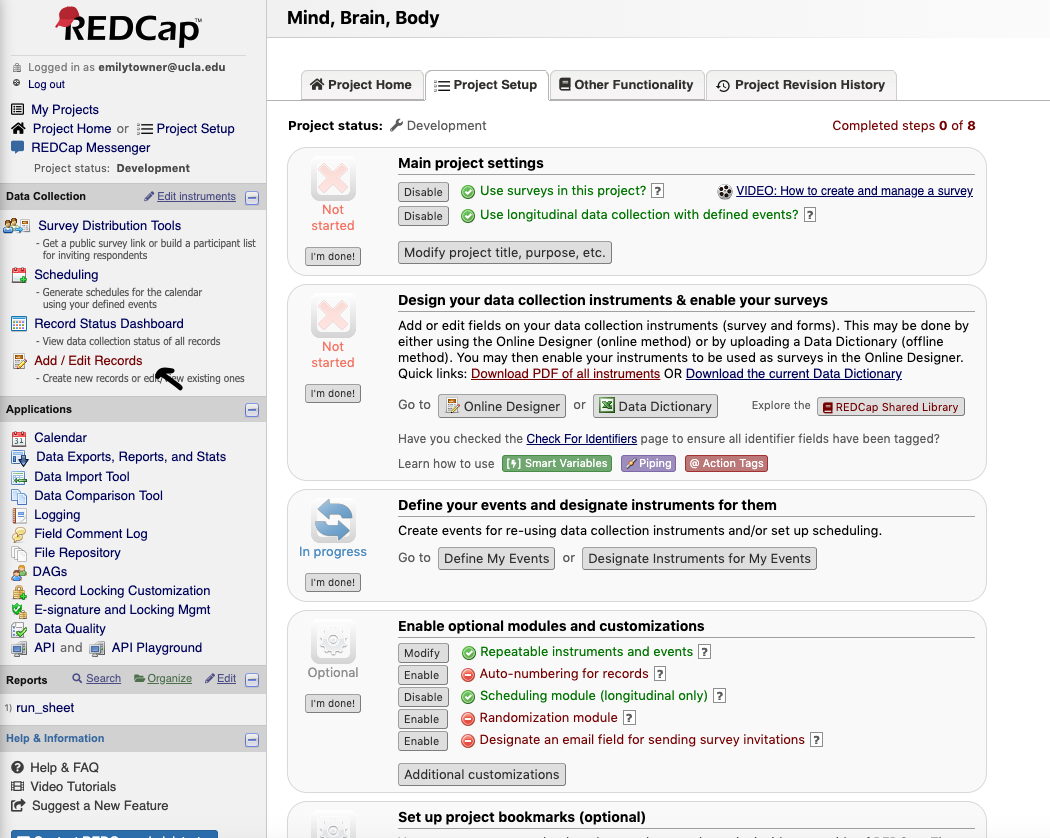
\includegraphics{images/redcap_screening/1.png}
\item
  Click to enter a new Subject ID

  \begin{itemize}
  \tightlist
  \item
    Make sure Arm 1: Recruitment is selected
  \end{itemize}
\item
  Type ``SMBB\#'' (Screener ID) to create a record and hit ``Enter''

  \begin{itemize}
  \tightlist
  \item
    Make sure to link the participants Screener ID and their name on the \textbf{ID Drive ONLY}
  \item
    Before creating a new record, be sure to check the ID Drive to see if the participant already has an existing Screener ID
  \item
    If a record exists, add a new instance of the screen instead of creating a new record
    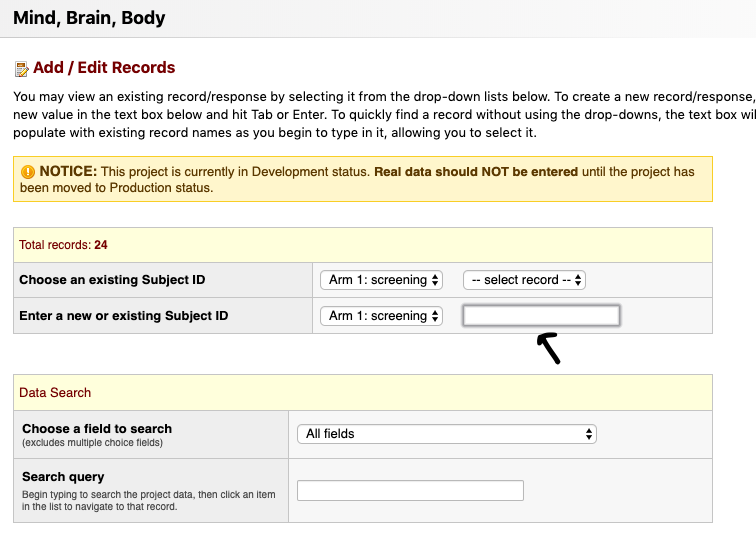
\includegraphics{images/redcap_screening/2.png}
  \end{itemize}
\item
  The screening arm contains two parts

  \begin{itemize}
  \tightlist
  \item
    The screen
  \item
    The wave1\_status

    \begin{itemize}
    \tightlist
    \item
      The wave1\_status is to be updated after the first and each subsequent contact
      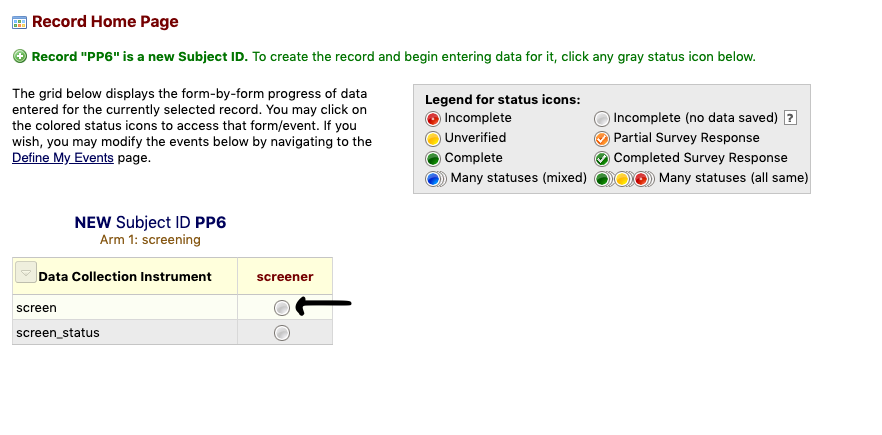
\includegraphics{images/redcap_screening/3.png}
    \end{itemize}
  \end{itemize}
\item
  Click on the radio button in the ``screen'' row to screen the participant
  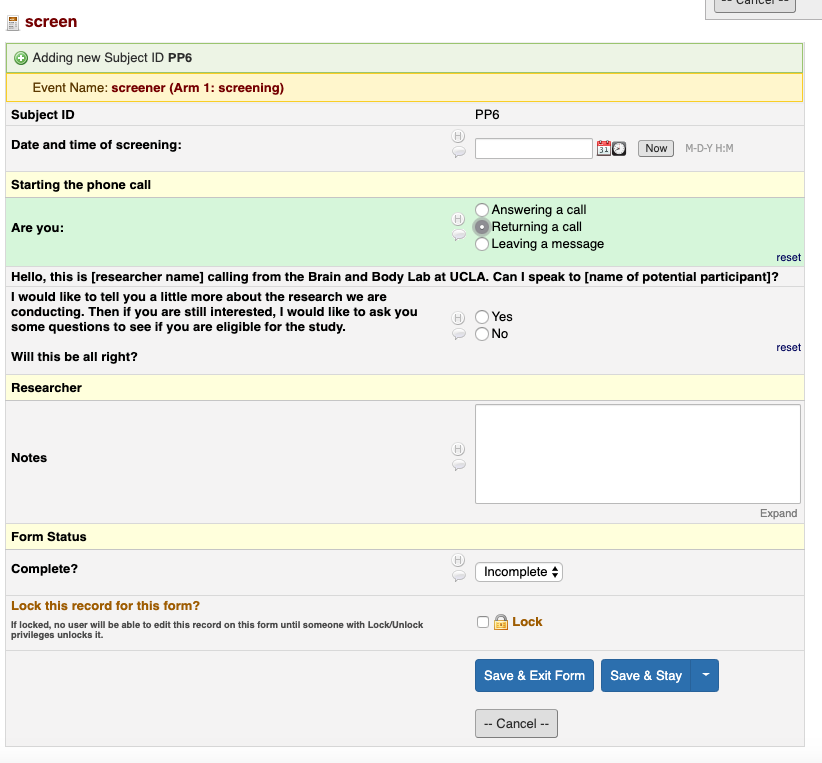
\includegraphics{images/redcap_screening/4.png}
\item
  Click ``Now'' to enter today's date and time
\item
  Select the appropriate choice to start the phone call and follow the skip logic
\item
  Follow the skip logic to the end

  \begin{itemize}
  \tightlist
  \item
    For items without a text field, write the information down in the Recruitment database (This identifying information cannot be on REDCap)
  \end{itemize}
\item
  Once done, select ``Complete'' and ``Save \& Exit Form''

  \begin{itemize}
  \tightlist
  \item
    The screen can be entered multiple times - for instance if there are multiple phone calls or contacts
  \item
    It is important to keep a record of all instances of contact
    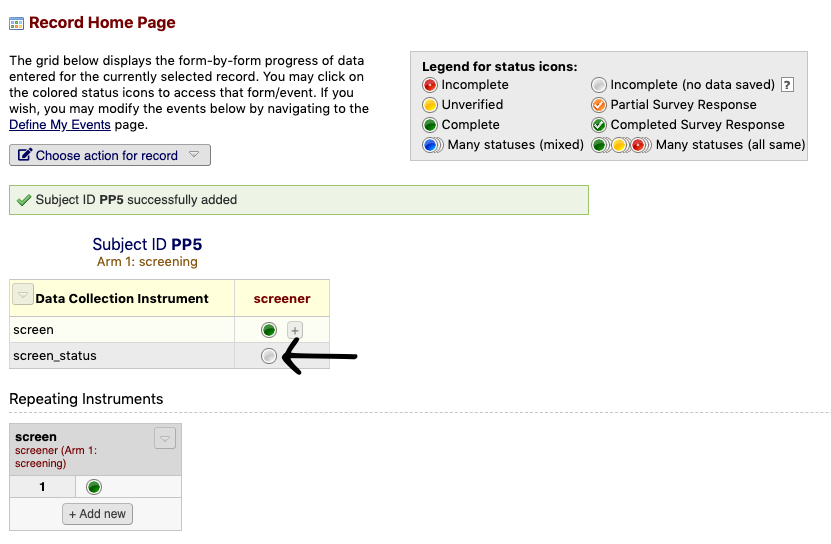
\includegraphics{images/redcap_screening/5.png}
  \end{itemize}
\item
  Click the screen\_status radio button
  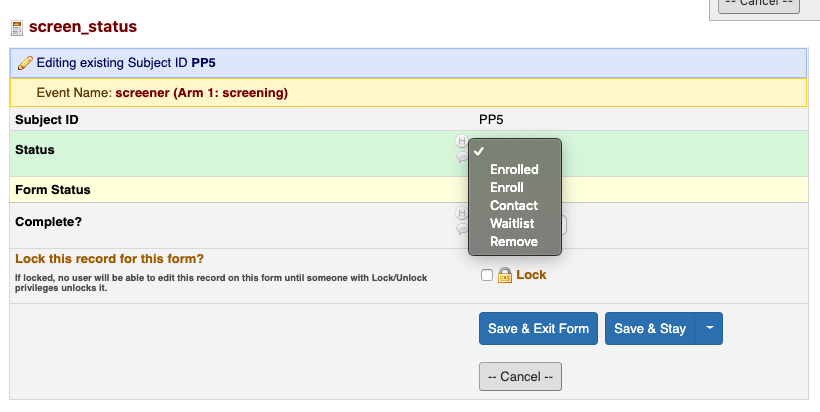
\includegraphics{images/redcap_screening/6.png}
\item
  Select the appropriate option

  \begin{itemize}
  \tightlist
  \item
    Contact - Participant needs to be re-contacted (add Recruitment Database \& ID Drive)
  \item
    Ineligible - Participant not eligible for study
  \item
    To Enroll - Participant to enroll (need to create subject ID, enter subject info, schedule participant, add to Recruitment Database, add to ID Drive)
  \item
    Enrolled - Participant has been enrolled (all above have been completed)
  \item
    To Remove - Participant wants to be removed
  \end{itemize}
\item
  Be sure to update the screen status after each contact

  \begin{itemize}
  \tightlist
  \item
    After 3 contacts (with no response) - review (time of day, contact method, etc.)
  \end{itemize}
\item
  If enrolled, proceed to pre-session checklist in the participant log
\end{enumerate}

\hypertarget{scheduling}{%
\subsubsection{Scheduling}\label{scheduling}}

\begin{enumerate}
\def\labelenumi{\arabic{enumi}.}
\tightlist
\item
  Open BabLab google calendar and note availability for designated data collection research team.
\item
  Check-in with the Lab Manager to see what the designated ``package mailing day'' of the week is.
  Participants must be scheduled 2 weeks or more in advance from the ``package mailing day'', to ensure appropriate time for the package to be received by the participant.
\item
  Create event on google calendar for 2 hours. Notify the participant that sessions may not last the full indicated time, however, we like to designate additional time just in case.
\item
  As soon as the participant has been scheduled, create/add to a google calendar event for the designated ``package mailing day'' of the week the participant ID (MBB number).
\item
  This will notify the Lab Manager to create a package for this participant with session and post-session materials when they go into the lab for ``package mailing day.''
\end{enumerate}

Making a Zoom link

\begin{enumerate}
\def\labelenumi{\arabic{enumi}.}
\tightlist
\item
  Log onto \url{https://zoom.us}
\item
  Click to ``Meetings'' and ``Schedule a new meeting'' 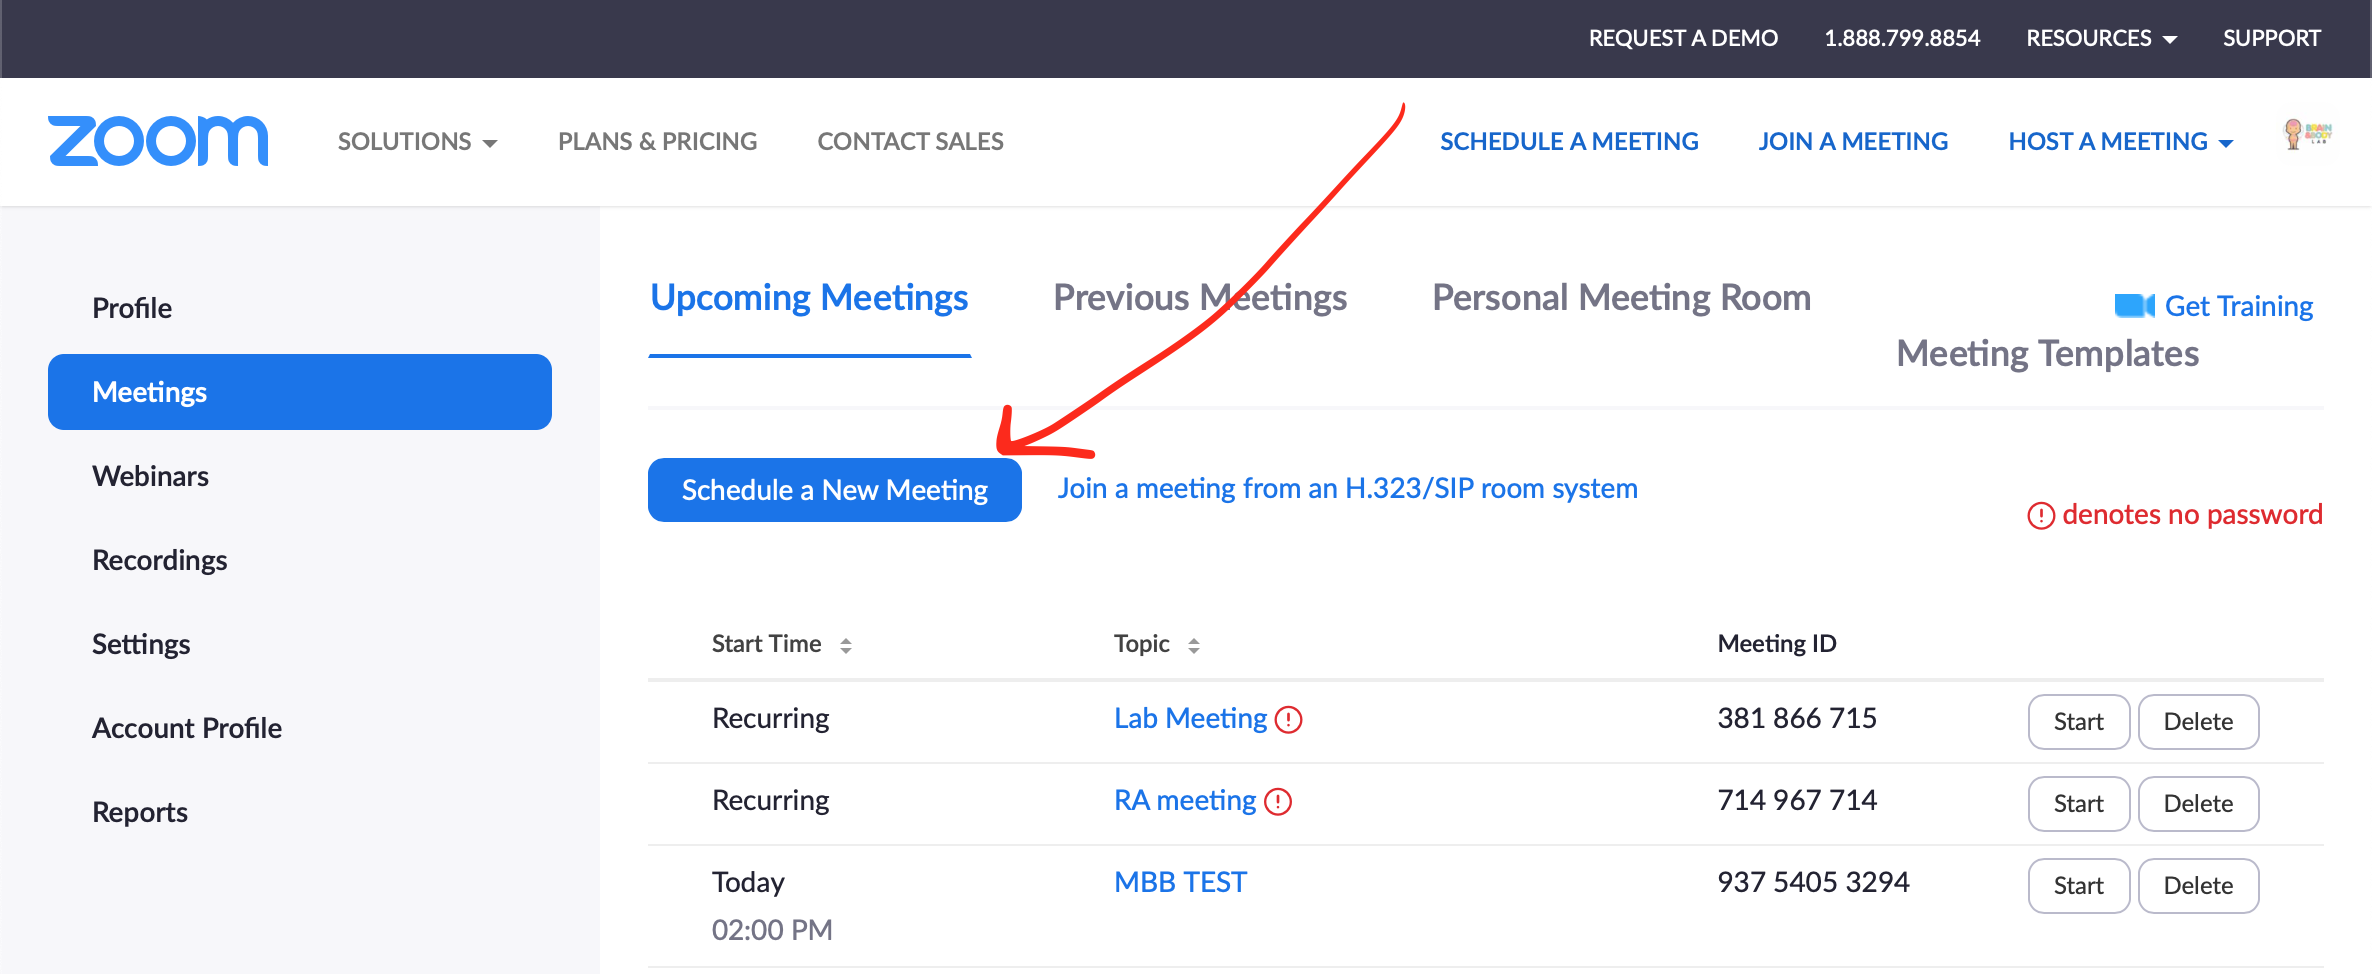
\includegraphics{images/zoom_link/1.png}
\item
  Title the meeting with the Participant's MBB number, set scheduled time, indicate 3 hours 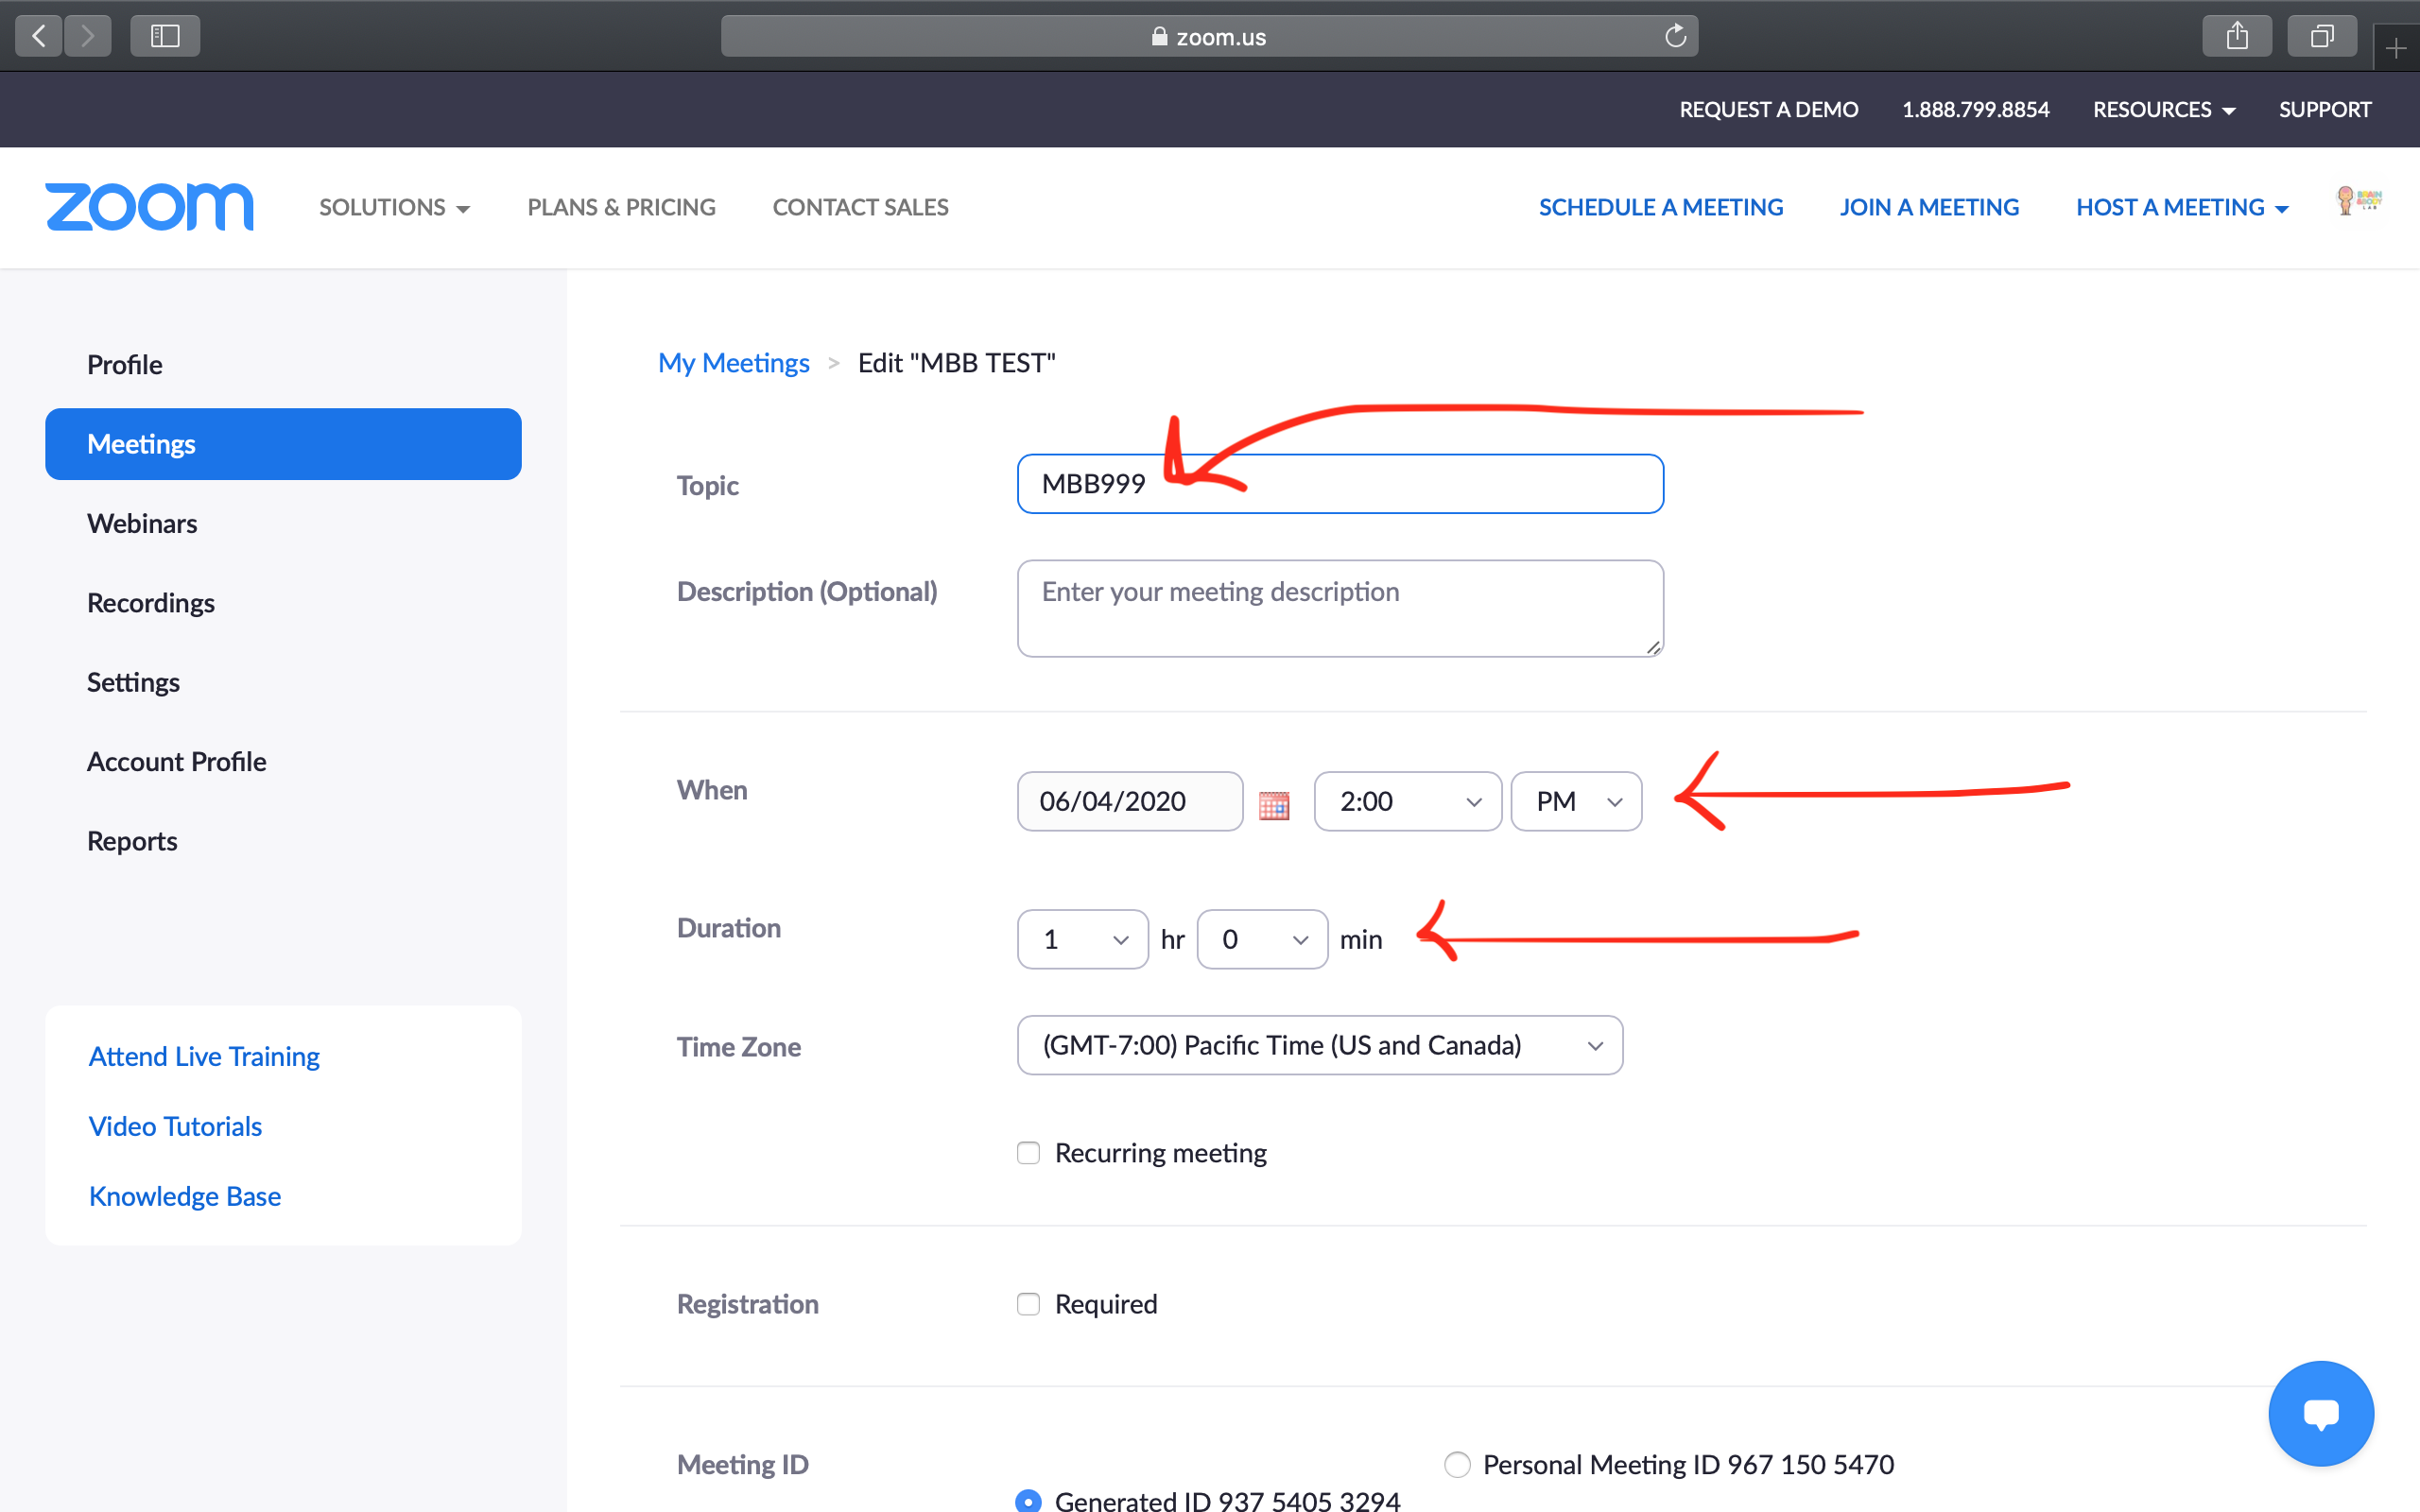
\includegraphics{images/zoom_link/2.png}
\item
  Set setting with password and turn host/participant on \includegraphics{images/zoom_link/3.png}
\item
  Save and click to add Zoom meeting to google calendar \includegraphics{images/zoom_link/4.png}
\item
  Click on the \href{mailto:bablab.ucla@gmail.com}{\nolinkurl{bablab.ucla@gmail.com}} \includegraphics{images/zoom_link/5.png}
\item
  Click allow \includegraphics{images/zoom_link/6.png}
\item
  Copy the Zoom link from the Description section and save \includegraphics{images/zoom_link/7.png}
\item
  Paste Zoom link into the ``confirmation email'' you send to the participant with their session confirmation, Zoom instruction sheet, and Next Steps sheet
\end{enumerate}

\hypertarget{other-screening-information}{%
\subsubsection{Other Screening Information}\label{other-screening-information}}

Accessing Lists

To find out where participants are in the recruitment process, there are several lists.
\includegraphics{images/redcap_screening/7.png}
1. Click on ``Record Status Dashboard''
\includegraphics{images/redcap_screening/8.png}
2. Participants who have been enrolled will be listed in the Enrollment - Wave 1 list
3. Participants in the process of recruitment will be listed in one of the 4 Recruitment lists
- *These lists are populated based on the individuals ``Screen Status'' so be sure to update after each contact!

List Types

\begin{itemize}
\tightlist
\item
  Contact - List of individuals who need to be contacted or re-contacted (also includes waitlist)
\item
  Ineligible - Participants are ineligible but interested
\item
  To Enroll - Participants who have been screened and are eligible to enroll
\item
  To Remove - Participants who were not interested in being contacted for this or future research
\end{itemize}

\hypertarget{concerns}{%
\subsubsection{Concerns}\label{concerns}}

If a parent has a concern about the study before the session, send the email template:

\begin{itemize}
\tightlist
\item
  {[}MBB\_online - CONCERNS{]}
\end{itemize}

\begin{center}\rule{0.5\linewidth}{0.5pt}\end{center}

\hypertarget{protocol---session-preparation}{%
\subsection{Protocol - Session Preparation}\label{protocol---session-preparation}}

\hypertarget{package-creation}{%
\subsubsection{Package creation}\label{package-creation}}

\begin{itemize}
\tightlist
\item
  There will be a designated ``package mailing day'' one day a week in which the Lab Manager will go into the lab to prepare necessary materials and send out packages from scheduled participants in the last week, on the same package mailing day.
\item
  Once the package has been put together, it is time to bring the package down to Tyler's office in the Psychology building OR to the UCLA MDDS.
\item
  To mail the package to the participant, you will need the following information:

  \begin{itemize}
  \tightlist
  \item
    Recharge ID
  \item
    Participant name
  \item
    Participant mailing address
  \end{itemize}
\item
  From Tyler's office, you will receive a FedEx label in which you can write this information
\item
  At MDDS, they will package your materials for you.
\item
  Take a picture of the FedEx label and upload to Box
\item
  Leave the package in Tyler's office for FedEx pickup/MDDS to mail out
\end{itemize}

\hypertarget{zoom-security-settings}{%
\subsubsection{Zoom security Settings}\label{zoom-security-settings}}

\begin{enumerate}
\def\labelenumi{\arabic{enumi}.}
\tightlist
\item
  Require Encryption for 3rd Party Endpoints*
\item
  Prevent participants from saving chat
\item
  Click on the ``security'' button and ensure the following items are checked and all other items unchecked \includegraphics{images/zoom_security/1.png}

  \begin{enumerate}
  \def\labelenumii{\alph{enumii}.}
  \tightlist
  \item
    ``Enable Waiting room''
  \item
    ``Lock Meeting'' after participant has entered
  \item
    Allow participant to ``Unmute Themselves''
  \end{enumerate}
\item
  Disable Cloud recording*
\item
  Host-only screen-sharing

  \begin{enumerate}
  \def\labelenumii{\alph{enumii}.}
  \tightlist
  \item
    click on the arrow next to ``screen sharing'' and click on ``Advanced sharing options'' \includegraphics{images/zoom_security/2.png}
  \item
    Ensure ``one participant can share at a time'' and ``only host'' options are selected \includegraphics{images/zoom_security/3.png}
  \end{enumerate}
\end{enumerate}

*Note that \#1 and \#4 are the default settings (so those don't have to be changed).

\hypertarget{activating-participant-on-gorilla}{%
\subsubsection{Activating participant on Gorilla}\label{activating-participant-on-gorilla}}

\begin{enumerate}
\def\labelenumi{\arabic{enumi}.}
\tightlist
\item
  Log in to Gorilla
\item
  Navigate to Projects/MBB/MBB\_wave\_1\_online
\item
  Navigate to the participants tab
\item
  Click ``Activate'' for the designated participant
\end{enumerate}

\begin{figure}
\centering
\includegraphics{images/gorilla/1.png}
\caption{}
\end{figure}

\begin{figure}
\centering
\includegraphics{images/gorilla/2.png}
\caption{}
\end{figure}

\begin{figure}
\centering
\includegraphics{images/gorilla/3.png}
\caption{}
\end{figure}

\begin{figure}
\centering
\includegraphics{images/gorilla/4.png}
\caption{}
\end{figure}

\begin{figure}
\centering
\includegraphics{images/gorilla/5.png}
\caption{}
\end{figure}

\begin{center}\rule{0.5\linewidth}{0.5pt}\end{center}

\hypertarget{protocols---session-1}{%
\section{Protocols - Session 1}\label{protocols---session-1}}

\hypertarget{protocol---consent-assent-online}{%
\subsection{Protocol - Consent \& Assent Online}\label{protocol---consent-assent-online}}

{[}ONCE ZOOM IS CONNECTED{]}

\emph{Hi! Thank you so much for joining us today! We are so looking forward to today's session with you. Usually, when we conduct a study such as this, we would do it our lab at UCLA. However, with COVID-19 we've decided it would be safer to carry out this study online for the time being- social distancing and all!}

\emph{Our session today should take around 1 hour long. In addition to what we do here today, there will be a follow up zoom appointment with us one week from now. At that appointment, we will reconnect on a second Zoom call in which your child will log on for 10 minutes and complete a computer game.}

\emph{Sounds good? Let's get started!}

{[}Researcher to open up the \href{https://ucla.app.box.com/file/689404174873}{MBB\_Consent\_Script\_Presentation}{]}

\emph{First thing we are going to do is go over what is on the consent and assent forms. (These are the attached documents we sent you in the emails leading up to this session.) We will walk through, in a little bit more detail, all of the things we will be doing during today's session.}

\emph{During today's online session we are going to be doing some interactive things. First, we are going to have you and your parent sit and talk about some fun things and some not so fun things while on ZOOM. This conversation will be recorded but we will not be watching or listening in}

\emph{Next, we are going to have you play a game on the computer. In this game, you will be looking at pictures. Some of the pictures will be a bit scary, some sad, others a bit boring. While you are playing this game, your parent will stay with you in the room but will be working on some surveys to fill out.}

\emph{After the game is over, your parent {[}NAME{]} will help measure your height, weight, and waist circumference.}

\emph{You will also be answering some surveys (for children) with the researcher OR (for teens) on your own.}

\emph{Lastly for today, your parent will help take two biological samples during this session.}

\begin{enumerate}
\def\labelenumi{\arabic{enumi}.}
\tightlist
\item
  One is the hair sample which helps measure hormones that everyone has in their hair
\item
  Two is the saliva sample which helps tell us learn a little bit more about your microbiome
\end{enumerate}

\begin{itemize}
\tightlist
\item
  Do you know what a microbiome is?
\item
  A microbiome is all the little bacteria that live inside your mouth. Everyone has these, they are healthy! We just want to know what kind and how many of each there are.
\end{itemize}

\emph{For helping us out in today's session, you will be getting \$45 for the work you put in! After this online session is over, we'll ask you to do three more things at home:}

\begin{enumerate}
\def\labelenumi{\arabic{enumi}.}
\tightlist
\item
  One is the Child poop sample -- this helps us learn a bit more about your microbiome
\end{enumerate}

\begin{itemize}
\tightlist
\item
  There are also little bacteria that live in your tummy! Everyone has these and we want to know more about them.
\end{itemize}

\begin{enumerate}
\def\labelenumi{\arabic{enumi}.}
\setcounter{enumi}{1}
\tightlist
\item
  Two is filling out the stool scale -- this is a short scale that gives a description of your sample
\item
  Three is the computer memory game -- this is when you will log back on with us via ZOOM in a week's time to see what you remember from today's session
\end{enumerate}

\emph{Great! Do you have any questions for us about any of the samples}

\emph{When you complete the poop sample and the computer game at home, we will pay you another \$20!}

\emph{We will send the full payment of \$65 (\$45 for today's session and \$20 for completing the home session) as soon as we receive the samples back through the mail.}

\emph{Here are some things to keep in mind:}

\emph{You are a volunteer in this study, which means you do not have to do anything, or say anything, that makes you uncomfortable. We would like you to try everything you can, and to do your best, but if there are things you absolutely do not want to do, just tells us, that is o.k.}

\emph{We will keep your participation confidential. You are given an ID number in order to keep your data confidential and separated from your name. Therefore, any identifying information (like your name, email, address, etc.) will be kept private and not paired with your data. We will also use a secondary ID number to save the videos with (since your faces are in it), which will help separate this from your name and the other data we collect form you. Only members of our research team will have access to your name and ID numbers.}

\emph{I will rename your ``ZOOM Name'' right now with your Secondary ID number, to prepare for the recordings we will take in our session today}

{[}Researcher will rename the participant's name to the participant Secondary MBB ID number. \includegraphics{images/zoom_parent_child_interaction/1.png}

\emph{As this is a longitudinal study, and we want you to come again in the future if you are interested, we will ask for some information so that we may reach out to you in the future. Do you have any questions?}

\emph{Ok- I will now send you a link through the Zoom chat, which will open up a survey that allows you to virtually indicate your consent to participate in the study. If you'd like, you can share your screen with us now and we can walk you through it. Once you get that pulled up, you will see the consent/assent documents attached there as well- please feel free to take your time reading through the consent and assent forms now if you'd like. As I mentioned earlier, these are the documents we had previously sent you in the emails leading up to today's session.}

{[}Then once they are done reading through{]}

\emph{All set and any questions?}

{[}IF NO,{]} \emph{Please click to indicate your consent/assent and submit the REDCap form. You may press submit once you are finished to ``send in the form.''}

Researcher to grab magic box.

\emph{Once you are all set with that, we'd like you for to grab the magic box we sent you in the mail. This contains everything you will need for today's session and what you will do at home after today's session.}

\emph{If you haven't already done so, please open the magic box up. The magic box should contain a sheet of paper at the top which details all of the contents, but we will let you know when you need to take each item out of the box. Please set aside the magic box for now but keep the materials near you as we may need to access materials from the magic box throughout today's session!}

\emph{What you can pull out now and use throughout the session is the Reward Board and Gold Star Stickers. Use this reward board to track all the steps you accomplish today! Each space is like each task for the session. Once you complete the task you can put a gold star on the space!}

\emph{Are you ready to get started on the session? Great, lets dive in!}

\begin{center}\rule{0.5\linewidth}{0.5pt}\end{center}

\hypertarget{protocol---parent-child-observation-online}{%
\subsection{Protocol - Parent Child Observation Online}\label{protocol---parent-child-observation-online}}

The parent and child will be seated together in view on the Zoom camera. During that time they will be filmed while solving a conflict, and then again while discussing a pleasant event. The conflict event will always go first, followed by the pleasant event. We did this to ensure that the parents were not thinking of the negative interaction upon answering the questionnaires about their child, which they did immediately after the observation interaction.

Step 1:
The researcher will ask the parent to find the \href{https://ucla.app.box.com/file/630327764749}{Pleasant/Unpleasant Events Checklist} piece of paper from their session package.

\emph{Researcher: So the first thing we will have you pull out of the magic box is the paper packet titled ``Online Session Booklet.'' You can flip to the page that says ``Pleasant Events and Issues Checklist.''}

Researcher will wait for the participant to find the Online Session Booklet and flip to the correct page.

\emph{Researcher: Next we are going to take some film of you while you discuss something that's hard and try to resolve it. On this piece of paper (Issues Cheklist) is a list of things that parents and children sometimes have disagreements about. We will give you a moment to read the list and think about some that you would like to discuss together. Then after about one minute, you will start discussing the things you have selected and try to resolve them. You do not need to tell us what you chose to discuss, and it does not matter if you chose something from this list, or decide to choose something else. I'll be there while you choose, but once your five minute discussion starts, I am going to turn off my camera and mute myself to be out of the recording. When you are ready, I will begin the recording and give you a minute or so to choose. Then, I will let you know when to start discussing for five minutes! Are you ready?}

Step 2:
- Researcher will ensure Zoom security settings are set up for the video.
- Parent and child will be situated side-by-side in view on the Zoom camera.
-Researcher will press record on the Zoom application. \includegraphics{images/zoom_parent_child_interaction/3.png} Wait to hear the audio Zoom confirmation \emph{``this meeting is now being recorded''} and view recording in progress at top left of screen to ensure recording is live. \includegraphics{images/zoom_parent_child_interaction/4.png}
- Researcher set timer for 1 minute

{[}After 1 minute has passed, say{]} \emph{Ok, now it's time to get started. Remember, try to solve whatever problem or disagreement you talk about for the next five minutes. After, I will come back into the video call and give you further instructions. Do you have any questions?}

If no questions, proceed.

\emph{Ok great! You can start chatting!}

Step 3:
- Researcher will mute themselves on Zoom and turn off their camera.
- Researcher will start timer for 5 minutes. At the end of 5 minutes, reenter camera view and turn up volume on researcher's computer.

{[}After 5 minutes have passed, say{]} \emph{Thank you for taking the time to discuss something difficult. Next we are going to take some film of you talking about something nice. On your ``Pleasant Events Checklist'' is a list of fun things that parents and children sometimes do together. I will give you a moment to read the list and pick something that you would like to plan to do together. Then after about one minute, you will start discussing the things you have selected and try to plan them. Again, you do not need to tell us what you chose to discuss, and it does not matter if you choose something from this list, or decide to choose something else. When you are ready, I will start the recording and then give you a minute to choose. Then, I will let you know when to start discussing for your five minutes!}

Step 4:
- Researcher set timer for 1 minute.

\emph{Ok, now it's time to get started. Remember, try to plan whatever fun thing you talk about for the next five minutes. After, I will come back into the video call and give you further instructions. Do you have any questions?}

If no questions, proceed.

Step 5:
- Researcher will start timer for 5 minutes.

Step 6:
- After five minutes, researcher reenters the room and back into camera view, turns up volume on the computer, and stops the recording on Zoom. \includegraphics{images/zoom_parent_child_interaction/5.png} You will view this notification in the upper right hand corner that states the recorded file will be converted to mp4 once the meeting ends. \includegraphics{images/zoom_parent_child_interaction/6.png} Move the child/adolescent and parent onto the next task in the session, as the video will not be saved until after the session is complete.

\textbf{Please visit "Post-Online Session Protocols to view instructions on how to save the video recording.}

\hypertarget{plan-b}{%
\subsubsection{Plan B}\label{plan-b}}

If Zoom recording is not possible, parents will be given same instructions - but told to record on their cell phone and upload to a secure private link.

Participants can access the link \href{https://ucla.app.box.com/f/3c52df2afb1a446ab363b793f8af22c1}{here}. Parents can access this link from their mobile phone or computer.

When they click on the link, they will see the screen below.

\begin{figure}
\centering
\includegraphics{images/zoom_parent_child_interaction/13.png}
\caption{}
\end{figure}

Parents can drag their video file directly from their phone/computer into the folder.

The video will appear to the researchers in our Box under BABLAB/Studies/Mind\_Brain\_Body/Data/Wave\_1\_online/Wave\_1\_online\_parent\_child\_interactions/Uploads

Videos can then be renamed and organized by the researcher.

\begin{center}\rule{0.5\linewidth}{0.5pt}\end{center}

\hypertarget{protocol---halloween-trainingparent-questionnaires}{%
\subsection{Protocol - Halloween Training/Parent Questionnaires}\label{protocol---halloween-trainingparent-questionnaires}}

\emph{Now we are done with the group activity. You can go ahead and take out your token board and gold star stickers, and stick one golden star on the first block, where the movie icon is!}

\emph{Next we will move on to some individual activities, where Mom/Dad will complete some surveys while you {[}Child's name{]} plays a computer game. The computer game is about your child's learning and memory so it is important they dont get help from you! We actually prefer you don't watch the screen so you dont know which pictures they see. If you recall the example from our powerpoint at the beginning of this session, this will be the time that your child will see some pictures on the screen}

\emph{So to get your child setup for the computer game, we will send you a link through the Zoom chat now. Let me know once the link has loaded.}

{[}Researcher to send Gorilla task link through the chat, then wait for them to pull it up.{]}

If necessary - the link can be found \href{https://research.sc/participant/login/20451/publicid}{here}.

{[}Then, confirm they are on the right page{]} \emph{You should be seeing a login screen that asks you to enter your participant ID screen.}

\begin{figure}
\centering
\includegraphics{images/halloween/7.png}
\caption{}
\end{figure}

\emph{You can now enter your MBB number on the screen, but DON'T click start yet!}

\emph{While your child is doing the game, you can get started on some parent surveys. So now I will ask you to reach into your Session Package and pull out the booklet titled ``Parent Survey Booklet'' and a pencil to fill these out.}

{[}Wait for parent to pull the parent survey booklet out{]}

\emph{We ask that you please fill the surveys out in the order that they are presented. Some of these surveys are about your child and some of these surveys are about you. The game will take around 15-20 minutes and I will notify you when we are finished. Don't worry - you will have time to return to the surveys during another part of this session! You can go ahead and work on the surveys now and your child can start the game. It will tell you once the game is over, and we can regroup!}

\emph{I will now just give {[}Child's name{]} some instructions on the computer game. Let me share my screen so I can show you some examples!}

{[}Researcher to open up the \href{https://ucla.app.box.com/file/709481066655}{halloween\_training}{]}

\emph{Ok, {[}Child's name{]}- so in this computer game, you are going to go on a trick-or-treating adventure! First, you will be shown instructions that look just like this! The places you will be visiting are houses that either have a toy or a candy. Your job is to do their best to remember what toy or candy is with what house.}

\emph{Here are some examples of what you might see}

\emph{Sometimes you will get a toy while other times you will get a candy, and sometimes you will be visiting a nice house while other times you will be visiting a scary one. Remember that the type of toy or candy will vary and where it is found will differ. You will only be shown the photos for a few seconds, so do your best to memorize these details as quickly and as much as possible!}

\emph{When you finish, all you have to do is let me know!}

{[}Researcher to stop sharing screen.{]}

\emph{Ok! If you are both ready to start, we will just have Mom/Dad click ``Log in'' on {[}Child's name{]}'s page, and you can both get started!}

{[}If participants do not seem to check-in with researcher after \textasciitilde{}15 minutes, ask if they have any questions{]} \emph{Hi, just wanted to check-in and see if everything was going alright. Do you have any questions?}

{[}Once the Halloween training is complete, say{]} \emph{Great job! We have completed the second part of this session- you can go ahead and take out your token board and gold star stickers, and put another star on the second block!}

\begin{center}\rule{0.5\linewidth}{0.5pt}\end{center}

\hypertarget{protocol---height-online}{%
\subsection{Protocol - Height Online}\label{protocol---height-online}}

\emph{Ok, for the next part of this session, we will have you (parent) pause on your surveys so you can help take some measurements from your child (height, weight, and waist). I will ask you to reach into your Magic Box and pull out the ``Session Booklet'', a pencil, and the paper measuring tape.}

{[}Wait for participant to retrieve session booklet, pencil, and paper measuring tape{]}

\emph{This booklet contains all the instructions for our measurements and sample collections during today's session, which you can use for reference if you'd like. I will also walk you through each measurement and collection!}

\emph{We will start with Height! Feel free to grab your paper measuring tape and measure your child's height in inches.}

{[}Researcher to note child's height on the session checklist google form.{]}

\emph{Awesome job! We have completed the next part of this session- you can go ahead and take out your token board and gold star stickers, and put another star on the second block!}

\begin{itemize}
\tightlist
\item
  Researcher will be walking the parent through how to measure their child's height via Zoom video call. Ask parent if they have a full length measurement tape. If not, we will proceed with the paper measurement tape.
\item
  Ask parent to place child/adolescent directly against wall/frame
\item
  Advise child/adolescent to stand up straight
\item
  Have parent ensure heels of child/adolescent are up against the wall/frame
\item
  Use a flat object (booklet, ruler, sheet of paper, etc.) to accurately mark the height on the wall/frame
\item
  Use the paper measuring tape to scale up the wall and measure the height marking
\item
  Record height on Online Session Checklist
\end{itemize}

\begin{center}\rule{0.5\linewidth}{0.5pt}\end{center}

\hypertarget{protocol---weight-online}{%
\subsection{Protocol - Weight Online}\label{protocol---weight-online}}

\emph{Next, we will do weight! Do you have a weight scale?}

{[}If yes, say{]} \emph{Please go and weigh your child, and return to the screen so we may record the number.} {[}Researcher to note child's weight on the session checklist google form.{]}

{[}If no, say{]} \emph{Can you please record an estimate of your child's weight?} {[}Researcher to note child's weight and check ``approximated'' on the session checklist google form.{]}

\emph{{[}Child's name{]} you can go ahead and put another star on your token board!}

\begin{itemize}
\tightlist
\item
  Instruct parent to have child/adolescent to step on weight scale
\item
  Measure weight
\item
  Record weight on Online Session Checklist
\item
  Specify on Online Session Checklist if weight was estimated or not
\end{itemize}

\begin{center}\rule{0.5\linewidth}{0.5pt}\end{center}

\hypertarget{protocol---waist-measurement-online}{%
\subsection{Protocol - Waist Measurement Online}\label{protocol---waist-measurement-online}}

\emph{Next, we will do the Waist measurement! You can go ahead and grab that paper measuring tape once again, and measure your child's waist at the belly button. You can do this over their t-shirt.}

{[}Researcher to note child's waist on the session checklist google form.{]}

\emph{Great! {[}Child's name{]}- you can stick another star on your token board! Look- we are about halfway there!}

\begin{itemize}
\tightlist
\item
  Advise parent to hold tape measure at the child/adolescent's belly button and bring it around their waist, over their t-shirt
\item
  Make sure measuring tape is horizontal around the waist and even in the front and back
\item
  Keep the tape snug around the waist, but not compressing the skin
\item
  Have participant breathe in
\item
  Measure the participant's waist just after they breathe out
\item
  Record waist measurement on Online Session Checklist
\end{itemize}

\begin{center}\rule{0.5\linewidth}{0.5pt}\end{center}

\hypertarget{protocol---halloween-test-online}{%
\subsection{Protocol - Halloween Test Online}\label{protocol---halloween-test-online}}

\emph{OK! It is time to go back to our learning and memory section. Can you please go back to the ``Gorilla'' website. If you still have the browser up that's great - please refresh the screen to continue. If not, you can go back to the same link as before and enter your MBB ID. Here you will be completing the second part of the computer game.}

{[}Wait for child to log back on{]}

If necessary - the link can be found \href{https://research.sc/participant/login/20451/publicid}{here}.

{[}Confirm that they are on the correct page{]} \emph{If you left your browser up, you should see Part 2 of the game, if you had to click on the link again, you should see the same logon screen where you can enter your MBB ID. Do not click submit just yet!}

{[}Once confirmed, let the parent know they can resume on their parent surveys during this time{]} \emph{So just to reiterate, this next part is about your child's learning and memory so it is important they dont get help from you! We prefer you don't watch the screen so you don't know which pictures they see. While you wait for your child to complete their task for the next 15 minutes, you can get continue on your parent surveys. Once your child is finished, we can regroup!}

{[}Give child instructions on Halloween Test{]} {[}Researcher to open up the \href{https://ucla.app.box.com/file/709479264913}{halloween\_test}{]}

\emph{Ok {[}Child's name{]}- now we want to see how much of your trick-or-treating adventure you remember. You will see an instructions page like this first!}

\emph{You will first be shown a candy or a toy and will be asked if you saw that candy or toy when you went trick-or-treating. This is where your memory kicks in!}

\emph{Here are some examples of what you might see.}

\emph{The next set of questions show the houses that you visited and asks what candy was found there and where it was located on the screen.}

\emph{Here are examples of what this looks like!}

\emph{When you finish, all you have to do is let me know!}

{[}Researcher to stop sharing screen.{]}

\emph{Ok! Now you can get started!}

{[}If particiapnts do not seem to check-in with researcher after \textasciitilde{}15 minutes, ask if they have any questions{]} \emph{Hi, just wanted to check-in and see if everything was going alright. Do you have any questions?}

\emph{{[}Child's name{]} great job! Now that we are done with the computer game, you can go ahead and put another star on your token board!}

{[}Once the Halloween test is complete, you may proceed to Saliva Sample Collection{]}

\begin{center}\rule{0.5\linewidth}{0.5pt}\end{center}

\hypertarget{protocol---saliva-sample-online}{%
\subsection{Protocol - Saliva Sample Online}\label{protocol---saliva-sample-online}}

\emph{Now, we will do some sample collections! The first one is the Spit Sample. As I mentioned earlier, you can flip to the instructions in your session booklet if you would like, but I will also walk you through it step-by-step! First, please grab your ``spit tube'' from the Magic Box. When you are ready, I will let you know what to do next!}

{[}Researcher to walk through Saliva Sample.{]}

\emph{You can throw away all of the packaging once you have finished with the spit tube. All you need to return to us is the tube inside the biohazard bag with two cotton balls, inside the white cardboard box.}

\emph{We are now done with our spit collection! You can put another gold star on your token board!}

\begin{itemize}
\tightlist
\item
  Researcher has saliva ``spit tube'' example for explanation to participants
\item
  Advise parents to have child/adolescent fill spit tube to indicated line
\item
  Do not count the bubbles at the top, ensure that the saliva reaches the line
\item
  Close the cap on the saliva tube, to release the stabilizing solution and seal the sample
\item
  Put the sample in the biohazard bag with the two cotton balls inside
\item
  Put the biohazard bag with sample inside the rigid box and set aside for now
\end{itemize}

\begin{center}\rule{0.5\linewidth}{0.5pt}\end{center}

\hypertarget{protocol---hair-sample-online}{%
\subsection{Protocol - Hair Sample Online}\label{protocol---hair-sample-online}}

\emph{Next up is the Hair Sample. Feel free to flip to the section on Hair Sample Collection in your session booklet, if Magic Box. When you are ready, I will walk you through it step-by-step!}

Participants can also watch the video below:

\hypertarget{set-up-hair-sample-station}{%
\subsubsection{Set Up Hair Sample Station}\label{set-up-hair-sample-station}}

\begin{itemize}
\tightlist
\item
  Ask parent to gather the following materials for their ``hair-sample station'':

  \begin{itemize}
  \tightlist
  \item
    1 sheet of aluminum foil (provided)
  \item
    1 small ziplock bag with participant ID (provided)
  \item
    Painter-tape (provided)
  \item
    1 scissor (salon grade if they have)
  \item
    1 parting comb (optional)
  \item
    2 alligator curl clips (optional)
  \item
    1 hair claw clip (optional- for long hair)
  \end{itemize}
\item
  Researcher set up the following materials (to help explain hair sample collection):

  \begin{itemize}
  \tightlist
  \item
    1 sheet of aluminum foil
  \item
    1 small ziplock bag with participant ID
  \item
    1 salon grade scissor
  \item
    1 wide and narrow tooth parting comb
  \item
    1 alcohol swab
  \item
    Painter-tape
  \item
    1 pair of gloves
  \item
    2 alligator curl clips
  \item
    1 hair claw clip (for long hair)
  \item
    Sample hair amount taken from wig
  \end{itemize}
\end{itemize}

\hypertarget{explanation}{%
\subsubsection{Explanation}\label{explanation}}

\begin{itemize}
\tightlist
\item
  Explain to both the child and parent that they will be collecting 30-50 strands of hair. The amount of hair to be collected is less hair than is lost in normal everyday-brushing from the back of the head.
\item
  Inform them how the site for the sampling is hidden by the surrounding hair, therefore not visible after collection.
\item
  Explain how the sample is used to measure a hormone called cortisol that is present in the hair.
\item
  Show on the hair sample picture directions sheet the hair sample taken from the wig to illustrate the amount of hair that will be collected (30-50 strands).
\item
  Offer to show our hair sample collection video
\end{itemize}

\hypertarget{hair-sample-prep}{%
\subsubsection{Hair Sample Prep}\label{hair-sample-prep}}

\begin{itemize}
\tightlist
\item
  Have parent use provided pair of gloves.
\item
  Wipe down the hair scissor/comb/clips with an alcohol swab.
\end{itemize}

\hypertarget{hair-length}{%
\subsubsection{Hair Length}\label{hair-length}}

\begin{itemize}
\tightlist
\item
  For short hair (less than 3cm), follow the Short-Hair Protocol below.
\item
  For medium-length hair (3-6cm), follow the Medium-Hair Protocol below.
\item
  For long hair (more than 6cm), follow the Long-Hair Protocol below.
\item
  Ideally, all hair sample should be at least 3cm long. If the hair is less than 1cm long, the sample cannot be used.
\end{itemize}

\textbf{Short-Hair Protocol (1-3cm)- advise parent to:}

\begin{itemize}
\tightlist
\item
  Take the comb and part the hair horizontally between the tips of the ears.
\item
  After parting, ask the participant to hold the parted hair close to the scalp.
\item
  Hold the loose hair tightly with index finger and thumb, and cut the hair along the part.
\item
  Place loose hairs in foil and fold it securely. Do NOT tape the hair to the foil.
\item
  Fold the foil without bending the hair, and ensure that the hair does not fall out of the foil.
\item
  Ensure the root-end on the aluminum foil is labeled and place it in the ziplock bag.
\item
  Ensure the ziplock bag is labeled with the participant's ID.
\end{itemize}

\textbf{Medium-Hair Protocol (3-6cm)- advise parent to:}

\begin{itemize}
\tightlist
\item
  Take the comb and part the hair horizontally between the tips of the ears.
\item
  Take a clip to clip away the hair from the top of the parting.
\item
  Place another clip at the bottom to expose a 5x10cm rectangle of loose hair between the two clips.
\item
  Ask if the child prefers the wide or narrow tooth comb to comb through the loose hair.
\item
  Ask if it is ok to discard any loose hair from the comb.
\item
  Grasp approx. 30-50 strands of hair to the right of the rectangle.
\item
  Gently pull and twist the hair away from the scalp in a rolling motion between the fingers.
\item
  Collect the sample as close to scalp as possible, but be careful to not cut the scalp.
\item
  Attach the hair to the center of the aluminum foil by taping with painter's tape - do not cover the root end.
\item
  Label the root end on the tape.
\item
  Fold the foil without bending the hair, and ensure that the hair does not fall out of the foil.
\item
  Ensure the root-end on the aluminum foil is labeled and place it in the ziplock bag.
\item
  Ensure the ziplock bag is labeled with the participant's ID.
\end{itemize}

\textbf{Long-Hair Protocol (\textgreater{} 6cm)- advise parent to:}

\begin{itemize}
\tightlist
\item
  Part the hair left to right at the posterior vertex.
\item
  Clip away any extra hair, then create a twist of hair and hold tightly with index finger and thumb.
\item
  Make a clean cut as close to scalp as possible.
\item
  If the hair is thin, cut 2-3 small areas (1cm apart) across the posterior vertex to conceal the site of the cut.
\item
  Attach the hair to the center of the aluminum foil by taping with painter's tape - do not cover the root end.
\item
  Label the root end on the tape.
\item
  Fold the foil without bending the hair, and ensure that the hair does not fall out of the foil.
\item
  Ensure the root-end on the aluminum foil is labeled and place it in the ziplock bag.
\item
  Ensure the ziplock bag is labeled with the participant's ID.
\end{itemize}

\emph{Now we are all done with the hair sample! You can go ahead and put another star on your token board!}

\begin{center}\rule{0.5\linewidth}{0.5pt}\end{center}

\hypertarget{protocol---child-questionnaires-online}{%
\subsection{Protocol - Child Questionnaires Online}\label{protocol---child-questionnaires-online}}

\hypertarget{ages-8}{%
\subsubsection{Ages 8+}\label{ages-8}}

\emph{Next, we will move on to some Child Surveys. I am going to send you a link through the Zoom chat for you to access your surveys! We are ALMOST done with the session, and these surveys will not take too long- there should only be around 5!}

{[}Wait for participant to pull up REDCap{]}

{[}To the child, say{]} \emph{Please fill the surveys and the questions out in order. Let me know if anything is confusing, or if you have any questions! Let us know when you are all done!}

{[}To the parent, say{]} \emph{At this point, you may continue on your parent survey booklet.}

\hypertarget{ages-6-7}{%
\subsubsection{Ages 6-7}\label{ages-6-7}}

\emph{Next, we will move on to some Child Surveys. In a moment, I am going to share my screen with you, so you can see the survey questions. I will then read out each question and answer choice and {[}child's name{]} can tell me your answer. Does that sound okay?}

\emph{We are ALMOST done with the session, and these surveys will not take too long- there should only be around 4!}

{[}Researcher to share screen{]}

\hypertarget{sharing-your-screen}{%
\subsubsection{Sharing Your Screen}\label{sharing-your-screen}}

\begin{itemize}
\tightlist
\item
  Researcher will open REDCap on their computer and enter in child code
\item
  On Zoom, click ``share screen'' with the participant \includegraphics{images/zoom_screenshare/1.png}
\item
  Be sure to indicate the correct screen to share, NOT sharing full desktop \includegraphics{images/zoom_screenshare/2.png}
\item
  Researcher will read through all questionnaires with children and indicate their responses on REDCap
\end{itemize}

\emph{Now that we have finished all of your surveys, we can take out the token board and put a gold sticker down. Look, we are just about done!}

\begin{center}\rule{0.5\linewidth}{0.5pt}\end{center}

\hypertarget{protocol---qualitative}{%
\subsection{Protocol - Qualitative}\label{protocol---qualitative}}

\emph{The last part of this session is optional to you and your child! It is a five minute writing activity that allows you to logon and type for five minutes about you and you family's expereinces with COVID-19. These written responses are meant to capture the impacts of COVID-19 on families, caregivers, and children. Are you interested in doing this?}

{[}If they are interested, direct the participant to their LINKS EMAIL and have them click on the REDCap link for Written Responses.{]}

{[}If not interested, say{]} \emph{No problem at all! We thank you so much for your participation today and look forward to seeing you next week for our second session. We will send you a confirmation email right after we hang up today with the next session time and Zoom link. Please feel free to give us a call or email if you have any follow-up questions. Thanks so much!}

\begin{itemize}
\tightlist
\item
  Two qualitative free responses on REDCap are optional, and should be offered to parents and children to complete if they are interested
\item
  These qualitative responses require five minutes of continued writing to capture the impacts of COVID-19 on families, caregivers, and children
\item
  If interested, researcher will advise parents to click on the REDCap link for parent and child to complete
\end{itemize}

\begin{center}\rule{0.5\linewidth}{0.5pt}\end{center}

\hypertarget{protocol---home-session}{%
\subsection{Protocol - Home Session}\label{protocol---home-session}}

\emph{At this time, I will now ask you to reach into your Magic Box and pull out your ``Home Session Booklet'' so I can walk through its contents.}

{[}Wait for participant to retrieve Home Session Booklet{]}

\begin{itemize}
\tightlist
\item
  Stool Sample explanation \& BSS sheet

  \begin{itemize}
  \tightlist
  \item
    \emph{In the ``Home session booklet'' there are instructions for the Stool Sample Collection and a short survey that should be filled out after the stool sample collection. There is a toilet hat and a gut kit in the session package, which are the two major materials you will need for this collection. If you would like, we encourage you to try the stool sample collection this week so if you run into any trouble before the second session, we can answer any questions you might have at that time.}
  \end{itemize}
\item
  Contact list explanation

  \begin{itemize}
  \tightlist
  \item
    \emph{In a longitudinal study, information may change in time and we want to ensure we have a way to recontact you for the next wave if you are still interested in joining. The contact list is also in your Home Session Booklet for you to fill out.}
  \end{itemize}
\item
  Confirm pre-scheduled time to complete post-session tasks \textasciitilde{}1 week post-session
\item
  Payment

  \begin{itemize}
  \tightlist
  \item
    Confirm mailing address
  \item
    Explain that once the return mailer has been received to the lab after the second session, we will send payment through the mail along with a few educational science kits
  \end{itemize}
\end{itemize}

\begin{center}\rule{0.5\linewidth}{0.5pt}\end{center}

\hypertarget{protocol---multiple-child-sessions}{%
\subsection{Protocol - Multiple Child Sessions}\label{protocol---multiple-child-sessions}}

All children:

\begin{itemize}
\tightlist
\item
  Parent-Child Interaction
\item
  Height, Weight, Waist
\item
  Saliva and Hair sample
\end{itemize}

Parent

\begin{itemize}
\tightlist
\item
  Parent surveys
\end{itemize}

Child 1-4 (one at a time)

\begin{itemize}
\tightlist
\item
  Halloween Training
\item
  Child Questionnaires
\item
  Halloween Test
\item
  Qualitative Response (optional)
\end{itemize}

Parent:

\begin{itemize}
\tightlist
\item
  Qualitative Responses (optional)
\item
  Home Session explanation
\end{itemize}

\begin{center}\rule{0.5\linewidth}{0.5pt}\end{center}

\hypertarget{protocols---post-session-1}{%
\section{Protocols - Post-Session 1}\label{protocols---post-session-1}}

\hypertarget{protocol---saving-the-video}{%
\subsection{Protocol - Saving the Video}\label{protocol---saving-the-video}}

Step 1:
When the session is complete, click the bottom right hand button to end the meeting. \includegraphics{images/zoom_parent_child_interaction/7.png} You will immediately see this window pop up to indicate the recording is being converted and saving to your computer. \includegraphics{images/zoom_parent_child_interaction/8.png}
Step 2:
When the video conversion is complete, the video files will be saved in a folder titled ``Zoom'' on your computer, wherever your current automatic working directory is saved. \includegraphics{images/zoom_parent_child_interaction/9.png}

To check where your automatic working directory is saved, login to Zoom and click on ``Recordings'' on the left menu column. Then switch to ``Local Recordings'' and view the Location for correct Meeting Recording you have just camptured. \includegraphics{images/zoom_parent_child_interaction/12.png}

Step 3:
There will be three files in the folder- find the mp4 file and click open to ensure you have captured and converted the file successfully. \includegraphics{images/zoom_parent_child_interaction/10.png}
Step 4:
Check the External drive for the participant's secondary ID number, and rename all 3 files with their secondary ID (MBB\_2\_XXX). Then upload to Box. \includegraphics{images/zoom_parent_child_interaction/11.png}

\hypertarget{protocol---downloading-the-gorilla-task-data}{%
\subsection{Protocol - Downloading the Gorilla task data}\label{protocol---downloading-the-gorilla-task-data}}

\begin{enumerate}
\def\labelenumi{\arabic{enumi}.}
\tightlist
\item
  Login to Gorilla and navigate to the experiment's data tab.
\end{enumerate}

\begin{figure}
\centering
\includegraphics{images/gorilla/6.png}
\caption{}
\end{figure}

\begin{enumerate}
\def\labelenumi{\arabic{enumi}.}
\setcounter{enumi}{1}
\tightlist
\item
  If data is up to date, you can go ahead and click download.
\end{enumerate}

\begin{figure}
\centering
\includegraphics{images/gorilla/7.png}
\caption{}
\end{figure}

\begin{enumerate}
\def\labelenumi{\arabic{enumi}.}
\setcounter{enumi}{2}
\tightlist
\item
  If data is not up to date, scroll down and click the necessary options, then click ``Regenerate Data''.
\end{enumerate}

\begin{figure}
\centering
\includegraphics{images/gorilla/8.png}
\caption{}
\end{figure}

\begin{enumerate}
\def\labelenumi{\arabic{enumi}.}
\setcounter{enumi}{3}
\tightlist
\item
  You will see a wait screen as it generates.
\end{enumerate}

\begin{figure}
\centering
\includegraphics{images/gorilla/9.png}
\caption{}
\end{figure}

\begin{enumerate}
\def\labelenumi{\arabic{enumi}.}
\setcounter{enumi}{4}
\tightlist
\item
  After a few minutes click into ``Manage experiment data'' again and download.
\end{enumerate}

\begin{itemize}
\tightlist
\item
  Unzip the file to your desktop. The first and third files are the task data we need.
\item
  Open the first file, and delete the rows for all participants except the participant in question.
\item
  Save the file in the participants Box folder as ``MBBXXX\_halloween\_training.csv''
\item
  Open the third file, and delete the rows for all participants except the participant in question.
\item
  Save this file in the participants Box folder as ``MBBXXX\_halloween\_test.csv''
\end{itemize}

\hypertarget{protocol---session-2-confirmation-email}{%
\subsection{Protocol - Session 2 Confirmation Email}\label{protocol---session-2-confirmation-email}}

\begin{itemize}
\tightlist
\item
  If session scheduling has not changed, copy Zoom link and Session 2 time information into Session 2 Confirmation Email and send
\item
  If session scheduling has changed, update google calendar. Then, copy Zoom link and updated Session 2 time information into Session 2 Confirmation Email and send.
\end{itemize}

\hypertarget{protocols---session-2}{%
\section{Protocols - Session 2}\label{protocols---session-2}}

\hypertarget{protocol---halloween-test-delay}{%
\subsection{Protocol - Halloween Test Delay}\label{protocol---halloween-test-delay}}

{[}Once Zoom is Connected{]}

\emph{Hello! Welcome back to Session 2!} {[}Ask how they are doing, and if they were able to try the Stool Sample collection. Answer any questions they have about their Home Session tasks (Stool sample, BSS sheet, Contact list){]}

\emph{So today we are just going to do one quick task and then I will walk you through how to close up package and send it back to us, then answer any questions you might have}

{[}Log into REDCap, pull up the instrument titled ``halloween\_test\_delay'' for this participant in the home\_child arm and click into the survey options. You can either send them the general link and unique password, or give them a shortcode that expires within 1-hour{]}

\begin{figure}
\centering
\includegraphics{images/halloween/8.png}
\caption{}
\end{figure}

\hypertarget{protocol---mailing-package}{%
\subsection{Protocol - Mailing Package}\label{protocol---mailing-package}}

\emph{Next, I just want to check-in with you about mailing the package back to the lab.}

\begin{itemize}
\tightlist
\item
  Reference the Package Checklist which has a checklist for every item they need to send back to the lab
\item
  Everything goes into the mailer with the FedEx sheet on top
\item
  Double check that stool and saliva sample are correctly packed (tube in biohazard bag with cotton balls, inside rigid white box)
\item
  Drop off at any FedEx location or post box
\end{itemize}

\hypertarget{protocol---payment}{%
\subsection{Protocol - Payment}\label{protocol---payment}}

\begin{itemize}
\tightlist
\item
  Confirm mailing address
\item
  Explain that once the return mailer has been received to the lab after the second session, we will send payment through the mail along with a few educational science kits
\item
  Explain that they should expect an email from us when we send the package, and if they haven't heard from us one week after we have sent the package, call to check-in about the payment
\end{itemize}

\hypertarget{protocols---final}{%
\section{Protocols - Final}\label{protocols---final}}

\hypertarget{protocol---storing-saliva-sample}{%
\subsection{Protocol - Storing Saliva Sample}\label{protocol---storing-saliva-sample}}

\begin{itemize}
\tightlist
\item
  Screw lids on very tight (to prevent evaporation)
\item
  Log the location (grid) on the sample storage log
\end{itemize}

\begin{center}\rule{0.5\linewidth}{0.5pt}\end{center}

\hypertarget{protocol---storing-hair-sample}{%
\subsection{Protocol - Storing Hair Sample}\label{protocol---storing-hair-sample}}

\begin{itemize}
\tightlist
\item
  Store the sample in a dry area at room temperature
\end{itemize}

\begin{center}\rule{0.5\linewidth}{0.5pt}\end{center}

\hypertarget{protocol---storing-stool-sample}{%
\subsection{Protocol - Storing Stool Sample}\label{protocol---storing-stool-sample}}

\hypertarget{sample-quality}{%
\subsubsection{Sample Quality}\label{sample-quality}}

\begin{itemize}
\tightlist
\item
  Put on gloves.
\item
  Open the mailer to ensure that it contains both the stool sample (in biohazard bag) and the Bristol Stool Scale.
\item
  Check for quality of the stool sample by shaking it up and down vigorously (keep the sample in the biohazard bag), then check for its consistency and color - It should be a dark-brown liquid.
\item
  If stool sample does not meet requirement (e.g.~sample is in solid form or amount collected is too little), contact the family to see if they would be willing to send another sample with compensation.
\item
  Contact family if the Bristol Stool Scale is missing in the mailer.
\end{itemize}

\hypertarget{sample-transfer}{%
\subsubsection{Sample Transfer}\label{sample-transfer}}

\begin{itemize}
\tightlist
\item
  Wear appropriate PPE:

  \begin{itemize}
  \tightlist
  \item
    Gloves
  \item
    Lab coat
  \item
    Safety glasses
  \item
    Surgical Mask
  \item
    Closed-toe shoes
  \item
    Long pants
  \item
    Hair tied back
  \end{itemize}
\item
  Prepare your station and ensure that you have the following:

  \begin{itemize}
  \tightlist
  \item
    Drape
  \item
    2.0mL cryogenic vials
  \item
    Stool samples in biohazard bag
  \item
    Test tube racks
  \item
    Transport box with divider
  \item
    Sharpie for labeling
  \end{itemize}
\end{itemize}

\textbf{Steps:}

\begin{itemize}
\tightlist
\item
  Lay a new drape on the work station and keep all equipments and sample on the drape throughout the transfer process.
\item
  With the stool sample collection vial still in the biohazard bag, shake it up and down vigorously.
\item
  Take the stool sample out of the bag and put it on the test tube rack.
\item
  Untwist two 2.0mL vials and place them on the test tube rack.
\item
  Untwist the stool sample collection vial, and carefully pour the sample into the first 2.0mL vial. (It's okay if the ball does or does not get transferred)
\item
  Stop pouring when solution reached the 1.8mL line to prevent overflow, and pour the remaining sample (if any) in a second 2.0mL vial.
\item
  Cap the 2.0mL vials tightly to prevent spills.
\item
  Label the 2.0mL vials with a sharpie, ensure it has the participant ID and vial number.
\item
  Place the labeled 2.0mL vials in the transport box with divider.
\item
  Close the now-empty stool sample collection vial, put it back in the biohazard bag, and dispose it in the biohazard waste bin.
\item
  Clean up work station, dispose the drape, and wipe down the table top with disinfectant wipe.
\item
  Remove PPE and wash hands with soap and water thoroughly.
\item
  Bring the transport box to C454 where the -80˚C freezer is located (key in BABLab Lock Box).
\item
  Place the 2.0mL vials in their designated space in the freezer box (in accordance to the Sample Storage Log Diagram).
\item
  Log the sample in the \href{https://app.box.com/file/630322897864}{Sample Storage Log}.
\end{itemize}

\begin{center}\rule{0.5\linewidth}{0.5pt}\end{center}

\hypertarget{protocol---data-entry-data-quality}{%
\subsection{Protocol - Data Entry \& Data Quality}\label{protocol---data-entry-data-quality}}

\hypertarget{data-entry}{%
\subsubsection{Data Entry}\label{data-entry}}

\hypertarget{data-quality}{%
\subsubsection{Data Quality}\label{data-quality}}

\begin{center}\rule{0.5\linewidth}{0.5pt}\end{center}

\hypertarget{protocol---data-review-data-audit}{%
\subsection{Protocol - Data Review \& Data Audit}\label{protocol---data-review-data-audit}}

\hypertarget{follow-up-completed-by-scheduling-coordinator}{%
\subsubsection{Follow-Up (completed by Scheduling Coordinator)}\label{follow-up-completed-by-scheduling-coordinator}}

\begin{itemize}
\tightlist
\item
  Before sending Home Reminder 3, make sure RA's have completed Data Entry, Data Quality Check 1, and Data Quality Check 2.
\item
  After sending Home Reminder 3 - create blank Trello card for participant on ``In Data Review'' list of Data Audit Board.
\end{itemize}

\hypertarget{data-review}{%
\subsubsection{Data Review}\label{data-review}}

\begin{itemize}
\tightlist
\item
  Once card has been created, do Data Review.
\item
  Checking for completion of:

  \begin{itemize}
  \tightlist
  \item
    child questionnaires (see child questionnaire table)
  \item
    parent proxy questionnaires (see parentproxy questionnaire table)
  \item
    parent self questionnaires (see parentself questionnaire table)
  \item
    hair sample
  \item
    saliva sample
  \item
    stool sample
  \item
    bss sheet
  \item
    contact sheet
  \item
    halloween delay test
  \item
    height, weight, waist
  \item
    PC interaction video
  \item
    halloween training and test data captured
  \end{itemize}
\item
  After completing Data Review, move card to Good Sample, Bad Sample, or No Sample list based on the stool sample.
\end{itemize}

\hypertarget{data-audit}{%
\subsubsection{Data Audit}\label{data-audit}}

\textbf{If Good Sample:}

\begin{itemize}
\tightlist
\item
  Send payment, thank you letter, certificate, and science kits via mail
\item
  Send {[}MBB - PAID{]} email and attach thank you letter, certificate, and parent report (including outstanding items).
\item
  Move to Paid list.
\item
  One week after payment is sent, check outstanding items and do Audit Call \#1.
\item
  One week following Audit Call \#1, check outstanding items do Audit Call \#2.
\item
  Within 2 days, check outstanding items and do Audit Call \#3.
\item
  After Audit Call \#3 (or all items completed), send {[}MBB - DONE{]} email and move to Done list.
\item
  If participant completes item on list, check card on Trello, mark off on participang log and data check sheets, and note in partipant's README in data folder.
\end{itemize}

\textbf{If Bad Sample:}

\begin{itemize}
\tightlist
\item
  Send payment, thank you letter, certificate, and science kits via mail. Include a new stool sample kit.
\item
  Send {[}MBB - PAID{]} email and attach thank you letter, certificate, and parent report (including outstanding items - emphasize stool sample kit).
\item
  Move to Paid list in Trello.
\item
  One week after payment is sent, check outstanding items do Audit Call \#1.
\item
  One week following Audit Call \#1, check outstanding items do Audit Call \#2.
\item
  Within 2 days, check outstanding items and do Audit Call \#3.
\item
  After Audit Call \#3 (or all items completed), send {[}MBB - DONE{]} email and move to Done list.
\item
  If participant completes item on list, check card on Trello, mark off on participang log and data check sheets, and note in partipant's README in data folder.
\end{itemize}

\textbf{If No Sample:}

\begin{itemize}
\tightlist
\item
  Send {[}MBB - UNPAID{]} email and attach thank you letter, certificate, and parent report (including outstanding items - emphasize stool sample kit).
\item
  Leave participant on Unpaid list.
\item
  If stool sample recieved - send payment, thank you letter, certificate, and science kits via mail and move to Paid list.
\item
  If stool sample not received, one week after email is sent, check outstanding items do Audit Call \#1.
\item
  One week following Audit Call \#1, check outstanding items do Audit Call \#2.
\item
  Within 2 days of Audit Call \#2, check outstanding items and do Audit Call \#3.
\item
  After Audit Call \#3 (or all items completed), send {[}MBB - DONE{]} email and move to Done list.
\item
  If participant completes item on list, check card on Trello, mark off on participang log and data check sheets, and note in partipant's README in data folder.
\end{itemize}

\hypertarget{getting-a-code-from-redcap}{%
\paragraph{Getting A Code From REDCap}\label{getting-a-code-from-redcap}}

\begin{enumerate}
\def\labelenumi{\arabic{enumi}.}
\tightlist
\item
  Log onto REDCap and click on ``record status dashboard''
\end{enumerate}

\includegraphics{images/redcap_code/1.png}
2. Click on designated participant

\includegraphics{images/redcap_code/2.png}
3. Click on the first incomplete questionnaire for the parentself, parentproxy, or child questionnaire sets

\includegraphics{images/redcap_code/3.png}
4. Click on Survey Options

\includegraphics{images/redcap_code/4.png}
5. Click Survey Access Code and QR Code

\includegraphics{images/redcap_code/5.png}
6. Copy and paste web address and code + send to email to participant

\hypertarget{protocol---report-card}{%
\subsection{Protocol - Report Card}\label{protocol---report-card}}

\begin{enumerate}
\def\labelenumi{\arabic{enumi}.}
\tightlist
\item
  Open a participant data folder
\end{enumerate}

\begin{figure}
\centering
\includegraphics{images/report_card_online/1.png}
\caption{}
\end{figure}

\begin{enumerate}
\def\labelenumi{\arabic{enumi}.}
\setcounter{enumi}{1}
\tightlist
\item
  Navigate to the report card folder and rename the template file - MBB999 to the relevant participant - and open the file
\end{enumerate}

\begin{figure}
\centering
\includegraphics{images/report_card_online/2.png}
\caption{}
\end{figure}

\begin{enumerate}
\def\labelenumi{\arabic{enumi}.}
\setcounter{enumi}{2}
\tightlist
\item
  Navigate to the last pge of the pdf and fill in the scores for this participant. You can type directly on the page- it is a fillable form.
\end{enumerate}

\begin{figure}
\centering
\includegraphics{images/report_card_online/3.png}
\caption{}
\end{figure}

\begin{enumerate}
\def\labelenumi{\arabic{enumi}.}
\setcounter{enumi}{3}
\tightlist
\item
  After you have entered teh data, it should look like this:
\end{enumerate}

\textbf{photo coming soon}

\begin{enumerate}
\def\labelenumi{\arabic{enumi}.}
\setcounter{enumi}{4}
\tightlist
\item
  If there are any comments, enter them on the comments page.
\end{enumerate}

\begin{itemize}
\tightlist
\item
  For example, if any NA's are present due to less than 70\% of data for that subset being available to calculate a score - note that here.
\item
  If there are no comments, delete this page.
  \includegraphics{images/report_card_online/5.png}
\end{itemize}

\begin{enumerate}
\def\labelenumi{\arabic{enumi}.}
\setcounter{enumi}{5}
\tightlist
\item
  \textbf{Important}- Once you have completed the edits to the pdf, you must follow these steps to ``lock'' the data so that it is no longer editable before sending to the participant. To do so, click file/print/PDF/Save as PDF. Save the PDF to your desktop, then replace the original PDF with the desktop version.
\end{enumerate}

\begin{figure}
\centering
\includegraphics{images/report_card_online/6.png}
\caption{}
\end{figure}

\begin{enumerate}
\def\labelenumi{\arabic{enumi}.}
\setcounter{enumi}{6}
\tightlist
\item
  The report card is now ready to be sent to the participant.
\end{enumerate}

\begin{center}\rule{0.5\linewidth}{0.5pt}\end{center}

\hypertarget{protocol---payment}{%
\subsection{Protocol - Payment}\label{protocol---payment}}

\textbf{Payment package contents:}

\begin{itemize}
\tightlist
\item
  Payment box
\item
  Type in participant's name and print copy of certificate
\item
  Print thank you letter
\item
  Include \$65 Amazon gift card
\item
  Check stool sample quality- if poor, send another stool kit
\item
  Science kit- Neuron

  \begin{itemize}
  \tightlist
  \item
    4 pipe cleaners
  \item
    Pipe Cleaner Neuron photo directions quarter sheets
  \item
    goodie bag + tie
  \end{itemize}
\item
  Science kit- Brain hat

  \begin{itemize}
  \tightlist
  \item
    left + right side brain hat sheet
  \item
    Brain hat photo directions quarter sheets
  \item
    plastic sheet cover
  \end{itemize}
\item
  Science kit- Petri Dish

  \begin{itemize}
  \tightlist
  \item
    petri dish sheet
  \item
    Microbiome photo directions quarter sheets
  \item
    plastic sheet cover
  \item
    virus stickers
  \end{itemize}
\end{itemize}

\textbf{Mailing payment package}

\begin{itemize}
\tightlist
\item
  Once the package has been created and sealed, it is time to bring the package down to Tyler's office in the Psychology building.
\item
  To mail the package to the participant, you will need the following information:

  \begin{itemize}
  \tightlist
  \item
    Recharge ID
  \item
    Participant name
  \item
    Participant mailing address
  \end{itemize}
\item
  From Tyler's office, you will receive a FedEx label in which you can write this information
\item
  Take a picture of the FedEx label and upload to Box
\item
  Leave the package in Tyler's office for FedEx pickup
\item
  Send payment confirmation email to participants
\end{itemize}

\textbf{Recording Payment}

\begin{itemize}
\tightlist
\item
  Log participant payment in reimbursement log book
\item
  Log participant payment in reimbursement spreadsheet
\end{itemize}

\begin{center}\rule{0.5\linewidth}{0.5pt}\end{center}

\hypertarget{wave-1-sona}{%
\chapter{Wave 1 SONA}\label{wave-1-sona}}

\hypertarget{summary}{%
\section{Summary}\label{summary}}

Additional data collection of the 2 part Halloween task (for immediate and delayed testing of the memory task) will be taken with participants aged 18+. We project collecting from 250 participants (due to potential attrition of the 2 part task) and will compensate participants with school credit on the SONA system.

\begin{center}\rule{0.5\linewidth}{0.5pt}\end{center}

\hypertarget{measures}{%
\section{Measures}\label{measures}}

\hypertarget{questionnaires}{%
\subsection{Questionnaires}\label{questionnaires}}

\begin{longtable}[]{@{}lll@{}}
\toprule
\begin{minipage}[b]{0.32\columnwidth}\raggedright
Title\strut
\end{minipage} & \begin{minipage}[b]{0.32\columnwidth}\raggedright
Description\strut
\end{minipage} & \begin{minipage}[b]{0.27\columnwidth}\raggedright
Reference\strut
\end{minipage}\tabularnewline
\midrule
\endhead
\begin{minipage}[t]{0.32\columnwidth}\raggedright
Demographic Questionnaire\strut
\end{minipage} & \begin{minipage}[t]{0.32\columnwidth}\raggedright
Adult self-report. Domain assessed: demographics. The project developed questionnaire asks participants about their household income, their race/ethnicity, the parent age, education, and marital status, and contact details.\strut
\end{minipage} & \begin{minipage}[t]{0.27\columnwidth}\raggedright
(ABC, XXXX)\strut
\end{minipage}\tabularnewline
\begin{minipage}[t]{0.32\columnwidth}\raggedright
Revised Childhood Traumatic Experiences Survey (cte\_revised) -- 18+ years of age.\strut
\end{minipage} & \begin{minipage}[t]{0.32\columnwidth}\raggedright
Adult report. Domain assessed: Traumatic Experiences. The Childhood Trauma Questionnaire is a brief 6 item survey of retrospectively-reported traumatic experiences (death, divorce, violence, sexual abuse, illness, and upheaval).\strut
\end{minipage} & \begin{minipage}[t]{0.27\columnwidth}\raggedright
(ABC, XXXX)\strut
\end{minipage}\tabularnewline
\bottomrule
\end{longtable}

\begin{center}\rule{0.5\linewidth}{0.5pt}\end{center}

\bibliography{references.bib}

\end{document}
